\documentclass[
DIV10,              % Seite in X K�stchen einteilen (Seihe Koma-Script Guide)
%DIVcalc,           % Besten DIV Wert berechnen (Seihe Koma-Script Guide)
fontsize=12pt,      % Schriftgr��e 12 Punkte
oneside,            % Einseitig
parskip,            % Paragraphen nicht einr�cken
headsepline,        % Kopfzeile nach unten durch Linie abgrenzen (scrheadings)
%footbotline,       % Fusszeile nach unten durch Linie abgrenzen (scrheadings)
plainheadsepline,   % Kopfzeile nach unten durch Linie abgrenzen (scrplain)
plainfootbotline,   % Fusszeile nach unten durch Linie abgrenzen (scrplain)
%headtopline,       % Kopfzeile nach oben durch Linie abgrenzen (scrheadings)
footsepline,        % Fusszeile nach oben durch Linie abgrenzen (scrheadings)
plainheadtopline,   % Kopfzeile nach oben durch Linie abgrenzen (scrplain)
plainfootsepline,   % Fusszeile nach oben durch Linie abgrenzen (scrplain)
headexclude,        % Kopfzeile nicht als Teil des Inhalts setzen
footexclude,        % Fusszeile nicht als Teil des Inhalts setzen
bibtotocnumbered,   % Literaturverzeichnis nummeriert ins Inhaltsverzeichnis aufnehmen
%bibtotoc,          % Literaturverzeichnis ins Inhaltsverzeichnis aufnehmen
liststotocnumbered, % Sonstige Verzeichnise nummeriert ins Inhaltsverzeichnis aufnehmen
%liststotoc,        % Sonstige Verzeichnise ins Inhaltsverzeichnis aufnehmen
idxtotocnumbered,    % Index nummeriert ins Inhaltsverzeichnis aufnehmen
%idxtotoc           % Index ins Inhaltsverzeichnis aufnehmen
numbers=noenddot,
chapterprefix]{scrbook}         % Koma-Script Klasse zum setzen eines Buchs


%Chapter redefinition to format chapters Header as: Chapter
\let\mytheChapter\thechapter

\renewcommand\thechapter{\arabic{chapter}}
\newcommand*{\Chapter}{}
\let\Chapter\chapter
\newcommand*{\resetraggedsection}{\let\raggedsection\raggedright}
\renewcommand*{\chapter}{%
\renewcommand*{\raggedsection}{\centering\aftergroup\resetraggedsection}%
\Chapter}
\renewcommand\thesection{{\mytheChapter}.\arabic{section}}

\newcommand*{\AddChap}{}
\let\AddChap\addchap
\renewcommand*{\addchap}{%
\renewcommand*{\raggedsection}{\centering\aftergroup\resetraggedsection}%
\AddChap}



\usepackage{amsmath}
\usepackage{amssymb}
\usepackage{amstext}
\usepackage{amsfonts} 
\usepackage{mathrsfs}

\usepackage{tikz}

\usetikzlibrary{mindmap}
\usetikzlibrary{decorations.pathmorphing} % noisy shapes
\usetikzlibrary{fit}					% fitting shapes to coordinates
\usetikzlibrary{backgrounds}	% drawing the background after the foreground

% Package um Zeilenabstand zu steuern
\usepackage{setspace}


%Tipp von Krys Lehmann, er meint das die Bilder nicht an der gew�nschten Stelle auftauchen
% weil dieses Packet nicht eingebunden wird
%----------------------
\usepackage{float}
\usepackage{graphics}
\usepackage{wrapfig}
\usepackage{multirow}
\usepackage{multicol}
%----------------------

%Einstellungen der Seitenr�nder
% for twoside
%\usepackage[inner=2cm,outer=4cm,top=2cm,bottom=2cm,includeheadfoot]{geometry}
% for oneside
%\usepackage[left=4cm,right=2cm,top=2cm,bottom=2cm,includeheadfoot]{geometry}
%\usepackage{geometry}
%\geometry{bindingoffset=40mm,top=20mm,textheight=245mm,textwidth=160mm,heightrounded,right=20mm,head=14.5pt}

% F�r nicht globale Seitenr�nder
\usepackage{anysize}
\usepackage{geometry}
\geometry{textwidth=150mm}

% Die "Standard-Header" f�r deutsche Dokumente
\usepackage[latin1]{inputenc}    % ISO-8859-1 bzw. Latin1 als Encoding
\usepackage[T1]{fontenc}         % T1 Schriften verwenden (sieht besser aus)
%\usepackage[ngerman]{babel}      % Neue deutsche Rechtschreibung und �bersetzungen

% "Sch�nere" Schriften einbinden
\usepackage{mathpazo}            % Serifen-Font mit passendem Math-Font
\usepackage[scaled=.95]{helvet}  % Serifenloser Font passend zu mathpazo
\usepackage{courier}             % "Sch�nerer" Festbreiten-Font

% Koma-Script Paket zum setzen vom Kopf- und Fusszeilen einbinden
\usepackage{scrpage2}
% Seitenstil f�r normale Seiten auf scrheadings setzen
% F�r Kapitelanfang und �hnliches wird scrplain verwendet
\pagestyle{scrheadings}
% Kopf- und Fusszeile l�schen
\clearscrheadfoot
% Automarkierungen verwenden \automark[rechts]{links}
% Statt \leftmark und \rightmark kann dann bei
% Koma-Script einfach \headmark verwendet werden
\automark[section]{chapter}
% Kopfzeile f�r scrplain und scrheadings setzen
% \*head[scrplain]{scrheadings}
%\ihead[Innen]{Innen}
%\chead[Mitte]{Mitte}
\ohead[\scshape\large\textbf{\headmark}]
{\scshape\large\textbf{\headmark}}
% Fusszeile f�r scrplain und scrheadings setzen
% \*foot[scrplain]{scrheadings}
\ifoot{Dionysios Satikidis}
%\cfoot[Mitte]{Mitte}
\ofoot[\pagemark]{\pagemark}
% Trennlinien f�r Kopf- und Fusszeile formatieren
% Siehe Optionen der Dokumentklasse
%\setheadtopline{2pt}
\setheadsepline{.4pt}
\setfootsepline{.4pt}
%\setfootbotline{2pt}

% Paket zum Einbinden von Quellcode als Listings
% Hinweis: UTF-8 Encoding f�hrt zu Problemen mit Umlauten
\usepackage{listings}

\usepackage{color}

% F�r sidewaysfigure
\usepackage{rotating}

% Querformat
\usepackage{lscape}

% Mehrere Literaturverzeichnisse
\usepackage{multibib}
\newcites{bib,ref}{Bibliography,References}

% Package for pdf includes
\usepackage{pdfpages}

% Caption package f�r Konfiguration von Textgr��e
\usepackage[small,bf]{caption}

%WORKAROUND F�R FEHLERHAFTES LISTINGS PAKET
\makeatletter
\@ifundefined{float@listhead}{}{%
    \renewcommand*{\lstlistoflistings}{%
        \begingroup
            \if@twocolumn
                \@restonecoltrue\onecolumn
            \else
                \@restonecolfalse
            \fi
            \float@listhead{\lstlistlistingname}%
            \setlength{\parskip}{\z@}%
            \setlength{\parindent}{\z@}%
            \setlength{\parfillskip}{\z@ \@plus 1fil}%
            \@starttoc{lol}%
            \if@restonecol\twocolumn\fi
        \endgroup
    }%
}
\makeatother

% Formatierung der Listings
\lstset{
captionpos=b,                % Beschriftung unterhalb (bottom)
numbers=left,                % Zeilennummern links
frame=trbl,                  % Rahmen zeichnen (top, right, bottom, left)
basicstyle=\small\ttfamily,  % Festbreitenschrift verwenden (small)
language=Java,               % Sprache auf Java einstellen
emph={function, require_once, \$this, print, parent, @author @package, @copyright, @name, @see, @access, @return, @var},
emphstyle=\color{black}\textbf,
numbers=left,
numberstyle=\tiny,
showstringspaces=false
}

% WORKAROUND F�R FOOTNOTES IN TABLES ----------------
\newcounter{myfootertablecounter}
%\setcounter{myfootertablecounter}{18}

\newcommand\myfootnotemark{%
%\refstepcounter{footnote}%
\addtocounter{footnote}{1}%
\footnotemark[\thefootnote]%
}%

\newcommand\myfootnotetext[1]{%
\addtocounter{myfootertablecounter}{1}
\footnotetext[\value{myfootertablecounter}]{#1}
}

% Abstand zwischen Kopfzeile und Kapitel�berschrift verringern
\renewcommand*{\chapterheadstartvskip}{\vspace{-1.8\baselineskip}} 

% ----------------------------------------------------

% Paket f�r PDF Metainformation
\usepackage[	pdftitle={Interim Report Master Thesis - Dionysios Satikidis, Brunel University West London},
		pdfauthor={Dionysios Satikidis},
		pdfsubject={Dissertation Interim Report Master Thesis},
		pdfkeywords={},
		plainpages=false,
		pdfpagelabels]{hyperref}

\usepackage{footnote}
\makesavenoteenv{tabular}

% Paket zur Erstellung von Stichwort- und Abk�rzungverzeichnissen einbinden
%\usepackage[acronym=true, toc=true]{glossary}

% Package glossaries: http://www.ctan.org/pkg/glossaries
\usepackage[acronym,toc]{glossaries}		% Support for glossaries and acronyms [MUST be loaded after the hyperref package]
% Package subfig f�r mehrere bilder in einem
\usepackage{subfigure}  %Mod von Dio 22.06.2011
\usepackage{graphicx} %Mod von Dio 25.06.2011

\usepackage{appendix}


% Format neu setzen
%\setacronymnamefmt{\gloshort}
%\setacronymdescfmt{\glolong}

% Symbolverzeichnis definieren (Erweiterung des Standardumfangs)
%\newglossarytype[slg]{symbolslist}{syg}{syi}
% Stichwortverzeichnis erstellen
%\makeglossary
% Abk�rzugsverzeichnis erstellen
%\makeacronym
% Selbst definiertes Symbolverzeichnis erstellen
%\makesymbolslist
% Stil der einzelnen Verzeichnisse festlegen (Siehe glossary Dokumentation)
%\setglossarystyle[symbolslist]{style=long, number=none}
%\setglossarystyle[acronym]{style=long, number=none}
%\setglossarystyle[glossary]{style=altlist, number=none}

% (Vor-) Definition von Eintr�gen f�r Stichwort-, Abk�rzungs- und Symbolverzeichnis
% Diese Befehle k�nnen auch mitten im Dokument benutzt werden
%\glossary{name={xyz}, description={...}}

\newglossarystyle{UndottedTabList}{%
  \glossarystyle{list}%
  \renewcommand*{\glossaryentryfield}[5]{%
    \item[]\makebox[3cm][l]{\glstarget{##1}{##2}%
    \unskip\leaders\hbox to 2.4mm{\hss}\hfill~\strut}##3}%
  \renewcommand*{\glossarysubentryfield}[6]{%
    \item[]\makebox[3cm][l]{\glstarget{##2}{##3}%
    \unskip\leaders\hbox to 2.4mm{\hss}\hfill~\strut}##4}%
}

\newglossarystyle{DottedTabList}{%
  \glossarystyle{list}%
  \renewcommand*{\glossaryentryfield}[5]{%
    \item[]\makebox[3cm][l]{\glstarget{##1}{##2}%
		\unskip\leaders\hbox to 2.4mm{\hss.}\hfill~\strut}##3}%
  \renewcommand*{\glossarysubentryfield}[6]{%
    \item[]\makebox[3cm][l]{\glstarget{##2}{##3}%
    \unskip\leaders\hbox to 2.4mm{\hss.}\hfill~\strut}##4}%
}

\glossarystyle{long4col}

% Define a new glossary type
\newglossary[slg]{symbols}{sym}{sbl}{List of Symbols}

%% Define new command \newmathsymbol analogous to the \newacronym command
\newcommand{\newmathsymbol}[4]{%
	\newglossaryentry{#1}{type=symbols, name={#2}, description={#3}, sort={#4}}%
}%

%% Define new command \newmainindex and \newmainindexpl analogous to the \newacronym command
\newcommand{\newmainindex}[3]{%
	\newglossaryentry{#1}{name={#2}, description={#3}, sort={#1}}%
}%
\newcommand{\newmainindexpl}[4]{%
	\newglossaryentry{#1}{name={#2}, description={#3}, sort={#1}, plural={#4}}%
}%

%% The following definitions will go in the main glossary
%\newmainindexpl{culdesac}{cul-de-sac}{Passage or street closed at one end}{culs-de-sac}

%% The following definitions will go in the list of acronyms
%\newacronym{xna}{XNA}{XNA's Not Acronymed}
%\newacronym{lmaa}{LMAA}{Leck mich am Arsch}
%
%
%% The following definitions will go in the list of symbols
%\newmathsymbol{ohm}{$\Omega$}{Unit of electrical resistance}
%\newmathsymbol{angstrom}{{\aa}ngstr\"om}{Non-SI unit of length}
%\newmathsymbol{sigma}{$\sigma_{w/a}$}{Surface tension of water}

% Enable the creation of the various external files required by the indexing application
\makeglossaries
				% Before \begin{document}



\newacronym{UAV}{UAV}{Unmanned Aerial Vehicle(s)}{}
\newacronym{HUAV}{HUAV}{Hovering Unmanned Aerial Vehicle(s)}{}
\newacronym{GUAV}{GUAV}{Gliding Unmanned Aerial Vehicle(s)}{}
\newacronym{MAV}{MAV}{Micro Aerial Vehicle(s)}{}
\newacronym{DOF}{DOF}{Degrees of Freedom}{}
\newacronym{IMU}{IMU}{Inertial Measurement Unit}{}
\newacronym{MEMS}{MEMS}{Micro-Electro-Mechanical System}{}
\newacronym{HSE}{HSE}{University of Applied Sciences Esslingen}{}
\newacronym{CCU}{CCU}{Central Control Unit}{}
\newacronym{RF}{RF}{Radio Frequency}{}
\newacronym{SBC}{SBC}{Single Board Computer(s)}{}
\newacronym{API}{API}{Application Programming Interface(s)}{}
\newacronym{FPGA}{FPGA}{Field-Programmable Gate Array}{}
\newacronym{SLAM}{SLAM}{Simultaneous Localization And Mapping}{}
\newacronym{PID}{PID}{Proportional-Integral-Derivative}{}
\newacronym{MIMO}{MIMO}{Multiple-Input and Multiple-Output}{}
\newacronym{SISO}{SISO}{Single-Input and Single-Output}{}
\newacronym{MBD}{MBD}{Model Based Design}{}
\newacronym{HIL}{HIL}{Hardware In the Loop}{}
\newacronym{MCU}{MCU}{Microcontroller Unit}{}
\newacronym{DSP}{DSP}{Digital Signal Processor}{}
\newacronym{EOM}{EOM}{Equations of Motion}{}
\newacronym{GVV}{GVV}{Generalized Velocity Vector}{}
\newacronym{GPV}{GPV}{Generalized Position Vector}{}
\newacronym{GAV}{GAV}{Generalized Acceleration Vector}{}
\newacronym{WRT}{WRT}{with respect to}{}
\newacronym{OFCA}{OFCA}{Off-board Camera}{}
\newacronym{ONCA}{ONCA}{On-board Camera}{}
\newacronym{ONIP}{ONIP}{On-board Image Processing}{}
\newacronym{OFIP}{OFIP}{Off-board Image Processing}{}
\newacronym{HWBIP}{HWBIP}{Hardware-Based Image Processing}{}
\newacronym{SWBIP}{SWBIP}{Software-Based Image Processing}{}
\newacronym{SVTF}{SVTF}{Set-Value-Transfer-Function}{}
\newacronym{EVTF}{EVTF}{Error-Value-Transfer-Function}{}
\newacronym{TF}{TF}{Transfer Function}{}
\newacronym{CLCS}{CLCS}{Closed Loop Control System(s)}{}
\newacronym{CACD}{CACD}{Camera Calibration Domain}{}
\newacronym{SOAD}{SOAD}{Shift of the Optical Axis Domain}{}
\newacronym{RPM}{RPM}{Revolutions per Minute}{}
\newacronym{PCB}{PCB}{Printed Circuit Board}{}
\newacronym{GPS}{GPS}{Global Position System}{}
\newacronym{DSM}{DSM}{Domain Specific Modelling}{}
\newacronym{MATLAB}{MATLAB}{MATrix LABoratory}{}
\newacronym{ODE}{ODE}{Ordinary Differential Equation(s)}{}
\newacronym{4GL}{4GL}{Fourth Generation Language}{}
\newacronym{OpenCV}{OpenCV}{Open Computer Vision}{}
\newacronym{CV}{CV}{Computer Vision}{}
\newacronym{MLL}{MLL}{Machine Learning Library}{}
\newacronym{HighGUI}{HighGUI}{High Graphical User Interface}{}
\newacronym{GUI}{GUI}{Graphical User Interface}{}
\newacronym{XML}{XML}{Extensible Markup Language}{}
\newacronym{I_O}{$I/O$}{Input/Output}{}
\newacronym{ECT}{ECT}{Enhanced Capture Timer}{}
\newacronym{SCI}{SCI}{Serial Communication Interface}{}
\newacronym{BDM}{BDM}{Background Debug Mode}{}
\newacronym{IIC}{IIC}{Inter-Integrated Circuit}{}
\newacronym{SPI}{SPI}{Serial Peripheral Interface}{}
\newacronym{ADC}{ADC}{Analog to Digital Converter}{}
\newacronym{LSb}{LSb}{Least Significant bit}{}
\newacronym{MC}{MC}{Microcontroller}{}
\newacronym{CT}{CT}{Cycle Time(s)}{}
\newacronym{HAL}{HAL}{Hardware Abstraction Layer}{}
\newacronym{TT}{TT}{Time Triggered}{}
\newacronym{ISR}{ISR}{Interrupt Service Routine}{}
\newacronym{DMS}{DMS}{Deadline Monotonic Scheduling}{}
\newacronym{OC}{OC}{Optical Correction}{}
\newacronym{OF}{OF}{Optical Flow}{}
\newacronym{FOE}{FOE}{Focus Of Expansion}{}
\newacronym{RANSAC}{RANSAC}{Random Sample Consensus}{}
\newacronym{FNC}{FNC}{Flow Number Calculation}{}
\newacronym{Tform}{Tform}{Transformation Matrix}{}
\newacronym{FPS}{FPS}{Frames per Second}{}
\newacronym{COOF}{COOF}{Corner Detection Optical Flow}{}
\newacronym{BMOF}{BMOF}{Block Matching Optical Flow}{}
\newacronym{UND}{UND}{Underground}{}
\newacronym{ALGO}{ALGO}{Algorithm}{}
\newacronym{BS}{BS}{Block Size}{}
\newacronym{IS}{IS}{Image Size}{}
\newacronym{VIP}{VIP}{Video and Image Processing}{}
\newacronym{OSEK}{OSEK}{Offene Systeme und Schnittstellen f�r die Elektronik im Kraftfahrzeug}{}
\newacronym{DOSEK}{DOSEK}{Didactic OSEK}{}
\newacronym{CMOS}{CMOS}{Complementary Metal Oxide Semiconductor}{}


%Mathematical Symbols

%E-Frame GAV GVV GPV definitions
%Axis
\newmathsymbol{sym_X_E}{$X_E$}{X-axis \glsname{WRT}~ E-frame}{1}
\newmathsymbol{sym_Y_E}{$Y_E$}{Y-axis \glsname{WRT}~ E-frame}{2}
\newmathsymbol{sym_Z_E}{$Z_E$}{Z-axis \glsname{WRT}~ E-frame}{3}

%Angles
\newmathsymbol{sym_phi}{$\phi$}{Angular quadrocopter position around \gls{sym_X_E} \glsname{WRT}~ E-frame (Roll)}{4}
\newmathsymbol{sym_theta}{$\theta$}{Angular quadrocopter position around \gls{sym_Z_E} \glsname{WRT}~ E-frame (Yaw)}{5}
\newmathsymbol{sym_psi}{$\psi$}{Angular quadrocopter position around \gls{sym_Y_E} \glsname{WRT}~ E-frame (Pitch)}{6}

%Translations
\newmathsymbol{sym_x_e}{$x_e$}{Linear quadrocopter position along \gls{sym_X_E} \glsname{WRT}~ E-frame}{7}
\newmathsymbol{sym_y_e}{$y_e$}{Linear quadrocopter position along \gls{sym_Y_E} \glsname{WRT}~ E-frame}{8}
\newmathsymbol{sym_z_e}{$z_e$}{Linear quadrocopter position along \gls{sym_Z_E} \glsname{WRT}~ E-frame}{9}

%Translation Velocities
\newmathsymbol{sym_dot_x_e}{$\dot x_e$}{Linear quadrocopter velocity along \gls{sym_X_E} \glsname{WRT}~ E-frame}{10}
\newmathsymbol{sym_dot_y_e}{$\dot y_e$}{Linear quadrocopter velocity along \gls{sym_Y_E} \glsname{WRT}~ E-frame}{11}
\newmathsymbol{sym_dot_z_e}{$\dot z_e$}{Linear quadrocopter velocity along \gls{sym_Z_E} \glsname{WRT}~ E-frame}{12}

%Translation Accelerations
\newmathsymbol{sym_ddot_x_e}{$\ddot x_e$}{Linear acceleration of quadrocopter along \gls{sym_X_E} \glsname{WRT}~ E-frame}{13}
\newmathsymbol{sym_ddot_y_e}{$\ddot y_e$}{Linear acceleration of quadrocopter along \gls{sym_Y_E} \glsname{WRT}~ E-frame}{14}
\newmathsymbol{sym_ddot_z_e}{$\ddot z_e$}{Linear acceleration of quadrocopter along \gls{sym_Z_E} \glsname{WRT}~ E-frame}{15}

%B-Frame GAV GVV GPV definitions
%Axis
\newmathsymbol{sym_X_B}{$X_B$}{X-axis \glsname{WRT}~ B-frame}{16}
\newmathsymbol{sym_Y_B}{$Y_B$}{Y-axis \glsname{WRT}~ B-frame}{17}
\newmathsymbol{sym_Z_B}{$Z_B$}{Z-axis \glsname{WRT}~ B-frame}{18}

%Angles
\newmathsymbol{sym_p}{$p$}{Angular quadrocopter velocity around \gls{sym_X_B} \glsname{WRT}~ B-frame (Roll)}{19}
\newmathsymbol{sym_q}{$q$}{Angular quadrocopter velocity around \gls{sym_Y_B} \glsname{WRT}~ B-frame (Pitch)}{20}
\newmathsymbol{sym_r}{$r$}{Angular quadrocopter velocity around \gls{sym_Z_B} \glsname{WRT}~ B-frame (Yaw)}{21}
\newmathsymbol{sym_r_g}{$r_g$}{Angular velocity \gls{sym_r} measured by gyroscope}{21}
\newmathsymbol{sym_r_of}{$r_{of}$}{Angular velocity \gls{sym_r} measured by optical flow sensor}{21}

%Translations
\newmathsymbol{sym_x_b}{$x_b$}{Linear quadrocopter position along \gls{sym_X_B} \glsname{WRT}~ B-frame}{22}
\newmathsymbol{sym_y_b}{$y_b$}{Linear quadrocopter position along \gls{sym_Y_B} \glsname{WRT}~ B-frame}{23}
\newmathsymbol{sym_z_b}{$z_b$}{Linear quadrocopter position along \gls{sym_Z_B} \glsname{WRT}~ B-frame}{24}

%Translation Velocities
\newmathsymbol{sym_u}{$u$}{Linear quadrocopter velocity along \gls{sym_X_B} \glsname{WRT}~ B-frame}{25}
\newmathsymbol{sym_v}{$v$}{Linear quadrocopter velocity along \gls{sym_Y_B} \glsname{WRT}~ B-frame}{26}
\newmathsymbol{sym_w}{$w$}{Linear quadrocopter velocity along \gls{sym_Z_B} \glsname{WRT}~ B-frame}{27}

%Translation Accelerations
\newmathsymbol{sym_dot_u}{$\dot u$}{Linear quadrocopter acceleration along \gls{sym_X_B} \glsname{WRT}~ B-frame}{28}
\newmathsymbol{sym_dot_v}{$\dot v$}{Linear quadrocopter acceleration along \gls{sym_Y_B} \glsname{WRT}~ B-frame}{29}
\newmathsymbol{sym_dot_w}{$\dot w$}{Linear quadrocopter acceleration along \gls{sym_Z_B} \glsname{WRT}~ B-frame}{30}



\newmathsymbol{sym_omega}{$\omega$}{Speed of rotation}{101}
\newmathsymbol{sym_delta_omega}{$\Delta\omega$}{Deviation of rotation speed}{102}
\newmathsymbol{sym_xi}{$\xi$}{\glsname{GPV}~ \glsname{WRT}~ E-frame}{103}
\newmathsymbol{sym_dot_xi}{$\dot\xi$}{\glsname{GVV}~ \glsname{WRT}~ the E-frame}{104}
\newmathsymbol{sym_nu}{$\nu$}{\glsname{GVV}~ \glsname{WRT}~ the B-frame}{105}
\newmathsymbol{sym_J_Theta}{$J_{\Theta}$}{Transformation matrix from B-frame to E-frame}{106}
\newmathsymbol{sym_R_Theta}{$R_{\Theta}$}{Rotation transformation matrix from B-frame to E-frame}{107}
\newmathsymbol{sym_T_Theta}{$T_{\Theta}$}{Translation transformation matrix from B-frame to E-frame}{108}
\newmathsymbol{sym_Gamma_E}{$\Gamma^E$}{Linear position vector \glsname{WRT}~ the E-frame}{109}
\newmathsymbol{sym_Theta_E}{$\Theta^E$}{Angular position vector \glsname{WRT}~ the E-frame}{110}
\newmathsymbol{sym_V_B}{$V^B$}{Linear velocity vector \glsname{WRT}~ the B-frame}{111}
\newmathsymbol{sym_omega_B}{$\omega^B$}{Angular velocity vector \glsname{WRT}~ the B-frame}{112}
\newmathsymbol{sym_dot_Gamma_E}{$\dot\Gamma^E$}{Linear velocity vector \glsname{WRT}~ the E-frame}{113}
\newmathsymbol{sym_ddot_Gamma_E}{$\ddot\Gamma^E$}{Linear acceleration vector \glsname{WRT}~ the E-frame}{113}

\newmathsymbol{sym_M_B}{$M_{B}$}{System inertia matrix \glsname{WRT}~ the B-frame}{114}
\newmathsymbol{sym_M_H}{$M_{H}$}{System inertia matrix \glsname{WRT}~ the H-frame}{115}

\newmathsymbol{sym_C_B_nu}{$C_{B}(\nu)$}{Coriolis-centripetal matrix \glsname{WRT}~ the B-frame}{116}
\newmathsymbol{sym_C_H_zeta}{$C_{H}(\zeta)$}{Coriolis-centripetal matrix \glsname{WRT}~ the H-frame}{117}

\newmathsymbol{sym_m}{$m$}{Mass of body}{118}
\newmathsymbol{sym_I_nxn}{$I_{nxn}$}{Identity matrix of dimension n times n}{119}
\newmathsymbol{sym_I}{$I$}{Body inertia matrix}{120}

\newmathsymbol{sym_G_B_xi}{$G_B(\xi)$}{Gravitational vector \glsname{WRT}~ the B-frame}{121}
\newmathsymbol{sym_G_H}{$G_H$}{Gravitational vector \glsname{WRT}~ the H-frame}{122}

\newmathsymbol{sym_O_B_nu}{$O_B(\nu)$}{Gyroscopic propeller matrix \glsname{WRT}~ B-frame}{123}
\newmathsymbol{sym_O_H_zeta}{$O_H(\zeta)$}{Gyroscopic propeller matrix \glsname{WRT}~ H-frame}{124}

\newmathsymbol{sym_Omega}{$\Omega$}{Sum of propellers' speed}{125}

\newmathsymbol{sym_E_B}{$E_B$}{Movement matrix \glsname{WRT}~ B-frame}{126}
\newmathsymbol{sym_E_H_xi}{$E_{H}(\xi)$}{Movement matrix \glsname{WRT}~ H-frame}{127}


\newmathsymbol{sym_b}{$b$}{Factor of thrust}{128}
\newmathsymbol{sym_d}{$d$}{Factor of drag}{129}
\newmathsymbol{sym_l}{$l$}{Distance between centre of quadrocopter and centre of propeller}{130}
\newmathsymbol{sym_dot_nu}{$\dot\nu$}{\glsname{GAV}~ \glsname{WRT}~ B-frame}{131}

\newmathsymbol{sym_zeta}{$\zeta$}{\glsname{GVV}~ \glsname{WRT}~ H-frame}{132}
\newmathsymbol{sym_dot_zeta}{$\dot\zeta$}{\glsname{GAV}~ \glsname{WRT}~ H-frame}{133}

\newmathsymbol{sym_F_B}{$F^B$}{Forces vector of quadrocopter \glsname{WRT}~ B-frame}{134}
\newmathsymbol{sym_tau_B}{$\tau^B$}{Torques vector of quadrocopter \glsname{WRT}~ B-frame}{135}
\newmathsymbol{sym_dot_V_B}{$\dot V^B$}{Linear acceleration vector \glsname{WRT}~ the B-frame}{136}
\newmathsymbol{sym_dot_omega_B}{$\dot \omega^B$}{Angular acceleration vector \glsname{WRT}~ the B-frame}{137}

\newmathsymbol{sym_U_1}{$U_1$}{Vertical thrust \glsname{WRT} the B-frame}{138}
\newmathsymbol{sym_U_2}{$U_2$}{Roll torque \glsname{WRT} the B-frame}{139}
\newmathsymbol{sym_U_3}{$U_3$}{Pitch torque \glsname{WRT} the B-frame}{140}
\newmathsymbol{sym_U_4}{$U_4$}{Yaw torque \glsname{WRT} the B-frame}{141}

\newmathsymbol{sym_F_n}{$F_{n\{X_B,Y_B,Z_B\}}$}{Thrust component of rotor n along \ensuremath{X_B}, \ensuremath{Y_B} or \ensuremath{Z_B}}{142}

\newmathsymbol{sym_BCSV}{$S^{2}_{N-1}$}{Bias-corrected Sample Variance(s)}{143}


%\symbolslist{name={$x$}, description={Eine ganzzahlige Variable, die das Ergebnis einer Berechnung darstellt}, sort=symbolpi}
%\symbolslist{name={$y$}, description={Eine ganzzahlige Variable, die als Parameter f�r eine Berechnung dient}, sort=symbolpi}

% Paket f�r Wortindex einbinden
\usepackage{makeidx}
% Wortindex erzeugen
\makeindex

% Paket zum generieren von Blindtext
%\usepackage{blindtext}

% Paket zum Einbinden von Bildern
\usepackage{graphicx}
%\usepackage{rac}         % Use Rackham thesis style file


% Beginn des eigentlichen Dokuments
\begin{document}

\glsaddall					% Add all entries that have beed defined

% Titelseite (verwendet pagestyle=empty)
\begin{titlepage}
% Seitenr�nder f�r die Titleseite
%\marginsize{left}{right}{top}{bottom} 
\marginsize{3cm}{3cm}{2cm}{2cm}
\begin{center}

\begin{figure}[htbp]
  \centering
  \begin{minipage}{9cm}
  	\begin{tabular}{c}
		 \large School of Engineering \& Design \\[0.2cm]
		 \large Electronic \& Computer Engineering
		\end{tabular}
  \end{minipage}
  \begin{minipage}{4cm}
    \includegraphics[width=4cm]{graphic/Brunel_logo.png}  
  \end{minipage}
\end{figure}

\vspace{1cm} \Large MSc Distributed Computing Systems Engineering\\
\vspace{2cm} \huge Brunel University West London\\

\vspace{1.5cm} \Huge Simulation and Performance Analysis\\ 
of a Distributed Position Correction\\
Scheme for Unmanned Aerial Vehicles\\

\vfill{}

\normalsize
\begin{tabular}{c}
\Large Dionysios Satikidis\\[1cm]
\Large Supervisor: Dr. Marios Hadjinicolaou\\[1cm]
\large July / 2011
\end{tabular}

\vspace{1cm} \large A Dissertation submitted in partial fulfillment of the\\
requirements for the degree of Master of Science\\

\end{center}
\end{titlepage}

\begin{titlepage}
% Seitenr�nder f�r die Titleseite
%\marginsize{left}{right}{top}{bottom} 
\marginsize{3cm}{3cm}{2cm}{2cm}
\begin{center}

\begin{figure}[htbp]
  \centering
  \begin{minipage}{9cm}
  	\begin{tabular}{c}
		 \large School of Engineering \& Design \\[0.2cm]
		 \large Electronic \& Computer Engineering
		\end{tabular}
  \end{minipage}
  \begin{minipage}{4cm}
    \includegraphics[width=4cm]{graphic/Brunel_logo.png}  
  \end{minipage}
\end{figure}

\vspace{1cm} \Large MSc Distributed Computing Systems Engineering\\
\vspace{2cm} \huge Brunel University West London\\

\vspace{1.5cm} \Huge Simulation and Performance Analysis\\ 
of a Distributed Position Correction\\
Scheme for Unmanned Aerial Vehicles\\

\vfill{}

\normalsize
\begin{tabular}{c}
\Large Dionysios Satikidis\\[1cm]
\Large Signature: \_\_\_\_\_\_\_\_\_\_\_\_\_\_\_\_\_\_\\[1cm]
\end{tabular}

\vspace{1cm} 
\begin{figure}[htbp]
	\centering
  \begin{minipage}{13cm}
%  	\begin{tabular}{c}
		 \large \textbf{Declaration:} \textit{I have read and I understand the MSc
dissertation guidelines on plagiarism and cheating, and I
certify that this submission fully complies with these
guidelines.}
%		\end{tabular}
  \end{minipage}
\end{figure}

\end{center}
\end{titlepage}

% Seitenr�nder f�r das Dokument
%\marginsize{left}{right}{top}{bottom} 
\marginsize{4cm}{2cm}{2cm}{2cm}

% "Frontmatter" beginnen (Formatierung umschalten)
% Platz f�r Inhaltsverzeichnis und anderes
\frontmatter

\chapter*{Abstract}


This dissertation presents aspects of vision based movement detection, control systems, simulation methodology and test results for a distributed optical position correction scheme for \gls{UAV}. A detailed physical model of a quadrocopter combined with a novel, simple and robust \gls{PID} control approach and a detailed configurable virtual camera environment were realised during this thesis, and provide an innovative method to simulate and test scenarios with different flight trajectories and sensor configurations. The content of this research is the exploratory work for the development of a vision-based stabilisation system for the \gls{HSE} quadrocopter project. 

The first part of this thesis contains the project organisation, the related tools and architectures, and presents the strengths and risks of the used simulation driven methodology. Afterwards, the literature review presents several technical topics of existing \gls{UAV} techniques for vision-based stabilisation, and further methods for mathematical description of a quadrocopter, optical movement detection and suitable control. A detailed analysis of the existing architecture, the corresponding simulation containing the not-purchased vision module and the realisation of control and image processing modules are presented in the design and implementation chapter. Subsequently, test scenarios are derived from a set of vision-based navigation and correction implementations of other projects, and used to analyse the position correction scheme of the \gls{HSE} quadrocopter simulation. The last part of this thesis gives an overview of the results and outcomes, and presents the upcoming projects which will be based on the results of this work. Finally, it gives an overview of the new possibilities to realise high complexity scientific projects using the introduced simulation architecture.
\chapter*{Acknowledgements}

I would like to thank the many people who have supported me and made this Master's Thesis possible. 
My girlfriend Sabine, and my parents Nikolaos and Kiriaki, an endless source of encouragement, support and love.
I am grateful to my supervisor Dr. Marios Hadjinicolaou for his confidence in me and my project, and
the priceless encouragement and support throughout my dissertation. 

Special Thanks to Prof. Dr. Joerg Friedrich for his trust and support, and the chance to be responsible for the quadrocopter project of the Faculty of Information Technology \gls{HSE}. It was an incomparable experience and a great honor. Further, I would like to thank Mr. Wiedenhoefer of the Faculty of Mechatronics, and Prof. Dr. Czarnetzki of the Faculty of Mechanical Engineering, for the great interdisciplinary project collaboration.

A special thanks to my project colleague Peter Beltz for his endless commitment in new quadrocopter developments and his patience to repair the crushed hardware again and again. Also, I am grateful to my project colleague Rafael Trybek for the excellent testing, demonstration flying and his great technical support. 

Thanks to my Master colleagues Daniel Szabo, Florian Theis, Jian Wu and Daniel Tech. It was a great honor to work with you. 

I want to thank Robert Czech for his endless dedication and great support. Finally, a special Thanks to my childhood friend Florian Mueller and to the other persons who have proofread and commented on this document. All remaining mistakes are mine. 

% Inhaltsverzeichnis ausgeben
\tableofcontents

% Stichwort- und Abk�rzungsverzeichnis ausgeben
%\def\glossaryname{Stichwortverzeichnis}
%\printglossary
%\def\acronymname{List of Abbreviations}
%\printacronym
%\def\symbolslistname{Symbolverzeichnis}
%\printsymbolslist
% ...
\printglossary[type=\acronymtype,style=UndottedTabList,title=List of Abbreviations,toctitle=List of Abbreviations]
\printglossary[type=symbols,nonumberlist,style=UndottedTabList,title=List of Symbols,toctitle=List of Symbols]
% ...
\printglossary[type=main,style=long4col,numberedsection=autolabel]

% Abbildungsverzeichnis ausgeben
\listoffigures
% Tabellenverzeichnis ausgeben
%\listoftables
% Das Listings-Verzeichnis scheint mit manchen Versionen vom Koma-Script
% bzw. des Listings Pakets nicht ohne weiteres zu funktionieren
%\lstlistoflistings

% ############################################################################################


% Hauptteil beginnen (Formatierung umschalten)
\mainmatter
\doublespacing

% -----------------------------------------------------------------------------------------
\chapter{Introduction}

During the last years the interest of robotic science and the development of
robots increase enormous. Reasons for that are, the unstoppable technological
progress of hard and software techniques, but also the necessity to replace
humans with machines in dangerous, monotonous or unreachable industrial
environments (medical, space, aviation and so far). One area of these interests
is the aerial platform and the realization of \UAV, which are mostly controlled
via remote control or fly autonomous. These aircraft vehicles have several
capabilities like in military or rescue operations with special environments like
a burning house. For such indoor operation it is important to
focus, that some kind of feedback sensors like GPS-sensors could not work
satisfactory. In such cases \UAV s faces problems with the self stabilization,
because their physical behaviour is in generally unstable 
\citebib[p.1 Introduction]{BloWeiScaSie10}. Most of the approaches to stabilize
\UAV work with a clever combination of sensor equipment and control algorithms.
Mostly this controller uses a \IMU which is mounted on board and includes
accelerations sensors to detect movements in the given \DOF. Actual acceleration
sensors, which are used for this purpose, are \MEMS or fiberoptic sensors which
have a finite precision and unacceptable error propagation in case of integration
for velocity or position detection 
\citebib[p.p.11-13 Function Principles of MEMS, Sources of Error]{Fac08}.
\newpage
 This problem also is a field of research at the Quadrocopter project of the
 \HSE \citebib[Website]{HSE10}.

\begin{figure}[!htbp]
	\centering
		\includegraphics[width=0.75\textwidth]{graphic/QuadrocopterImage.png}
	\caption{HSE Quadrocopter}
	\label{fig:QuadrocopterImage}
\end{figure}


\section{Project State}

The quadrocopter project of the \HSE was launched with the goal to build a
system from the scratch, which is developed by students, scientific workers and
Professors. In a first project the Printed Circuit Board which hosts
the parts necessary to control the quadrocopter was designed by students at the
faculty of Mechatronics and Electrical Engineering in Goeppingen. This project
groups' focus was then on the simulation, implementation of the basic functions
and visualization of the actual condition of the aircraft. The first two project
groups already show the benefit of this project, a multidisciplinary development
including hardware design, application development, embedded programming,
simulation and the interfaces between these special fields. In the year
2009, the Faculty of Information technology adopted the development of the
project with the aim to solve problems which came up in the previous development
and to redesign the soft- and hardware architecture.
\newpage So a new hardware design was
developed in a corporation between the two faculties with the outcome of a \CCU
which can detect inertial movements in six \DOF and can control the four
actuators of the quadrocopter via so called brushless controllers.
One of the biggest unresolved problems since yet is the development of a robust
controller and the elimination of drifts which especially come up at the hovering state.
 The practice and the experience of previous developments show, that it is
indispensable to proof new developments with a simulation before they will be
realized at the real \UAV. So the main topic and the focus of this Master�s
Thesis will be on the development of a simulation which shows potential solutions
of the mentioned problems and the research and evaluation of the outcome results.

%\section{Motivation and Novel Aspect}

% -----------------------------------------------------------------------------------------
% PAGES: 
\chapter{Methodology and Project Organisation}
\label{mt:c:pm}

This chapter introduces development methods, tools and frameworks, which were used in this project. Furthermore, it shows the individual usage combinations of the 
presented methods and the project plan. Thereby, this plan presents the effective in comparison to the planned process of this project, visualised in a Gantt chart.

%Section_MDB describes the stengths of MDB etc.
\section{Software Development Process}
Mechatronic projects combine mechanical, electronic and software modules, which mostly are strongly related to each other. To solve problems of parallel development and a test driven architecture, the method \gls{MBD} is introduced and described here. This method is combined with the spiral model and builds an individual software development method for this project. The motivation thereby is to combine the strengths of a simulation driven \gls{MBD} with the advantageous evolutionary structure of the spiral model.

\subsection{Model Based Design}
\label{mt:c:pm:mbd}
\gls{MBD} is a popular method to encounter problems which come up in the development
of mechatronic products. These systems always involve mechanical, electrical, control
 and embedded components which are developed in different teams of
engineers with a specialised focus on one part of the complete project. Some of
these components are dependent on the results of other components before they can
be developed. This problem can be solved with \gls{MBD} and the
possibility to develop modules of the complete project by simulating their
environment, so the development can run highly parallel with the benefit that the
modules can be continuously tested in each phase of the project
\citeref[pp.1-2 Challenges of mechatronic product development]{EasLamTur09}.
Beside the direct challenges of mechatronic projects, problems also exist with the 
multiple domain modelling and development notations and languages. Legacy attempts
almost used several domain solutions and mapped these from the idea domain into the
solution domain. The problem in doing so is the additional effort to
spit up the problem in domain terms and to map the outcomes together. So another concept, which is adopted by
modern \gls{MBD} architectures is to create in a \gls{DSM} language, a model which is
generated to code from the domain-specific framework and to use the benefit to model the functionality and not indirect the code (See figure  \ref{fig:DSM.png}\footnote{This figure is derived from 
\citeref[p.13 Modelling functionality vs. modelling code]{SteKel09}})\citeref[pp.55-60 Chapter 3.3 Difference from other modelling approaches]
{SteKelJuhTol08}. One of the biggest disadvantages of \gls{MBD} architectures is that the
\gls{DSM} language is not as fine-grained and low-level as classic programming languages. \newpage This
can cause problems, especially in projects with very special requirements to the functionality which can not be
reflected without a workaround into the \gls{DSM} language. 

\begin{figure}[H]
	\centering
		\includegraphics[width=1\textwidth]{graphic/DSM.png}
\caption{Legacy DSM vs. DSM Language approach}
	\label{fig:DSM.png}
\end{figure}

The development section in figure \ref{fig:SpiralModelAndMBD.png} includes the phases
and the corresponding key capabilities of \gls{MBD}. The first phase of \gls{MBD} is the
realisation of the researched and required components into a simulation
environment. Thereby physical components, environmental models and algorithms are
abstracted into systems by using domain-specific modelling tools with well
defined edges and intercommunication. The developed systems 
can be tested during the design phase simultaneously to analyse the system performance and correctness.
\newpage
Other key capabilities of \gls{MBD} are given in the implementation phase. Mostly, \gls{MBD}
tools allow to generate embedded code from the designed systems or to
combine handwritten code with the built simulation of the design phase. So the
implemented modules can be similarly tested in the adopted simulation
environment. Finally, components that have passed the tests at the implementation
phase can be integrated together. Ultimately, the final product can also be tested
with the \gls{MBD} tool by simulating the environment of the product, e.g. in a \gls{HIL}
test bench. \citeref[Model Based Design, MathWorks]{Mat10}

\subsection{Spiral Model}
\label{mt:c:pm:spiralModel}
Most of the \gls{UAV} stability and movement detection approaches were developed
iterative under consideration of the upcoming problems and obstacles 
\citebib[Iterative Development, Single and Dual Camera Feedback]
{AltOstMah02, AltOstTay03}
\citebib[Iterative Development, Landing and Position Control Development]
{LanSuePro08, LanSuePro09}. This procedure model will also be appropriate for this project, 
because the potential risks are difficult to identify. So the outcome of the development process has to be a
prototype that can be evaluated, tested and extended. A process model, which
provides an appropriate structure to face the iterative prototyping strategy
under consideration of the risk-aspects, is given with the spiral model. The
classic spiral model has typically four phases in which the product is
developed in an incremental evolutionary process. Derivates of this classic
model, for a customer evaluation focused on quality improvements, may have three,
five or six phases.
In the context of this project, the classic four phases
spiral model is used for scientific and feasibility studies and does not have to
provide further customer communication phases
\citeref[pp.36-38 The Spiral Model]{Pre01}.

\begin{figure}[H]
	\centering
		\includegraphics[width=1\textwidth]{graphic/SpiralModelAndMBD.png}
\caption{The Spiral Model in combination with Model Based Design}
\label{fig:SpiralModelAndMBD.png}
\end{figure}

A typical cycle of the four phases spiral model (\ref{fig:SpiralModelAndMBD.png})
 begins with the identification of
the objectives which have to be elaborated, like performance,
functionality, flexibility and so on. The next step is to evaluate the
alternatives in relation to the objectives and constraints, and to determine
significant sources of risks. After that, the next level
iteration of the product is planned. In the special case of this project, it is
advantageous to use \gls{MBD} in this phase by using the results of the previous phase as input.
This input can be a planned prototype, or requirements that describe the changes
to be executed. The output of the \gls{MBD} phase can be used again in the planning phase
for the next iteration \citeref
[pp.64-69 Spiral Model of the Software Process]{Boe88}.

\section{Tools and Architectures}
An overview of tools and architectures, which are analysed and used in the context of this project, is the main topic of this chapter. Thereby the detailed components of the presented architectures are examined with the focus of extensibility, exchangeability, modularity and so far. 

\subsection{MATLAB/Simulink}
\label{mt:c:pm:MATLABSimulink}
The software package \gls{MATLAB}\footnote{See \citebib[MATLAB] {Matlab11}}, developed by the company MathWorks \footnote{See \citebib[The MathWorks, Inc.] {MathWorks11}}, stands for solutions of high-performance numerical computation and visualisation.
Thereby \gls{MATLAB}'s main features and capabilities can be summarized in the groups visualized in figure \ref{fig:MATLAB-Simulink.png} \footnote{This figure is derived from the schematic diagram presented in \citeref[A schematic diagram of MATLAB'S main features]{Rud06}}.
\gls{MATLAB}'s built-in functions provide tools for linear algebra computations, data analysis, signal processing, optimisation, numerical solution of \gls{ODE} and further types of scientific computation. For visualisation, \gls{MATLAB} supports numerous graphic functions for 2-D and 3-D graphics and animations. Modules programmed in C/C++ or Fortran can be integrated into \gls{MATLAB} by using the external interface using the Mex-files. This facility allows to simulate the environment of an embedded algorithm and to test it, to include legacy modules of previous developments or libraries which are programmed in the supported languages. 
\newpage
\gls{MATLAB} also provides an own \gls{4GL}(also denoted as \gls{MATLAB}) \gls{DSM} language for programming focused on the fast development of functions or applications. Various toolboxes of \gls{MATLAB} allow the development of special applications such as symbolic computations, image processing, statistics etc. and reflect the idea of \gls{DSM}. The list of toolboxes keeps growing over time and releases of \gls{MATLAB} \citeref[p.3 What is MATLAB?]{Rud06}.
Beside the programming interface of \gls{MATLAB}, Simulink provides an environment for multi-domain simulation and \gls{MBD} of dynamic embedded systems. This graphical interface also provide easy access to the complete \gls{MATLAB} continuum of tools \footnote{See \citebib[Simulink]{Simulink11}}. 

\begin{figure}[H]
	\centering
		\includegraphics[width=0.9\textwidth]{graphic/MATLAB-Simulink.png}
\caption{MATLAB/Simulink's schematic diagram of main features}
	\label{fig:MATLAB-Simulink.png}
\end{figure}


\subsection{OpenCV}
\label{mt:c:pm:openCV}
\gls{OpenCV}\footnote{See \citebib{OpenCV2_0}} is one of the most popular open source computer vision libraries for scientific and industrial projects. It contains over 500 functions that span many areas in computer vision such as medical imaging, factory product inspection, security, camera calibration, stereo vision, robotics and so on. The main components of \gls{OpenCV} are visualized in figure \ref{fig:OpenCV.png} \footnote{This basic structure overview bases on the figure presented in \citeref[p.33 Chapter 1, The basic structure of OpenCV]{GarKae08}}. The component \gls{CV} contains the basic image processing and higher-level computer vision algorithms. Another important part strongly related to computer vision is the machine learning ability. So \gls{OpenCV} provides statistic classifier and clustering tools which allow this ability in the \gls{MLL} component. \gls{OpenCV}'s \gls{I_O} component \gls{HighGUI} contains functions and routines for fast loading and storing of image or video data and a \gls{GUI}. Finally, the core data structures and algorithms are located in the component CXCORE which supports data transforms, matrix algebra, object persistence, memory management, error handling and further core capabilities \citeref[pp.1-33 Chapter 1, Overview]{GarKae08}.

\begin{figure}[H]
	\centering
		\includegraphics[width=1\textwidth]{graphic/OpenCV.png}
\caption{OpenCV's basic structure}
	\label{fig:OpenCV.png}
\end{figure}

\section{Strengths and Risks}
\label{mt:c:pm:Strengths and Risks}
As mentioned in chapter \ref{mt:c:pm:mbd}, the strengths of \gls{MBD} are the possibility of parallel development of mechatronic, electrical or software components, and the test facility during each phase that is presented in the \gls{MBD} process in \ref{fig:SpiralModelAndMBD.png}. Beside this advantages, \gls{MBD} bases on the strategy to create simulations of components and to refine these from an abstract level to a more detailed level and finally to the real execution environment. Thereby, this way of development can include risks which can lead, at the worst, to a restart of the project development. As presented in the spiral process model, risks should be analysed and classified in a previous phase before development. Related to the simulation development of this project, the most important risks are analysed in \ref{fig:Risks}\footnote{Related risk preventions and provisions are shown in 
\ref{mt:c:expResults:ReproducibilityReliability}, 
\ref{mt:c:design:Simulation of Embedded System Quadrocopter}, \ref{mt:c:design:Analysis of Existing Quadrocopter Architecture}, 
\ref{mt:c:design:Optical Movement Detection Architectures}}.
\newpage
The analysis thereby includes the identified risk, the effect, which can raise if the risk becomes real, the classification of the risk related to the seriousness, and the strategy which should be executed if the risk occurs or to prevent the risk. The corresponding risk preventions in this work are presented with references to the corresponding chapters. Furthermore, the classification shows if the risk is ignorable, threatens to delay the project could even lead to a catastrophic project fail.


\begin{figure}[H]
	\centering
		\includegraphics[width=1\textwidth]{graphic/RiksAnalysisTable.pdf}
\caption{Possible risks, effect, classification and solution strategy}
\label{fig:Risks}
\end{figure}
%
%\begin{table}
%\begin{tabular}{|p{3.2cm}|p{3.2cm}|p{3.2cm}|p{3.2cm}|}
%\hline
 %Risk & Effect & Classification & Strategy\\
%\hline
%\hline
 %Simulation results are not reproducible &
 %Experimental results cannot be analysed reliable &
 %Delays project / Catastrophic &
 %Analysis and reconfiguration of components which have non-reproducible behaviour \footnote{See chapter 
%\ref{mt:c:expResults:ReproducibilityReliability}} (See chapter )\\
%%\ref{mt:c:expResults:ReproducibilityReliability}
%\hline
 %Simulation does not reflect reality &
 %Results of simulation cannot be used because they are show an unexpected behaviour & 
 %Delays Project &
 %A more detailed analysis of the real components is needed to get a more precise simulation model (See chapter )\\% \ref{mt:c:expResults:AnalysisofImageProcessing:LimitsofSimulationenvironment}

%\hline
 %The step from simulation to reality cannot be executed &
 %The level of abstraction is to high &
 %Ignorable / Delays Project &
 %Abstract components which are related to this step have to be refined (A possible solution approach is presented with HIL in 
%)\\%\ref{mt:c:design:Simulation of Embedded System Quadrocopter}

%\hline
%Abstraction of a component cannot be realised because it is unexpected impossible &
%This planned approach is not feasible and unusable for realisation &
%Catastrophic &
%The possibility of realisation of each abstraction has to be analysed before the abstraction assumptions are made (See chapter )\\%\ref{mt:c:design:Analysis of Existing Quadrocopter Architecture}

%\hline
%MDB framework does not support desired functionality &
%Scheduled components cannot be realised using MDB framework support &
%Ignorable / Delays Project &
%Desired functionality can be implemented in a lower level like in C/C++ or Matlab language, under consideration of the interfaces of the MDB framework (A sample for this strategy is presented in )\\%\ref{mt:c:design:Optical Movement Detection Architectures}

%\hline
%\end{tabular}
%\caption{Possible risks, their effect, their classification and their solution strategy}
%\label{fig:Risks}
%\end{table}

%1.Risks of DSM and MDB -> not to find specific solution component for 
%specific problem
%2.Strength of DSM and MDB Abstraction -> Concretisation Sehe Tagebuch Eintrag 01.02.2011
%Auf dieses Kapitel und speziell auf 2. wird in Problems, Limitations and Assumptions referenziert!!!

%ERW�HNE als Risk, das thema was auch mit Prof. Friedrich diskutiert wurde. Simulationsabstraktion ist gut, aber es kann einen
% entscheidenden punkt abstrahieren welcher nach der wiss. Untersuchung zeit das alles um sonst war weil es wegen diesen Punkt nicht geht. Das 
% ist der gr�sste Risk des Projektes, deswegen diskutiere �ber die Abstraktionen in  2. Problems, Limitations and Assumptions ob es annahmen 
% die sp�ter zu einem GAU Punkt f�hren k�nnen, bewerte das risiko und bespreche risk-strategien

\newpage
\section{Project Management}

Based on the spiral model presented in \ref{mt:c:pm:spiralModel}, the project plan executed in this Master's Thesis project includes one circle of all phases and ends with the release of the first prototype and the corresponding research and documentation. The Gantt chart, shown in figure \ref{fig:ProjectPlan.pdf}, visualises the original planned and the truly executed project plan 
\footnote{The original planned tasks/milestones are grey/white and the truly executed are red/blue/black}. Regarding the first few tasks of analysis and research of relevant topics, the time resources were guessed quite good because the time-drift between the issues adds up to only few days. After the second milestone, which symbolises the start of the \gls{MBD} phase, the time miscalculation increases dramatically. 

A reason for that could be the missing practical experience and the necessity to gain new knowledge of architectures and tool-kits of the \gls{MBD} tool which were not expected before. This experience shows that more time has to be planned in the context of a project like this, to research which components should be used and to get familiar with these. Furthermore, it is interesting to see that the parallel tasks, which include two parallel lines for documentation and parallel research, could be executed as planned for the interim report and final dissertation. 

The characteristic not expected of these parallel tasks was the fact that the modelling and research parallel to the documentation took nearly the same time. A reason for that is the fact that the research results show mostly unexpected phenomenons which were examined more closely to find out the reasons for these effects.
\newpage
Another reason of delay was the expectation that most of the needed components could only be designed with the \gls{MBD} tool, and the execution code of the simulation can be generated automatically.
But some of the needed functions were not supported by the framework, which lead to the necessity to implement the components manually. Overall, the expected critical path 
(red) was correct, because the documentation of the dissertation claimed the biggest time resources and delays. This could base on the fact that the complex parts of this dissertation are difficult to be presented and reduced so the reader has the chance to understand the presented material.

\begin{figure}[H]
	\centering
		\includegraphics[width=1\textwidth, height=0.4\textwidth]{graphic/ProjectPlan.pdf}
\caption{Executed project plan with time drifts (Gantt Chart)}
	\label{fig:ProjectPlan.pdf}
\end{figure}
% -----------------------------------------------------------------------------------------

% PAGES: 15
\chapter{Literature Review} % 2 Seiten -> To Introduction? (act sum 2)
\label{mt:c:LiteratureReview}

The realization of a distributed optical error correction scheme for \gls{UAV}
contains several challenges of different topics of technical information
technology, which have to been introduced for this project in the context of a
literature survey. These topics are related to the focus to create a
simulation. That means the theory of function and the complexity of these topics
should be examined, as also the possibilities of simplification.

The first part of the survey will introduce the basic quadrocopter flight
dynamics and approaches to derive the mathematical model of motion. The result of
this model will be the \gls{EOM} in a form which can be used for simulation and
reflects as much as possible the reality.

A comparison between the researched existing visual approaches for error correction of
\gls{UAV}, will be the focus of the second part of this survey. Thereby, the strengths
and weaknesses in focus of different aspects have to be given. Furthermore, this
part will introduce optical movement detection technique which will be
investigated here under consideration of the limitations and the abstraction of
the reality.

\newpage
Finally, the third part of the survey will give an overview of control approaches
in, which the determined movement detection values can be processed for aircraft
stabilisation. Further methods will be introduced, which allow to measure and
classify the performance of a control system and its characteristics under
consideration of digitalisation aspects.

\section{Quadrocopter Flight Dynamics}
\label{mt:c:LiteratureReview:QuadrocopterFlightDynamics}

The following chapters examine the principles and flight dynamics of the quadrocopter system, and further presents a mathematical model, which describes the desired movements in different frames. This mathematical model bases on several researches, found in focus of this review, and provides the basis needed for a time- variant realisation of a simulation.  

\subsection{Principles}
For a better appreciation of the quadrocopter flight dynamics, the following
figure\footnote{This picture extends the pictures presented in\citeref[pp.8-11
Basic concepts]{Bre08}} visualizes the influence of thrust in relation to the
movements in the \gls{DOF}. Thereby the values of \gls{sym_omega} ~\lbrack
rad/sec\rbrack represents the least needed speed of rotation, for creating the
required thrust for the hovering state. This can be described as a state,
in which the forces in x- and y-axis equal zero and the uplift force in
direction of the z-axis has the same absolute value as the gravitational force.
\newpage
The value of \gls{sym_delta_omega} characterizes the purposed
deviation of the required rotation speed in hovering state and is used for navigation of the
 quadrocopter.


\begin{figure}[H]
	\centering
		\includegraphics[width=1\textwidth]{graphic/QuadrotoDOF.png}
	\caption{Degrees of Freedom of a quadrocopter}
	\label{fig:quadrotoDOF}
\end{figure}


To keep the equilibrium of rotational kinematics and to prevent self-rotation,
the motor direction of rotation equals crosswise. The quadrocopter has six \gls{DOF}
~ which can be distinguished as angular and translational movements.
Translational movements can be executed in x-, y- and z- axis.
 Accelerating all rotors with the same speed \gls{sym_omega} to the value
 of \gls{sym_delta_omega} will affect a throttle movement \gls{sym_U_1}~[N] in z-direction.
Movements to the negative direction of the z-axis are possible, if the summarised thrust of
the four rotors is smaller as the gravitational force of the aerial vehicle. The roll movement \gls{sym_U_2}~[N m]
 can be described as a change of the angle around the x-axis.
\newpage
Thereby the left and right rotors execute a force difference by slowing down
the one and simultaneous increasing the other speed with
\gls{sym_delta_omega}. 
Related to the thrust difference and angular
 movement, the aerial vehicle creates a force in the direction of the y-axis. Equivalent to roll,
 the pitch movement \gls{sym_U_3}~[N m] is executed with a change of the angle around the y-axis.
 Also the pitch movement creates a translational
movement across the x-axis. Pitch and roll can only reach a stable angular state
and accelerate to the x- or y-axis, if the value of
\gls{sym_delta_omega} 
is the same at the diagonal rotors. Otherwise, the quadrocopter would pure rotate
across the corresponding axis. The yaw movement \gls{sym_U_4}~[N m] is a rotation around the z-axis.
This angular movement results in combination of pairwise different thrusts and
takes as long as these thrusts are different \footnote{The theory and the identifiers of this chapter bases on \citeref[pp.8-11 Quadrotor model and system]{Bre08}}.


\subsection{Equations of Motion} %5 Seiten (act sum 7) (Try to reduce this chapter)
\label{mt:c:literature:s:equations_of_motion}

Simulations of dynamic systems are based on physical models which describe their
motion. So the behaviour of the quadrocopter also can be described by using \gls{EOM},
\gls{WRT}~ the input parameters of the model. Thanks to these equations, it is viable
to predict and define the positions, velocities and accelerations of the
quadrocopter by investigating the four motor speeds. Bouabdallah 
\citeref[pp.15-24 System Modelling]{Bou07} demonstrates two methodologies to
derive the \gls{EOM}~ with the Newton-Euler and Euler-Lagrange formalism.
\newpage 
The Euler-Lagrange formalism derives the \gls{EOM}~ by calculating the difference of the
kinetic and potential energy of the system under consideration of the general coordinates and forces 
\footnote{See \citeref[pp. 218-219 The Lagrangian Method]{Mor07}}.
The Newton-Euler formalism bases on the Newton-Euler equations
\citeref[p.106 The original recursive Newton-Euler equations]{Fea08} which
describe the combined translational and rotational dynamics of a rigid-body \gls{WRT} the centre of mass.
 Both formalisms follow different approaches to derive the \gls{EOM}, but are based
on the same coordinate systems. These two coordinate systems have different origins and describe
 movements from different perspectives. One coordinate system can be considered as observer perspective to
 the quadrocopter because it describes the absolute position in space and is
 called earth inertial frame (E-frame). 

In contrast to that, the second
 coordinate system is a body fixed frame (B-frame) and is defined as system of
 relative movements which originates in the middle of the symmetric rigid
 quadrocopter body
\footnote{An origin which is coincidence to the centre of mass simplifies the
 Newton-Euler equation enormous, See \citeref[p.98 The original recursive
 Newton-Euler equations]{Fea08}}. Bresciani \citeref[pp.8-23 Quadrotor model and
 system]{Bre08} shows in his
work the identification and derivation of the \gls{EOM}~ by using the Euler-Newton
formalism and gives reasons why \gls{EOM}~ are more conveniently formulated in the
B-frame or further in a mixture called hybrid frame (H-frame) \footnote{See
\citeref[p.19 Hybrid frame]{Bre08} }. A part of these congenial reasons focus the
simplicity to convert on-board measurements to the B-frame coordinates and the
matter of fact that the control  forces almost are given in B-frame.
The other part describes simplifications in
 the mathematical derivation causes of B-frames symmetrical behaviour and the time
 invariance of the inertias
\footnote{See \citeref[p.12 Conveniently formulated \gls{EOM}]{Bre08} }.
\newpage
In the following figures\footnote{This picture
extends the coordinate system picture presented in\citeref[p.20 OS4 coordinate
system]{Bou07}}, we can see the both coordinate systems and the movements in the
\gls{DOF}~ which are interesting.



\begin{figure}[H]
	\centering
		\includegraphics[width=1\textwidth]{graphic/QuadrocopterPhysicalModel.png}
	\caption{Quadrocopter movements and coordinate systems}
	\label{fig:QuadrocopterPhysicalModel}
\end{figure}

The starting point of Brescianis derivation is to define an equation, which
describe a generic 6 \gls{DOF}~ rigid-body (See \ref{formula:eom_dot_xi}) with the
\gls{GVV}~ \gls{sym_dot_xi} \gls{WRT}~ the E-frame, the \gls{GVV} \gls{sym_nu}~ \gls{WRT}~ the
B-frame and the generalized matrix \gls{sym_J_Theta} which includes the
rotation and the translation submatrix \gls{sym_R_Theta},
\gls{sym_T_Theta} which transforms \gls{sym_nu} to
\gls{sym_dot_xi} (See \ref{formula:eom_J_Theta} ). The definition of the \gls{GVV}~
and the \gls{GPV}~ \gls{WRT}~ the corresponding frames are visualized in figure
\ref{fig:QuadrocopterPhysicalModel}
 and can be described with the equations \ref{formula:eom_nu} and
 \ref{formula:eom_xi}. Thereby \gls{sym_xi} is composed of the linear
 position vector \gls{sym_Gamma_E}~ \lbrack m\rbrack~ and the angular
 position vector \gls{sym_Theta_E}~ \lbrack rad\rbrack. Similar to the
 position vector, the velocity vector is composed of a linear velocity vector
 \gls{sym_V_B}
~\lbrack m/s\rbrack~ and an angular velocity vector \gls{sym_omega_B}
 ~\lbrack rad/sec\rbrack. 
\newpage
The essence frame of interest is a mixture of the both
 mentioned frames, called H-frame, which contains the linear velocity vector
 \gls{sym_dot_Gamma_E}~\lbrack m/s\rbrack~ from E-frame and the angular
 velocity vector \gls{sym_omega_B}~\lbrack rad/s\rbrack~ from B-frame
 \ref{formula:eom_zeta}. Brescianis interest was to define a frame which can be
 transferred to an acceleration vector ~\gls{WRT}~ the H-frame and to facilitate the
 ~\gls{EOM}~ under consideration of typical ~\gls{IMU}~ values of a quadrocopter.
% (Write to Appendix the derivations and the complete Matrixes \R_{\Theta} and
% \T_{\Theta}).

Bresciani uses the Euler-Newton equations (See
\ref{formula:eom_F_B_tau_B})\footnote{See \citeref[p.13 The dynamics of a generic
6 DOF rigid-body]{Bre08}} to derive the matrix form which is composed
 of the system inertia matrix \gls{sym_M_B} and a Coriolis-centripetal
 matrix \gls{sym_C_B_nu}. A ~6 \gls{DOF}~ rigid-body dynamics system inertia
 matrix takes the mass of the body \gls{sym_m} \footnote{The notation \ensuremath{I_{3x3}}
 means 3 times 3 identity matrix (See \gls{sym_I_nxn})} ~\lbrack kg\rbrack~ and its inertia \gls{sym_I} ~\lbrack
 \ensuremath{Nms^2}\rbrack~ into account.

% (Write Calculation to Appendix).
 Furthermore Bresciani recognized that the quadrocopter dynamics can be divided
 to three contributors which describe the gravitational vector
 \gls{sym_G_B_xi} \footnote{\gls{sym_G_B_xi} considers the acceleration
 of gravity g ~\lbrack \ensuremath{m/s^2}\rbrack~ and influences the linear
 forces, See \citeref[p.15 The gravitational vector]{Bre08}}, the gyroscopic
 torque \gls{sym_O_B_nu}*\gls{sym_Omega}\footnote{\gls{sym_O_B_nu}*\gls{sym_Omega} considers the gyroscopic
 effects of the propeller rotation which influence the angular forces. Thereby
 \gls{sym_O_B_nu} is the propeller matrix and \gls{sym_Omega}~
 \lbrack\ensuremath{rad/s}\rbrack~ the proppelers' speed vector See \citeref[p.16
 The gyroscopic torque]{Bre08}} and the movement vector with the inputs of the
 system \gls{sym_E_B}\ensuremath{*}\gls{sym_Omega}\ensuremath{^2}(See \ref{formula:eom_F_B_tau_B}) \footnote{The
 constant matrix \gls{sym_E_B} \ref{formula:EB_Omega2} includes the thrust \gls{sym_b}
 \lbrack\ensuremath{Ns^2}\rbrack, \gls{sym_d}\lbrack\ensuremath{Nms^2}\rbrack and \gls{sym_l}l
 [m] (distance between the center of the quadrocopter and the
and the center of a propeller) factors of the input system. The inputs are given
with \gls{sym_Omega}\ensuremath{^2} because the forces and torques are proportional to the
squared propellers' speed, See
 \citeref[pp.129-135 Aerodynamics calculation]{Bre08}}.
 So it is possible to
 create a relation between the Newton-Euler equations (See
 \ref{formula:eom_F_B_tau_B}) and the sum of these three contributors
 (\ref{formula:eom_F_B_tau_B}), to isolate the \gls{GAV} \gls{sym_dot_nu}, and to
 derive the ~\gls{EOM}~ \gls{WRT}~ the B-frame (See \ref{formula:eom_dot_nu}).
\newpage 
Equivalent to that, the substitution of ~\gls{GAV}~ \gls{sym_dot_nu} with \gls{GAV}
 \gls{sym_dot_zeta} ~\gls{WRT}~ the H-frame in
 \ref{formula:eom_dot_zeta_unsolved}, gives an equation which can be
solved to \gls{sym_dot_zeta} for the determination of the required ~\gls{EOM}~
and a quadrocopter model with typical ~\gls{IMU}~ values (See
\ref{formula:eom_dot_zeta_solved}).

\tikzstyle{block}=[rectangle,
 %draw=black,
 %rounded corners,
 %fill=blue!20,
 text centered,
 text=black, text width = 4cm, anchor=east]

\tikzstyle{refLabel}=[rectangle, anchor=east]
 
% \linespread{0,8}

\begin{tikzpicture}[remember picture]

%       (5,10)
%(0,8)  (5,8)  (10,8)
%       (5,6)
%       (5,4)
%(0,2)          (10,2)
%(0,0)


\node [block, text width = 4cm] (_5_10) at (0.6,11.6) {\begin{equation}
\begin{split}
\label{formula:eom_dot_xi}
\small\dot\xi=J_\Theta*\nu
\end{split}
\end{equation}
};

\node [block, text width = 5.5cm] (_0_8) at (-2.6,7.4) {\begin{equation}
\begin{split}
\label{formula:eom_xi}
\small \xi=
\begin{pmatrix} \Gamma^E \\ \Theta^E \end{pmatrix}=
\small\begin{pmatrix} x_e \\ y_e \\ z_e \\ \phi \\ \theta \\ \psi \end{pmatrix}
\end{split}
\end{equation}
};

\node [block, text width = 5.5cm] (_5_8) at (1.2,9) {
\begin{equation}
\begin{split}
\label{formula:eom_J_Theta}
\small  J_\Theta=\begin{pmatrix} R_\Theta & 0_{3x3} \\ 0_{3x3} & T_\Theta\\
\end{pmatrix}
\end{split}
\end{equation}
};

\node [block, text width = 5.5cm] (_10_8) at (4.2,7.4) {
\begin{equation}
\begin{split}
\label{formula:eom_nu}
\small \nu = 
\begin{pmatrix} V^B \\ \omega^B\end{pmatrix} =
\begin{pmatrix} u \\ v \\ w \\ p \\ q \\ r \end{pmatrix} 
\end{split}
\end{equation}};

\node [block, text width = 5.5cm] (_5_6) at (1,4) {
\begin{equation}
\begin{split}
\label{formula:eom_zeta}
\small \zeta = 
\begin{pmatrix} \dot\Gamma^E \\ \omega^B\end{pmatrix} =
\begin{pmatrix} \dot x_e\\ \dot y_e \\ \dot z_e\\ p \\ q \\ r \end{pmatrix}
\end{split}
\end{equation}};

\node [block, text width = 12cm] (_5_4) at (4.4,0.2) {
\begin{equation}
\begin{split}
\label{formula:eom_F_B_tau_B}
\small
\begin{pmatrix} F^B \\ \tau^B \end{pmatrix} =
\begin{pmatrix} m*I_{3x3} & 0_{3x3} \\ 0_{3x3} & I \end{pmatrix}
\begin{pmatrix} \dot V^B \\ \dot \omega^B \end{pmatrix} + 
\begin{pmatrix} \omega^B \times (m*V^B) \\ \omega^B \times (I*\omega^B) \end{pmatrix}\\ =
 M_B*\dot\nu + C_B(\nu)*\nu=G_B(\xi)+O_B(\nu)*\Omega+E_B*\Omega^2
 \end{split}
 \end{equation}};

\node [block, text width = 11.5cm] (_0_2) at (4.4,-2.4) {
\begin{equation}
\begin{split}
\label{formula:eom_dot_zeta_unsolved}
\small 
M_H*\dot\zeta+C_{H}(\zeta)*\zeta=G_H+O_{H}(\zeta)*\Omega+E_{H}(\xi)*\Omega^2
\end{split}
\end{equation}
};
\node [block, text width = 11cm] (_10_2) at (4.4,-3.6) {\begin{equation}
\label{formula:eom_dot_nu}
\small \dot\nu=M_B^{-1}*(-C_{B}(\nu)*\nu+G_B(\xi)+O_B(\nu)*\Omega+E_B*\Omega^2)
\end{equation}};

\node [block, text width = 11cm] (_0_0) at (4.4,-4.6) {\begin{equation}
\label{formula:eom_dot_zeta_solved}
\small 
\dot\zeta=M_H^{-1}*(-C_H(\zeta)*\zeta+G_H+O_H(\zeta)*\Omega+E_H(\xi)*\Omega^2) \end{equation}};

% \path[->] (_5_10) edge[thick] (_0_8);
% \path[->] (_5_10) edge[thick] (_5_8);
% \path[->] (_5_10) edge[thick] (_10_8);
% 
% \path[->] (_0_8) edge[thick, bend right=30] (_5_6);
% \path[->] (_0_8) edge[thick, bend right=30] (_5_4);
% 
% \path[->] (_10_8) edge[thick, bend left=30] (_5_6);
% \path[->] (_10_8) edge[thick, bend left=30] (_5_4);
% 
% \path[->] (_5_6) edge[thick, bend right=85] (_0_2);
% % \path[->] (_5_4) edge[thick] (_0_2);
% \path[->] (_5_4) edge[thick] (_10_2);
% 
% \path[->] (_0_2) edge[thick] (_0_0);
% 



\draw[thick,-<](-1.4,10.6) .. controls (-1.4,9.4) and (-1.4,9.4) .. (-1.4,9.6);

\draw[thick,->, dashed](-4.4,3.6) -- (-7.6,3.6) -- (-7.6,-1) -- (-6,-2.2);
\draw[thick,->](-3.2,11) -- (-4.2,9.6);
\draw[thick,->](1,11) -- (2,9.6);
\draw[thick,->](-5,4.2) -- (-5,2.2);
\draw[thick,->](2,4.2) -- (2,2.2);
\draw[thick,->](-6.8,-3) -- (-7.4,-3) -- (-7.4,-5.2) -- (-6.8,-5.2);
\draw[thick,->](-3.6,6) -- (-2.6,5.2);
\draw[thick,->](0.6,6.2) -- (-0.4,5.2);
\draw[thick,->](4.6,0.6) -- (5.4,0.6) -- (5.4,-2.6) -- (4.6,-2.6);
\draw[thick,->](4.6,1) -- (6,1) -- (6,-3.8) -- (4.6,-3.8);
\end{tikzpicture}


%-----------------------------------------------------------------------------------
%\begin{figure}[H]
%	\centering
%		\includegraphics[width=0.75\textwidth]{graphic/BrescianiDerivation.png}
%	\caption{Derivation of GAV WRT the B and H-frame }
%	\label{fig:QuadrocopterPhysicalModel}
%\end{figure}
%-----------------------------------------------------------------------------------
\newpage
The following equations show the derived ~\gls{EOM}~ of the ~\gls{GAV}~
\ensuremath{\dot\zeta} ~\gls{WRT}~ the H-frame. Apparent from the rotational ~\gls{DOF}~
of the quadrocopter, the linear accelerations ~\ensuremath{\dot\Gamma^E} ~\gls{WRT}~
the E-frame are influenced by a trigonometrical equation of the angles
~\gls{sym_Theta_E} and the sum of the uplift forces
~\gls{sym_U_1}. This behaviour is also visualized in the
cross-sectional and front side view ~\gls{WRT}~ the specific angle and B-frame axis
in the figure \ref{fig:QuadrocopterPhysicalModel}. Further the equations show
the angular accelerations \ensuremath{\dot\omega^B}~ \gls{WRT}~ the B-frame and the
corresponding influences which derive from the propellers' force constellation
\gls{sym_U_1}, \gls{sym_U_2}, \gls{sym_U_3}, \gls{sym_U_4}(See chapter \ref{mt:c:LiteratureReview:QuadrocopterFlightDynamics})
, the angular velocities from
\ensuremath{\omega^B} and the body inertias ~\gls{WRT}~ the mass axis 
\footnote{The formula \ref{formula:dot_zeta} bases on \citeref[p.21 The GAV WRT H-frame]{Bre08}}
\footnote{\ensuremath{J_{TP}}~ \lbrack N m s2\rbrack~ is the total rotational moment of inertia around the propeller axis, 
See \citeref[p.16 Propeller inertia]{Bre08}}
\footnote{\ensuremath{I_{XX}, I_{YY}, I_{ZZ}}~ \lbrack kg m2\rbrack~ are moments
of inertias around the specific axis, 
See \citeref[p.136 Inertia matrix]{Bre08}}
\footnote{The identifiers of this chapter are derived from \citebib{Bre08}}.



\begin{equation}
\label{formula:dot_zeta}
\linespread{0,8}
\ensuremath{\dot\zeta} = \begin{pmatrix} \ddot x_e \\ \ddot y_e \\ \ddot
z_e \\ \dot p \\ \dot q \\ \dot r \\\end{pmatrix}
=
\begin{pmatrix}
  (sin\psi sin\phi
  +cos\psi sin\theta cos\phi)\frac{U_1}{m} \\
  (-cos\psi sin\phi + sin\psi sin\theta cos\phi)\frac{U_1}{m} \\
  -g+(cos\theta cos\phi)\frac{U_1}{m} \\

  \frac{I_{YY}-I_{ZZ}}{I_{XX}}qr -\frac{J_{TP}}{I_{XX}}q\Omega+\frac{U_2}{I_{XX}}\\

  \frac{I_{ZZ}-I_{XX}}{I_{YY}}pr +\frac{J_{TP}}{I_{YY}}p\Omega+\frac{U_3}{I_{YY}} \\

   \frac{I_{XX}-I_{YY}}{I_{ZZ}}pq+\frac{U_4}{I_{ZZ}} \\
\end{pmatrix}
\end{equation} 

\begin{equation}
\label{formula:EB_Omega2}
U_B=E_B\Omega^2=
\begin{pmatrix} 0\\ 0\\ U_1 \\ U_2 \\ U_3 \\ U_4\end{pmatrix}=
\begin{pmatrix}
0\\
0\\
b(\Omega_1^2+\Omega_2^2+\Omega_3^2+\Omega_4^2) \\
l b(-\Omega_2^2+\Omega_4^2) \\
l b(-\Omega_1^2+\Omega_3^2) \\
d(-\Omega_1^2+\Omega_2^2-\Omega_3^2+\Omega_4^2)
\end{pmatrix}
\end{equation}
\section{Vision-based Sensors} % 5 Seiten (act sum 13)
This chapter introduces why visual sensors are interesting in actual technological developments of \gls{UAV} systems, which approaches exist and what the benefits and drawbacks are. The mentioned approaches are separated thereby in several domains and compared with each other.
The outcomes of this review about vision-based sensors and the related topics, include some decision criteria of the realised approach in focus of this project.
  

\subsection{Motivation}
An enormous quantity of researches, which is sponsored by industry companies and
universities, was executed to find a better approach to stabilize ~\gls{UAV}~ by
using different sensors. Movement detection approaches, which are ultrasonic, sonar or
~\gls{RF}~ based show that it is necessary to have known reference points to get a
reliable result  \citebib[p.2 Ultrasound indoor localization with reference
points] {EckDreGer09}\citeref[pp.4-5 Radio Model Localization]{BulHeiEst02}. The
problem of these approaches is that the environment has to be prepared before the
\gls{UAV} flight. This preparation is a drawback in point of flexibility in different
operation places. Anyway, approaches with ultrasonic, ~\gls{RF}~ or sonar sensors
show that the localization of ~\gls{UAV}~ needs a kind of global feedback to correct
the ~\gls{UAV}~ absolute position. One of the first motivations for a vision-based
sensor was presented by Ettlinger et al. \citeref[pp.1-2 Visual-Based Localization and
Control]{EttNecIfjWas04}.
\newpage
In this paper, the authors suggest that vision is the
only practical solution for obstacles of reference free flight stability, and
showed an On-board approach for a ~\gls{GUAV}~ by detecting the horizon with a
forward looking camera and estimating and control the flight attitude\citeref[p.27 Vision
Sensors]{Tip08}.
The intension of a reference free vision-based stability
approach, for solving the ~\gls{IMU}~ error drift, is the motivation for the
investigation of visual approaches, which will be introduced and compared in this chapter.


\subsection{Distribution and Implementation Approaches}
\label{mt:c:LiteratureReview:Distribution and implementation approaches}

This chapter focus the comparison of different approaches of vision sensors'
implementations and distributions, which were researched in several scientific
works. These approaches are separated in distribution approaches (\gls{OFIP},~
\gls{ONIP},~ \gls{ONCA},~ 
\gls{OFCA}), as visualized in figure
\ref{fig:Off-vsOn-BoardCamerasIp.png}, and the implementation approaches
\gls{HWBIP}~ and \gls{SWBIP}. Problems, such as a limited power resource, a poor level of
algorithm complexity for \gls{ONIP}~ resulting from the limited calculating On-Board
performance and the endeavour to economise weight, lead to outsourcing the image
processing to a remote system via a wireless communication, which is not
concerned to the On-Board problems. A drawback of this approach was examined by
Langer et al. \citeref[pp.5-7 Off-Board Image Processing]{LanSuePro08} which use
\gls{OFIP}~ to track a landing pad for autonomous landing and show that the wireless
transmission delay has a impact on the sampling rate of the algorithm.\newpage
Tippetts \citeref[p.27 Vision Sensors]{Tip08} mentions in his work the limitation of the
wireless communication in \gls{OFIP}~ as a drawback for range of the aircraft
\footnote{The comparison of \gls{OFIP}~ and \gls{ONIP}~ approaches is visualized in 
\ref{fig:ComparisonVisualApproaches.png}}. 
The \gls{OFCA}~ approach was researched by
Altug et al. \citeref[p.76 Localization and Control with an Off-Board
camera]{AltOstMah02}, with the result of a less sensitive feature detection and
position localization compared to the \gls{ONCA}~ approach. \gls{OFCA}~ tracking is shown in
the developments of extremely reliable and precise localization of a \gls{UAV}~ and
is used in the development of aggressive autonomous flights of multiple \gls{MAV}~ in
the experiments of Mellinger et al. \citeref[Trajectory Generation and Control with
Off-Board cameras] {MelMicKum10} \citebib[pp.363-364]{GurStuAchDotHirRus07}.

\begin{figure}[H]
	\centering
		\includegraphics[width=1\textwidth]{graphic/Off-vsOn-BoardCamerasIp.png}
	\caption{On- and Off-Board camera and motion tracking system approach}
	\label{fig:Off-vsOn-BoardCamerasIp.png}
\end{figure}

% HW-based image processing
The advantage of \gls{OFCA}~ tracking system is that the image capturing and position
tracking is executed outside the \gls{UAV}~ and prevents complex On-Board
calculations for movement and position estimation \footnote{This approach focus the E-frame
localisation and is robust against position drifts and errors}.
\newpage
The disadvantage of this \gls{OFCA}~ method is that they need a special flying environment, which is
build up with an \gls{OFCA}~ motion tracking system\footnote{The comparison of \gls{OFCA}
and \gls{ONCA} approaches is visualized in \ref{fig:ComparisonVisualApproaches.png}}
\citebib[pp.1-2 The GRASP Testbed]{MicMelLinKum10}. Tippetts \citeref[pp.21-22 On-Board image processing with an FPGA] {Tip08}
realised an \gls{ONIP}~ approach with a \gls{FPGA},~which uses a complex feature tracking
algorithm, but runs with high sampling rate \footnote{In this case a high sampling
rate means that the image processing runs nearly equal to the sampling rate of
the \gls{IMU}}. 

The characteristics of the feature tracking with a \gls{FPGA}~ can result
a fast movement tracking method, but it is not an efficient method in the focus
of power consumption because the hardware is not optimised for the image
processing tasks.
In contrast to the drawbacks of \gls{FPGA}, Langer et al. \citeref[On-Board image
processing with mice sensors]{LanSuePro09} and Beyeler et al.
\citeref[pp.4-5]{BeyChrFlo09} showed an approach for detecting the spatial
movement of a \gls{UAV}~ with optical mice sensors, which have an optimized  hardware
for image processing and are lightweight.

These sensors calculate the optical
flow of the captured images and estimate the movement direction of the \gls{UAV}~ in
hardware and can provide a high sample rate. In contrast to the fast movement
detection, a disadvantage is that these sensors have limitations related to the
operating environments. These limitations are the concrete light and distance
range which is required from the manufacturer \citebib[pp.7-15 Limitations of the
operating environment] {ST05_1}\citebib [p.6 Performance of the optical flow
based position controller] {LanSuePro09}

% SW-based image processing
 \gls{SWBIP}~ approaches have a more flexible extension and change behaviour for
 prototyping of vision-based solutions, but they don't work as fast as \gls{HWBIP}~
 approaches. 
\newpage
Stowers et al. \citeref{StoBaiHayMil09}realized a heading estimation for a quadrocopter with
 an onboard \gls{SBC}~ which runs the open source computer vision toolkit
 \gls{OpenCV} \citebib{OpenCV2_0}.
This software based image
 processing approach shows strengths in the modularity of the image processing
 architecture and in the interchangeability of the vision system\footnote{The
 comparison of \gls{HWBIP}~ and \gls{SWBIP}~ approaches is visualized in 
\ref{fig:ComparisonVisualApproaches.png}} \citebib [pp.1-6 Software Based Vision
 Processing] {StoBaiHayMil09}\citebib[Software Structure and
 Portability]{GarKae08}. Figure \ref{fig:ComparisonVisualApproaches.png} includes
 the summary of the examined approaches of this chapter. We can see that no
 approach has outstanding set of beneficial characteristics. Each approach
 brings advantages and disadvantages, so the decision of the appropriate
 approach relates to the focus of investigation.

\begin{figure}[H]
	\centering
		\includegraphics[width=1\textwidth]{graphic/ComparisonVisualApproaches2.png}
	\caption{A comparison of the distribution behaviour of vision sensors}
	\label{fig:ComparisonVisualApproaches.png}
\end{figure}

\subsection{Vision-based Movement Detection Algorithms} % 1 Seite vision-based movement detection algorithms

Sequential captured images contain a huge amount of information about the
absolute and relative movement of objects in every direction.
\newpage
So several vision-based movement detection approaches were researched in the topic of \gls{UAV}~
stability with different requirements to the information which extracted from the
vision process\footnote{These investigated approaches are visualized in figure
\ref{fig:VisualApproaches.png}. This figure includes pictures presented in
\citeref[SLAM]{Hay11}\citeref[Edge detector]{Koh11}\citeref[p.27 Horn and
Schunck optical flow]{BarFleBea94}}.
A simple approach for a relative vision
based control of a \gls{UAV}~ was implemented by Boabdallah \citeref[pp.110-114
Position Sensor]{Bou07} using a down looking camera and the Canny edge detector \citebib{Can86} and the Douglas Peuker Algorithm for curve equalisation \citebib{DouPeu73}. The drawback
of this approach is that the field of vision must contain forms with edges which
mean that the approach cannot result a satisfactory result if no edges are
detected. 

A further approach for detecting relative movements and to build up a
map for autonomous navigation, is visual \gls{SLAM}. This approach tracks features in
the field of vision and reconstructs the relation to the tracked features of previous
images. The realization of \gls{SLAM}~ \citebib{WilKleRei07} in a \gls{UAV}~ was executed
in the work of Bloesch et al. \citeref{BloWeiScaSie10} under consideration of
real-time characteristics. The behaviour of the algorithm shows that the
localization of the tracked features and the simultaneous mapping has a big
impact at the time delay of the calculation.

So the experiments and the control
algorithms were researched and designed for 7.5Hz sample rate. Another popular
tracking method for movement detection is given with the \gls{OF}, which can
be described as movement observation of tracked objects or pixels in a sequence
of images. Algorithms to calculate the \gls{OF} were introduced by Horn and
Schunk \citebib{HorSch80}, Lucas and Kanade \citebib{LucKan81}. A few
years after introducing the Lucas-Kanade-Algorithm, Lucas described the
theoretical approach of visual navigation by using the \gls{OF}. Thereby he
described the possibility to detect movements and to calculate correspondence
velocities.
\newpage
These velocities can be combined to a vector field which can describe
movements in every direction \citeref[pp.40-45 Optical Navigation Theory]{Luc84}.

\begin{figure}[H]
	\centering
		\includegraphics[width=1\textwidth]{graphic/VisualApproaches.png}
	\caption{Examples for UAV stabilisation with Optical Flow, Edge detection and SLAM}
	\label{fig:VisualApproaches.png}
\end{figure}

\subsection{Optical Flow}

Researches which are related to image processing, mostly use camera models to
reduce the complexity of the reality. This approach is also practicable in
researches with \gls{OF}. The figure \ref{fig:ProjectionModels.png}
visualizes a camera model with a spherical image plane, which illustrates a complex real
 camera and a flat image plane, that simplifies the complex model. Such
 simplification is achievable, if a mathematical transformation of the image plane
 can result a distortion-free image plane. Fach \citeref[pp.29-31 Chapter 3.3,
 Distortions]{Fac08} classifies reasons for distortions in a \gls{CACD}~ and the
 \gls{SOAD}. Pincushion- and barrel- distortions are summarized as radial distortions and
caused by focal distance in relation to the captured
image dimension. 
\newpage
Further decentering distortions are based on the wrong alignment
of the optical axis to the projected plane. 
Further Fach 
\citeref[pp.29-31 Matehmatical description of distortions]{Fac08} shows that these distortions of a
physical camera can be eliminated with the equations shown in appendix
\ref{mt:c:Appendix:Mathematical_description_of_distortions}. Thereby, the problem
of distortions is reduced to a factorisation of each distorted coordinate of the complete image.
 This process can be executed in the initial camera calibration
 phase, to eliminate distortions of the physical behaviour of the
lenses and the image plane of the camera, and further in situations in which the
camera is moved not planar to the projected plane. In the second case a fixed
\gls{IMU}~ of the camera system can provide the difference to the orthogonal gravity vector
g, and can allow the transformation of the captured image in real time
\footnote{Such a camera was introduced in the year 2009 as standalone system from
Fraunhofer Institute for Manufacturing Engineering and Automation ,See
\citeref[pp.1-2]{FraIpa09}}.

Following, the \gls{OF} projection suggested by Wei \citeref[pp.71-96
Obstacle Detection Using Optical Flow]{Wei09}, is described as a 2D-projection on the image plane
 of a 3D motion in the real world. Thereby Wei uses the ideal perspective
 projection model to introduce the projection of a
point \ensuremath{P=(X,Y,Z)}, from the camera frame into the image frame
\ensuremath{p=(x,y,f)} where f is the focal length. The \gls{OF} definition
is derived with the assumption that the point P moves in the time \ensuremath{t'}
to the Point \ensuremath{P'} with the corresponding projection on the image plane
p and \ensuremath{p'}.

The velocity on the image plane can be calculated as
\ensuremath{v=p-p'=(x, y, 0)^{T} - (x', y', 0)^{T}}, where the component of z is
cancelled out causing the 2D projection. Wei uses this projection to describe the problem
of retrieving the \gls{OF} velocity with 6 \gls{DOF}.
\newpage
Further Wei described that
researches, related to the \gls{OF} velocity determination, only can based on a reduced \gls{DOF}~
model\footnote{The \gls{DOF} of a ideal projection model are shown in figure
\ref{fig:ProjectionModels.png} The can be summarised in a translation vector
\ensuremath{T=(T_x, T_y, T_z)^{T}} and a rotational vector
\ensuremath{ \omega=(\omega_x, \omega_y, \omega_z)^{T}}, See
\citeref[pp.74-77 Motion Model Deduction]{Wei09}}.


\begin{figure}[H]
	\centering
		\includegraphics[width=1\textwidth]{graphic/ProjectionModels.png}
\caption{Complex Physical and Reduced Projection Camera Model}
	\label{fig:ProjectionModels.png}
\end{figure}

After introducing the projection camera models, the possibilities of \gls{OF} determination can be focused
with a top-down separation of algorithm classifications. These classification groups \gls{OF} algorithms to feature based, 
gradient based and correlation based methods. Feature based \gls{OF} algorithms usual execute three steps for the determination of the \gls{OF} field. At first, the images of a sequence are scanned for good features. Such features can be corners or regions of contrast peeks. Further found features are compared trough the image sequence with the result to determine for each step an \gls{OF} vector field. 
\newpage
The feature based \gls{OF} is robust against the aperture problem, which implies that just a part of the orthogonal movements can be detected in a image sequence with edges \citeref[p.24]{Tra10}. 

The figure \ref{fig:IntensitySample.png} 
\footnote{The presented image is downloaded from the website: http://www.1800skyride.com/} visualises the peeks of contrast regions. In this case the three hot-air balloons, in the square of the image, can be used as good features. Based on this example, the drawback of the feature based \gls{OF} is given in cases, if no features can be found.

\begin{figure}[!h]
	\centering
		\includegraphics[width=1\textwidth]{graphic/IntensitySample.png}
\caption{Detected features visualised as peeks}
	\label{fig:IntensitySample.png}
\end{figure}

In contrast to that the gradient based algorithms can determine a optical flow field with no found features. This characteristic bases on the calculations of such algorithms, which use the intensity of images to determine the vector field. Thereby the movements of the intensities are determined with executing a minimising algorithm to the neighbourhood intensities. These determination is related to the disadvantage of intensive calculation complexity, which can be a drawback for real-time applications \citebib{HorSch80} \citebib{LucKan81}.
\newpage
An approach to improve the calculation complexity of the gradient based \gls{OF} determination, is given with the pyramids approach of Lucas and Kanade \citebib{LucKan81} (See figure \ref{fig:LucasKanadePyr.png}). The approach thereby downscales the pixel resolution with grouping pixels into blocks, with the average grayscale, and refines the image more and more until the intensity distances are determined satisfactory.

\begin{figure}[!h]
	\centering
		\includegraphics[width=1\textwidth]{graphic/LucasKanadePyr.png}
\caption{Lucas-Kanade-Algorithm with Pyramidal Scaling}
	\label{fig:LucasKanadePyr.png}
\end{figure}

Correlation based approaches use the strategy of searching and matching segments trough a image sequence. Such algorithms work satisfactory, if the distribution of intensity in the processed regions of the image is constant over time. Another more conventional name for this kind of algorithm is block matching (See figure \ref{fig:BlockMatching.png}). Thereby the algorithm tries to match blocks from previous to the actual image in the defined section.  The block size and the corresponding search section influences the calculation time of processing. The result of the block matching algorithm is the vector shift of the blocks. This shift can be transformed in relation to the sample rate to the velocity vector field \gls{OF}. 
\newpage
One of the biggest advantages of correlation based approaches is the simplicity of processing and the and the uncomplex mathematical theory which allows a fast and easy evaluation of the process.
Drawbacks of this approach are the memory intensity as well as the error sensibility which bases on wrong matches. Further the execution time characteristic of such approaches is related to the search algorithms and the realisation. 
Generally, all approaches introduced in this chapter can be configured and executed unprofitable to the characteristics of the incoming image sequence, which can further be a reason for unsatisfactory results.      


\begin{figure}[!h]
	\centering
		\includegraphics[width=1\textwidth]{graphic/BlockMatching.png}
\caption{Block Matching Algorithm}
	\label{fig:BlockMatching.png}
\end{figure}



% 2 Seiten Optical Flow, Definition, Algorithms,
%   Strengths and
%   problems (aperture, relative movements, photogrammetry, outliner),
%   filter(RANSAC)


\section{Control System Characteristics}
\label{mt:c:literature:s:Control_Systems_Characteristics}

This chapter focus several aspects of control systems, which are frequently used in \gls{UAV} projects. At first, different control architectures are examined, compared and discussed.
Further, several methods of analysis and design of control systems are presented with the aim to show how such systems can be 
designed, robust and stable, using different strategies in different domains. Another focus, which is introduced with the multiple domain analysis of this chapter, is the methodology and analysis of discrete time-variant control systems.

\subsection{Control Approaches} % 2 Seiten (act sum 15)(Try to Extend this chapter)

The closed loop feedback architecture is an approved method for controlling
systems, that is nearly used in the most of the systems controls in industry and
society. So the most of the researches in the \gls{UAV}~ stabilisation topic were, and
still are, executed with closed loop control architectures, which are built up as
\gls{MIMO}~ or as multiple \gls{SISO}~ systems. The differences between the researched
approaches are the amount of inputs and outputs of the physical process, the
type of controller, the used measurements and the sampling rate. Thereby the type
and behaviour of the controller is close related to the measurements and the
physical process \citeref[p.3]{DorBis01}. The classical control approach using
\gls{PID}~ controller was researched in several \gls{HUAV}~ projects
\citebib[pp.24-31]{Sik08} \citebib[pp.43-68] {Bou07}. These researches show that
the classical \gls{PID}~ controller is not robust enough to handle with complex
models which include several integration states, but has to be transformed to cascaded
\gls{PID}~ controller.
\newpage
Basically the implementation of a \gls{PID}~ controller can be executed with the
determination of three parameters for the given process. These parameters are the proportional, integral and derivative gain of the controller, which have an impact on the dynamic behaviour of the controlled value \citebib[pp. 695-698 PID Controllers]{DorBis01}.
Another approach for control improvement was introduced by
Luenberger \citebib{Lue71} and describes a closed loop control approach called state-observer, which simulates the process in real time parallel to the true
process by using the input and output vector of the closed loop system and
corrects the control strategy. Bloesch et al. \citeref[p.5] {BloWeiScaSie10} have
shown in their research, that the problem of sensors with non-negligible time
delay can be solved to an adequate result by using a state-observer. The reason
for that is that the state-observer allows to configure and to control the
stability behaviour of the closed loop feedback architecture. If a process can be
observed or furthermore controlled, is related to the possible states of the system,
and furthermore to the measurements of the \gls{DOF}~ \citeref [pp.632-636
Controllability and Observability]{DorBis01}. In the other hand a
state-observer architecture has a big impact to the calculation capacity of the \gls{UAV}~ target
because the real-time process simulation of a 6 \gls{DOF}~ rigid-body becomes very
complex.


\begin{figure}[H]
	\centering
		\includegraphics[width=1\textwidth]{graphic/ClosedLoopControlSyst.png}
\caption{PID-Controler and State-Observer in closed loop system with variable sample sensor rates}
	\label{fig:ClosedLoopControlSyst.png}
\end{figure}


\subsection{Performance Measures in the Time Domain}
Control systems usual are designed and evaluated in different domains under
consideration of the special behaviour of these. The closed loop feedback
architecture can be described with a transfer function, which shows the behaviour
of the closed loop feedback system in respect to the system boundaries. The time
domain is used to visualize the time variant behaviour of the controlled value
and allows definitions of performance measures. These measures are visualised in
figure \ref{fig:ControlSystemCharacteristics.png}\footnote{This picture extends
the diagram presented in \citeref[Chapter 2, p.11 Characteristics of control
systems]{KelKulLinZim07}} and can be described with the following characteristics
\footnote{The content of the characteristics is derived from \citeref[Chapter 2,
p.12 Requirements of control systems]{KelKulLinZim07}\citeref[Chapter
5, pp.228-230 The Performance of Feedback Control Systems]{DorBis01}}.


\begin{itemize}

\item Stability: A control system is called stable, if the controlled value y(t)
reaches a constant value and does not oscillate between a set of values.


\item Precision: The precision describes the ability of steady state error
minimization of a control system. The best case of precision is
\ensuremath{e(\infty)=y_{set}(\infty)-y(\infty)=0}.

\item Transient oscillation: The oscillation process of a system is described
with the needed time of the function is needed to reach the range of tolerance
\ensuremath{T_s} and is called settling time. This time depends on the rise time
which describes the first entrance point of the range of tolerance. A short rise time
can bring the disadvantage of a big maximal overshoot \ensuremath{y_{max}},
which should be kept minimal.

\item Robustness: A control system is characterized as robust, if it does not
become instable if system values change over time in scope of their tolerances.
Such tolerances can occur from temperature variations or tribological reasons.

\item Load of actuator: The load of the actuator(s) should be minimal. That means
that the maximum actuator value should be equal to the needed value to prevent
unnecessary work.
\end{itemize}

\begin{figure}[H]
	\centering
		\includegraphics[width=1\textwidth]{graphic/ControlSystemCharacteristics.png}
\caption{Performance measurement values of control systems}
	\label{fig:ControlSystemCharacteristics.png}
\end{figure}


\subsection{Continuous and Discrete Time and Frequency Domains}
The necessity of the linear approximation and the simplification of
systems, led the analysts to the use of the Laplace transformation. This method
transfers relative easily solved algebraic equations in the Laplace domain for
the more differential equations in the time domain\citebib[pp.41-47 The Laplace
Transform]{DorBis01}. Combined with the fact that the sampling rate of a
computing system can have a big impact to the stability of it, the
z-transformation allows transferring functions from the continuous frequency
domain to the discrete frequency domain \citebib[pp.749-754 The
z-Transform]{DorBis01}. These two transformations and the corresponding
retransformations are visualized in the figure
\ref{fig:TimeLaplaceAndZDomain.png}\footnote{This figure bases on the theorems in
\citebib[Chapter 4, p.17 Definitions and Rules of the
z-Transform]{KelKulLinZim07}} and can be executed in a simple form by using
transformation tables
 \footnote{See Transformation tables in \citebib[pp.42 Important Laplace
 Transform Pairs]{DorBis01} and \citebib[pp.751 
z-Transforms]{DorBis01}}.
\newpage
The frequency domain equations are describes as
functions of the complex numbers. This continuous frequency parameter is discredited by using the
following abbreviation \ensuremath{z=e^{sT}} where T is the sampling rate of the
discrete system. The factor k in the discrete domain symbolizes the
\ensuremath{k^{th}} sample value of the function and can be described as
parameterization factor of the sample time T \citeref[Chapter 4, p.19 z-Domain set value transfer function of a
closed loop control system]{KelKulLinZim07}.


\begin{figure}[H]
	\centering
		\includegraphics[width=1\textwidth]{graphic/TimeLaplaceAndZDomain.png}
\caption{Transformation possibilities of continuous and discrete time and frequency domains}
	\label{fig:TimeLaplaceAndZDomain.png}
\end{figure}
\newpage
\subsection{Stability criteria of Transfer Functions}
\label{mt:c:literature:s:Stability_criteria_of_transfer_functions}
The mentioned simplification of \gls{CLCS}~ in the following chapter can be shown by
reducing the complete system to a quotient which in contains polynomials for the
numerator and denominator.
This characteristically quotient is called \gls{TF}~ and
describes the behaviour of a system in relation to its boundaries. In the
continuous domain the \gls{TF}~ can be created as \gls{SVTF}~ (See formula
\ref{formula:TF_GW_s}) or as \gls{EVTF}~ (See \ref{formula:TF_GV_s}) which
allows investigations from two different input perspectives of the \gls{CLCS}. The
discrete closed loop control system can be used to describe the dynamic control
behaviour of a discrete controller which controls a continuous process from the
\gls{SVTF}~ perspective (See formula \ref{formula:TF_GV_z}). The interface between
the process and the controller, is realised in this example with sample and hold
components, which discretise the continuous process \citebib[p.747
Sampled-Data Systems]{DorBis01}. The figure
\ref{fig:TransferFunctions.png}\footnote{This picture extends diagrams presented in \citeref[Chapter 4, p.2 Generic linear Closed Loop Control
System]{KelKulLinZim07},\citeref[Chapter 4, p.19 z-Domain set value transfer
function of a closed loop control system]{KelKulLinZim07}, \citeref[Chapter 4,
p.21 Stability]{KelKulLinZim07}} visualizes the generic architecture of \gls{CLCS}~
in the continuous and discrete domain. Thereby the figure shows that the components
of a global \gls{TF}~ of a \gls{CLCS}~ also can be denoted as \gls{TF}~ which describe the
specific behaviour of the controller, the process \footnote{In specific literature of
control systems, sometimes the synonym plant is used for process} and
measurement\footnote{The measurement component in the discrete domain is
substituted with a sample component which holds the value of the process in the
desired appearance}.


\begin{figure}[H]
	\centering
		\includegraphics[width=1\textwidth]{graphic/TransferFunctions.png}
\caption{TF of continuous and discrete CLCS and their stability behaviour}
	\label{fig:TransferFunctions.png}
\end{figure}

The corresponding \gls{TF}~ of the introduced domains are shown in the formulas
\ref{formula:TF_GW_s}, \ref{formula:TF_GV_s},
\ref{formula:TF_GV_z}\footnote{See \citeref[p.754
Closed-Loop Feedback Sampled-Data Systems]{DorBis01}}. Especially the \gls{SVTF}~
contains important information of the stability behaviour. Continuous \gls{SVTF}~
are stable, if the poles \ensuremath{p_{s}} of the quotient are located at the real negative section of the complex plane. 
Equivalent to that the stability of a discrete \gls{SVTF}~ is given, if the poles \ensuremath{p_{z}} are
located in the unit circle of the complex plane \footnote{This causes the
quantisation relation of the frequency \ensuremath{z=e^{sT}}}~\footnote{\gls{CLCS}
which have poles located on the edges of the stability sections are called
semi-stable. Such \gls{CLCS} are totally not robust and also assigned to the set of
unstable systems}. 
\newpage
This stability behaviour in the complex plane is visualised in
 the figure \ref{fig:TransferFunctions.png}. Consequently the sample rate of
digital systems and the corresponding sensors has a big impact to the stability
of \gls{CLCS}~\footnote{See \citeref[p.756 Stability Analysis in the z-Plane]{DorBis01}}.

\begin{equation}
\label{formula:TF_GW_s}
G_{W}(s)=\frac{Y(s)}{W(s)}=\frac{G_{C}(s)*G_{P}(s)}{1+G_{C}(s)*G_{P}(s)*G_{M}(s)}
\end{equation}

\begin{equation}
\label{formula:TF_GV_s}
G_{V}(s)=\frac{Y(s)}{V(s)}=\frac{G_{S}(s)}{1+G_{C}(s)*G_{P}(s)*G_{M}(s)}
\end{equation}

\begin{equation}
\label{formula:TF_GV_z}
G_{W}(z)=\frac{Y(z)}{W(z)}=\frac{G_{C}(z)*G_{P}(z)}{1+G_{C}(z)*G_{P}(z)}
\end{equation}


% -----------------------------------------------------------------------------------------

% PAGES: 15
\chapter{Design and Implementation}
\label{mt:c:design}

\section{Analysis of Existing Quadrocopter Architecture}
\label{mt:c:design:Analysis of Existing Quadrocopter Architecture}
Before the focus can be concentrated to the distributed error correction scheme of the \gls{HSE} quadrocopter system, the overall existing architecture has to be introduced in this section. The importance of this introduction causes the necessity to understand and analyse the system which has to be simulated. An overview of the realized and pending components is visualized in figure \ref{fig:ExistingQuadrocopterArchitecture.png}. This overview includes the main systems of the general architecture which are Quadrocopter, Remote Control, \gls{GPS} and the Base Station. Thereby the Quadrocopter is controlled over a permanent unidirectional wireless communication to the remote control, which cyclic sends a pulse-width-sum-signal with the steering information. Thereby the RC-Receiver interfaces a microcontrollers' \gls{ECT} of in the \gls{CCU}, which allows real-time decoding of the information. Further for observing and testing purposes, the architecture allows to observe and to configure parameter and state variables of the quadrocopter in mid-air.
\newpage
To fulfil this, the quadrocopter can send and receive data via a serial\footnote{This wireless communication interfaces the \gls{SCI} of the \gls{CCU}} ZigBee\footnote{See \citebib{Xbee09}} communication to the base station, which runs a Java-Application that captures and visualizes the data and allows configurations in real-time\footnote{Real-time means in this case that the data is pre-buffered at the quadrocopter and asynchronous send to the base station. This allows a fine grained resolution of data capturing and evades time delays of synchronous sending data}. By regarding the quadrocopter system, it can be considered as an architecture with \gls{CCU} mounted and uncoupled components for detecting movements of the system. These components have special behaviour in aspects of resolution, quantisation etc. and bring a impact to the control and flying behaviour of the quadrocopter. 

\begin{figure}[H]
	\centering
		\includegraphics[width=1\textwidth]{graphic/ExistingQuadrocopterArchitecture.png}
	\caption{Existing quadrocopter architecture and future developments}
	\label{fig:ExistingQuadrocopterArchitecture.png}
\end{figure}

\subsection{Central Control Unit}
\label{mt:c:design:Analysis_of_Existing_Quadrocopter_Architecture:Central_Control_Unit}
The \gls{CCU} of the \gls{HSE} Quadrocopter, which is one of the main interesting components in relation with a simulation, is a outcome of a   interdisciplinary corporation of the \gls{HSE} Faculty of Electronics and Mechatronics in G�ppingen 
\footnote{See http://www.hs-esslingen.de/hochschule/fakultaeten/mechatronik-und-elektrotechnik.html} and the \gls{HSE} Faculty of Information Technology Esslingen \footnote{See http://www.hs-esslingen.de/hochschule/fakultaeten/informationstechnik.html}. The dedicated central unit of the \gls{CCU} is a MC9S12XDT256 \footnote{See \citebib[Data-sheet of HCS12X family]{HCS12X07}} microcontroller from Freescale, used for the flight control task.

Additionally the sensors, which are used for the determination of the quadrocopter location in space, are also mounted on the \gls{PCB}. The architecture includes an accelerometer, \footnote{See \citebib[Data-sheet gyroscopes]{LIS05}} that measures the acceleration in \ensuremath{X_B}-, \ensuremath{Y_B}- and \ensuremath{Z_B}-direction, three gyroscopes \footnote{See \citebib[Data-sheet gyroscopes]{ADX07}} for roll-, pitch- and yaw-velocity determination and an air pressure sensor to determine the height. Furthermore a battery sensor (voltage divider) on the board allows the calculation of the new set-points for the brushless controllers 
\footnote{See \citebib[Wiki Brushless Controller Bl-Cl V1.2]{BLCL10}}, because the resulting \glsname{RPM}/thrust of the motors depends on the actual battery voltage.
 For communication with the base station, a XBee \footnote{See \citebib[XBee Pro Module]{XBee09}} module is used directly mounted on the flight control \gls{PCB}. 

Beside that, there are a couple of external interfaces available for remote control, an \gls{IIC} bus to command the brushless controllers and a \gls{BDM} as programming interface. 
\newpage
The interfaces for a distance sensor, a \gls{GPS} receiver and a servo (e.g. for a camera mounting) are available for future extensions (See pending components in figure \ref{fig:ExistingQuadrocopterArchitecture.png})\citeref[p.57 Central Control Unit]{SchSunVetWebFriSat10}.

A closer look on the \gls{IMU}, show that the locations of the sensors are designed \gls{WRT} the velocity or acceleration, which has to be measured. So the sensor which measures the accelerations of the translation movements \gls{WRT} the B-frame is mounted in the middle of the \gls{CCU} to avoid the measuring of rotational components. Similar to that, the gyroscopes also mounted to positions, with the focus to zeroise measurements of unwanted values. So it is possible to describe with these combination of sensors the mathematical model presented in chapter 
\ref{mt:c:literature:s:equations_of_motion}. 
As described in chapter \ref{mt:c:literature:s:Stability_criteria_of_transfer_functions} another important point in digital systems is the quantisation behaviour. In case of the given \gls{CCU} there two aspects which have to be considered. One aspect is the sample time of the control system and the other the resolution, sensitivity, noise etc. of the \gls{IMU}. 

The sample time of the system thereby depends on the load of the microcontroller. This load can be configured or changed  by changing the embedded software with the focus to reduce the load. In contrast to that, the behaviour of the sensors cannot be changed, because these work autarchical and provide the specified performance defined in the data-sheet. 
Based on that, it is important to reflect the behaviour of these sensors in the simulation of the system. As visualised in figure \ref{fig:CCU.png}, the translational sensors provides a different behaviour as the rotational sensors. This causes to the interface and the internal functionality of these sensors. 
\newpage
The acceleration sensor provides a digital readout of the measures via \gls{SPI}. Thereby the quantification is given with the quotient of the gravitational acceleration and the sensor sensitivity
\ensuremath{(g/340)/\glsname{LSb}}  \lbrack \ensuremath{(m/s^2)/bit} \rbrack and the limits, which are specified with \ensuremath{6g} in each direction.

Differently to the digital readout, the gyroscopes which build up the rotational part of the \gls{IMU} provide an analog signal with maximal detection of \ensuremath{5.23 rad/s}, which is represented with a voltage level between ground and reference voltage of 3.3V and need to be digitalized with the controllers' \gls{ADC}. This \gls{ADC} provides a resolution of 10bit and combined with the gyroscope it results to a resolution of \ensuremath{0.0142 (rad/s)/\glsname{LSb}} 
\footnote{The calculations of this chapter are derived from \citebib{CzeSat10}}. So the \gls{IMU} provides measures across the B-frame, 
which fulfil the rotational part of the \gls{GVV} \gls{sym_nu} and the translational part of the derivative \gls{GAV} \gls{sym_dot_nu}.

\begin{figure}[H]
	\centering
		\includegraphics[width=1\textwidth]{graphic/CCU.png}
	\caption{CCU and IMU}
	\label{fig:CCU.png}
\end{figure}

\subsection{Characteristics of Sensors and Actuators}
\label{mt:c:design:Analysis of Existing Quadrocopter Architecture:Characteristics of Sensors and Actuators}
An important aspect in relation to the quality of control, and further the flight behaviour, is the characteristic of the \gls{IMU} and actuators in view of precision. In the case of the \gls{CCU} here, the noise sources are the noise of the \gls{MC}, the noise drift of the 
\gls{MEMS} characteristic in relation to the temperature and the vibration of the motors. Because of this mix of noise sources, the determination of the average noise cannot determined with investigating the data-sheets of the sensors. 

A way of determination, which is executed here, is an experiment which includes the capturing and investigation of the real sensor readout in the preferred hovering state. Experiments with running engines and shut off engines, show that the biggest impact to the total noise originates from the imbalance of the rotors. This effect originates to the fact that small irregularities of the rotors have a big impact to the noise in case of the needed rotor speeds for the hovering state. 

The results of the captured sensor data in a duration of 11 seconds are visualised in \ref{fig:IMU_Analysis_Hovering_State.png} with the corresponding variances \gls{sym_BCSV}, presented in appendix \ref{mt:c:Appendix:s:Characteristics of Sensor Noise}. The \gls{sym_BCSV} in this case is an measure which shows the dimension of noise influence and further the sensor values, which lost because of they cannot detected. 
 
\begin{figure}[H]
	\centering
		\includegraphics[width=1\textwidth]{graphic/IMU_Analysis_Hovering_State.png}
	\caption{IMU noise analysis in the hovering state}
	\label{fig:IMU_Analysis_Hovering_State.png}
\end{figure}
\newpage
The investigation of the actuators can be executed by using a stroboscope with sufficient frequency resolution. This approach also was applied in this project here. The picture \ref{fig:StroboscopeRotorSpeeds.png} visualizes the experiment, which was captured with a satisfactory exposure time of the camera. So the frequency of a rotor can be located, by vary the frequency of the stroboscope. 

Finally the located rotor will optically stand still, and the other rotors will optically rotate in the original direction, or in the reverse direction. This behaviour demonstrates the engines, that run faster or slower as the located engine.

\begin{figure}[H]
	\centering
		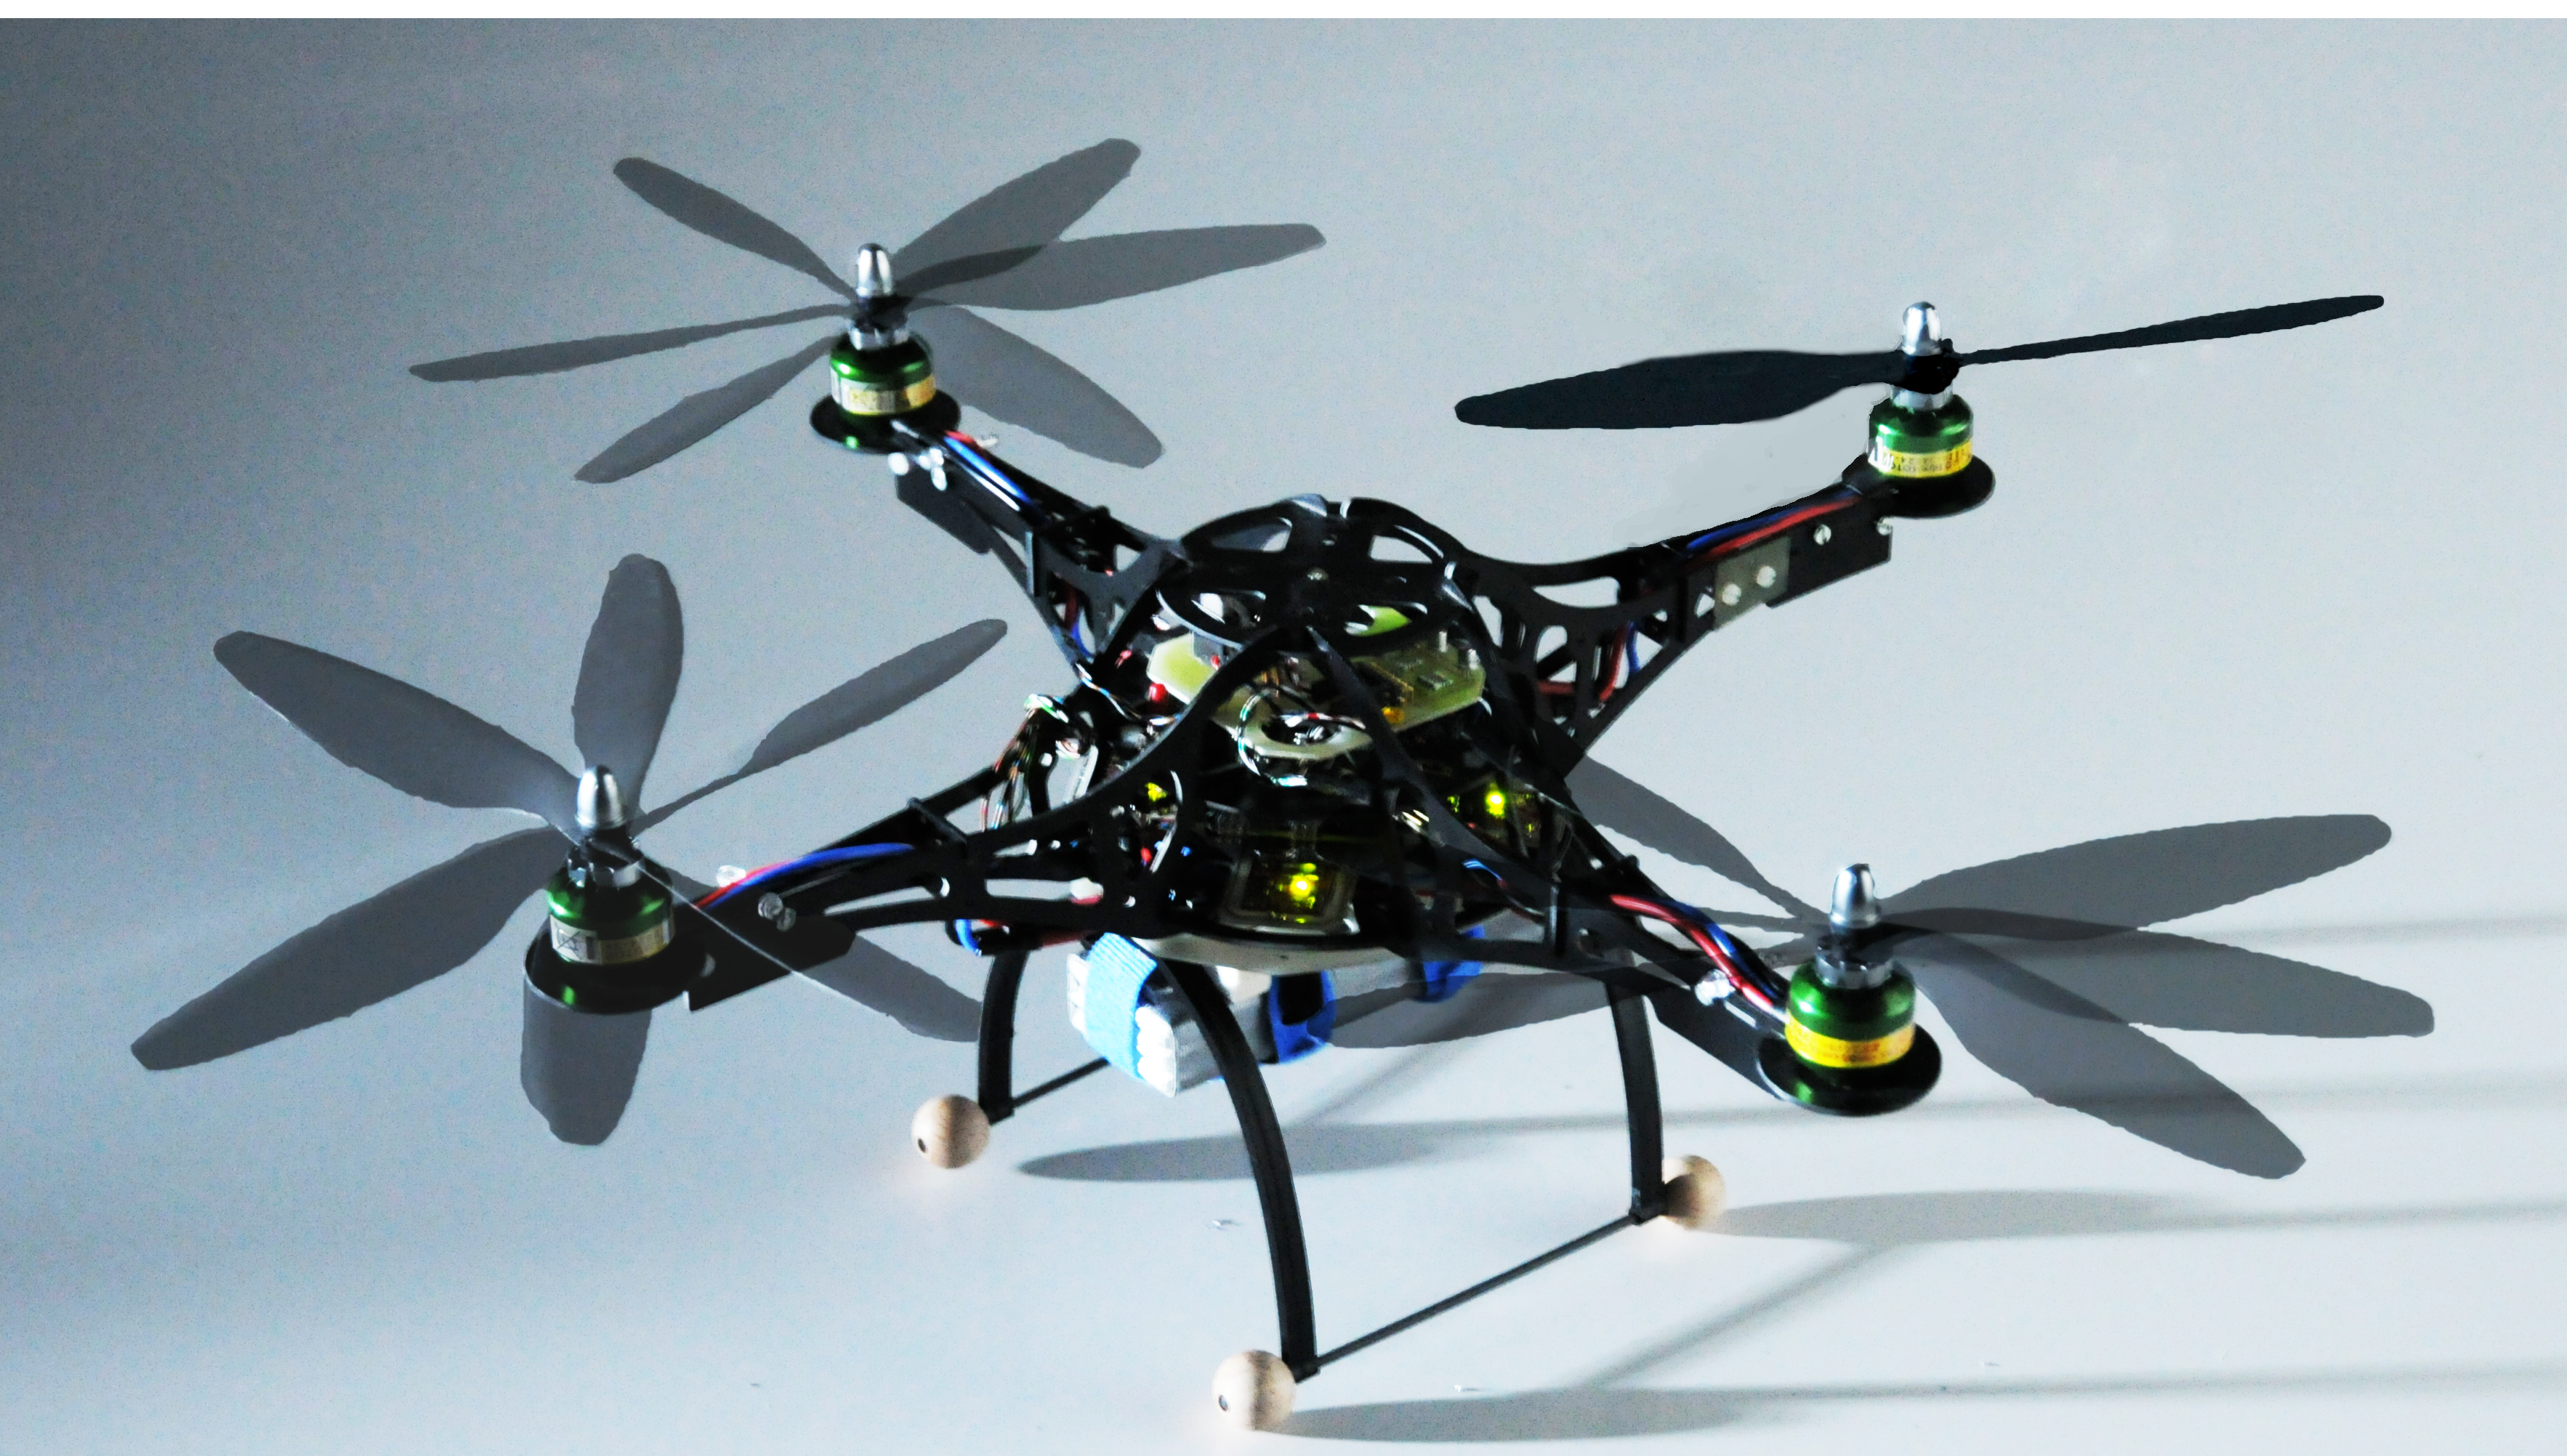
\includegraphics[width=1\textwidth]{graphic/StroboscopeRotorSpeeds.png}
	\caption{Experimental environment for set-point drift measurements}
	\label{fig:StroboscopeRotorSpeeds.png}
\end{figure}

With the execution of the described experiment, it is possible to identify the set-point drift of the particular engines. The results of the 
different set-point drift are visualised in the figure \ref{fig:Engine_Analysis.png}. The mentioned set-point of the engines is a 8bit value, which is written to the control register of the brushless controller. 
\newpage
Thereby the force, that is required to lift up the dead weight of the quadrocopter, is equivalent to the force needed for the hovering state. This force is nearby reached with the set-point of 100 on a scale from 0 to 255. As visualized in the curves in \ref{fig:Engine_Analysis.png}, the particular engines have a characteristic realization of the required set-point input, which can vary from ideal set-point.

These engine characteristics also depend to the mounted rotors and further environmental and physical behaviour which can varies over time. So the exact reconstruction of the engines' characteristics, can be unsuitable for a simulation. A better approach is to define an area different set-point drift are visualised in the figure \ref{fig:Engine_Analysis.png}.

\begin{figure}[H]
	\centering
		\includegraphics[width=1\textwidth]{graphic/Engine_Analysis.png}
	\caption{Set-point analysis of engines}
	\label{fig:Engine_Analysis.png}
\end{figure} 
\newpage
\subsection{Embedded Software Architecture}

Aspects like exchangeability, modular simulation, modular testing and dependency minimisation lead to an encapsulated modular layer design of the embedded software of the quadrocopter. The composition of the quadrocopters' embedded software, shown in the component diagram in \ref{fig:EmdeddedSoftwareArchitecture.png} \footnote{This diagram is derived from the architecture presented in \citeref[p.77 Embedded Software]{SchSunVetWebFriSat10}}, is extended with the real-time behaviour of the call hierarchy. 

Thereby modules, which use an asynchronous interrupt and a corresponding service routine to handle events are marked with a flash icon. Another important information is presented with a special dependency which contains the \gls{CT} of the component call. This value helps to understand and to research the sample behaviour of the sensors and further the control behaviour. Generally as well as in this project here, the \gls{HAL} encapsulates the control registers, which are directly related to the peripherals and the \gls{MC}, and allows a generic access to the functionality of the hardware. 

The quadrocopter \gls{HAL} contains generally five points of service access. These interfaces provide beside the service of initialisation and update of the quadrocopters' real-time image, an access to the communication with the base-station, an on board diagnosis system for noticeable visual and acoustic warnings and the access to the system timer to facilitate \gls{TT} execution in the main routine.
\newpage
Further the real-time image, located in the data layer, provides a protected access to the actual state and data of the quadrocopter. So the state of the quadrocopter is accessed by the application layer uncoupled from the \gls{HAL} and at a central data pool which allow only one state of each value. At the top level of the layer architecture, the application layer contain the control, filter and base-station communication logic of the system. Thereby the main routine uses a \gls{TT} call strategy to realise \gls{DMS} with specific \gls{CT} of the components. 

Two important points of this scheduling architecture, also described by Audsley et. al \citebib{AudBurRicWel01}, are the fact that the sum of the execution times of every routine (including \gls{ISR}) has to be smaller as the smallest deadline, which is in this case 5ms, and further the biggest deadline has to be smaller as the repeating period of execution. This constraints limit the calculation complexity of filter, control or further on-Board algorithms drastically and have to be considered in further developments and simulations.

\begin{figure}[H]
	\centering
		\includegraphics[width=1\textwidth, height=1\textwidth]{graphic/EmdeddedSoftwareArchitecture.png}
	\caption{Software components and their relationship of the Embedded System Quadrocopter}
	\label{fig:EmdeddedSoftwareArchitecture.png}
\end{figure}


\section{Adopted Approach}
\label{mt:c:DesignAndImplemetation:Adopted_approach}
After the introduction of the existing quadrocopter architecture and the analysis about the relevant characteristics of the soft- and hardware-modules, the adopted approach which will researched here is presented in this chapter. 
\newpage
Based on the introduction of the distribution approaches, presented in chapter \ref{mt:c:LiteratureReview:Distribution and implementation approaches}, the \gls{ONCA} in combination with \gls{OFIP} and \gls{SWBIP} approach will be researched here. As mentioned in the comparison of these approaches, the advantages and disadvantages are related to the aspects of interesting. So the aspects of simulation prototyping and behaviour investigation of the image processing, as well as the delay tolerances in relation to the control behaviour lead to the mentioned approach decision. As shown in figure 
\ref{fig:AdoptedApproachArchitecture.png} the adopted architecture is composed of the simulation of the base station with the corresponding image processing and the simulation of the quadrocopter components which are in focus of interest. Beginning with the set values of the embedded system, the remote control component provides time variant signals of the angular set values for roll and pitch, the angular velocity value of yaw \gls{WRT} the B-frame and the thrust value. These set values are the primary input for the body related control, which interfaces the physical model simulation with the same input values, which are provided from the \gls{CCU} and the output values. Withal the input values are transformed to a desired form, which is used for \gls{PID} control. Beside the \gls{IMU} values of the \gls{CCU}, the physical model provides an image sequence related to the position values of the quadrocopter \gls{WRT} the B-frame. Thereby the image capturing process is simulated with a high resolution underground image and the projection of the desired image resolution on it. These image sequence is provided to the simulated on-board vision system according to the \gls{ONCA} architecture. Further the vision system includes a  send process with an output image-buffer to provide the images to the base-station, and an receive process with an input correction-value-buffer.
At the other side of this wireless correspondence the base-stations' process also uses a buffered \gls{I_O}, and determines the translation (u and v) and rotational values (\gls{sym_r_of}) from the calculated \gls{OF} field.
\newpage
Finally the additional controller, which realises the drift elimination in the hovering state, is located in the quadrocopter system and observes the set values of the remote control. The idea thereby is to find a value state of the set and sensor values, which symbolises that the hovering state is desired by the pilot and further the quadrocopter body is ready to reach that state. To realise that behaviour a state machine, which is located in the module "Check Hovering State", decides in real-time the activation of the visual system. So the set values of a second controller, that is located in the separate position control module, are switched from zero to the received correction values. This has the effect that the body controller is delegated by the second position controller and corrects the position with a correction flight manoeuvre. If the pilot sends new set values, after the quadrocopter has reached the hovering state, the position controller is deactivated and allows the pilot and further the body controller an uninterrupted flight and batch-processing of set values. 
% Why state machine observes just set values?
% Description of Distributed error correction scheme

\begin{figure}[H]
	\centering
		\includegraphics[width=1\textwidth]{graphic/AdoptedApproachArchitecture.png}
	\caption{Adopted approaches' architecture}
	\label{fig:AdoptedApproachArchitecture.png}
\end{figure}

%\subsection{Optical Flow Approach}
%Short overview of approaches Ref to chapter 3.2.4. Why block matching -> fundamental approach, less parameters to configure.
%Describe the Optical Flow interpretation
%Generally two of the classifications of \gls{OF} algorithms are given with algorithms which uses a feature tracker and algorithms which search pixel groups, called blocks, between the sequence of images. The feature tracker algorithms first determine good trackable features. This features used as base, and searched in the following sequence of images. The vectors, calculated between these sequence of features, result the \gls{OF} field. In this project here, this kind of \gls{OF} determination is used with a corner detection process as feature tracker. In the other hand, a block matching algorithm is used to fulfil a comparison of two algorithms of different classifications. Beside the specific algorithm of the \gls{OF} determination, the calculation and processing of the vector field also represents an important topic of investigation. The approaches used here are visualised ...

\subsection{Control Approach}
\label{mt:c:DesignAndImplemetation:Adopted_approach:Control_Approach}
Before starting the design of the quadrocopter controller, it is helpful to understand and analyse the abstract behaviour of the separated, physical processes and to proof the correct function of the approach. This strategy lead in this project here to the construction of a simulation which shows the behaviour of realising an angular set-point value to one axis of the quadrocopter, which include two engines as actuators. As visualised in figure \ref{fig:QuadrocopterPhysicalModel}, two opposing engines realise the angle movements in the specific pitch- or roll-axis. These engines can realise an individual gain to the given set-point and influence the precision of the control system. Another point which is problematically in this case is the fact that the feedback angle acceleration of the \gls{CLCS}, has to be integrated two times. 

The combination of the unprecise gain of the engines and the two integrations influences the stability of the \gls{CLCS} enormous. To simulate this behaviour and to impart the expected effects, a abstract simulation is build up and executed in Simulink with two configurations. As visualised in \ref{fig:PIDCascadeCtrl.png} the plant includes two engines, simulated as a sequence of a direction and individual gain. Furthermore two integrators transform the angular acceleration to a angular velocity and position which is used for feedback for the cascaded \gls{PID}-Controllers. This feedback is designed as switch which can be interrupted, to fulfil a tests scenarios with single and cascaded 
\gls{PID} control approaches.

\begin{figure}[H]
	\centering
		\includegraphics[width=1\textwidth]{graphic/PIDCascadeCtrl.png}
	\caption{Abstract CLCS of one angle}
	\label{fig:PIDCascadeCtrl.png}
\end{figure}

As introduced in chapter \ref{mt:c:literature:s:Control_Systems_Characteristics}, the stability behaviour of \gls{CLCS} can be shown with a pole diagram and the investigation of the location of the poles (See Pole Map \ref{fig:PIDCascadeDiagrams.png}). Another method, to proof the stability in the frequency domain, is given with the Nyquist Criterion \citeref[pp. 487-493, Relative stability and Nyquist Criterion]{DorBis01} and describes that each integration in a system affect a shift of \ensuremath{90�} of the frequency phase. The criterion describes that the phase at the x-axis' point of 0dB of the corresponding gain has to be bigger as \ensuremath{-180�}. So also this theorem proofs, that the determination of a value which passes two integrators, must have a \gls{PID}-cascade to ensure that the feedback prevents a critical frequency phase shift.

These relations are visualised as bode diagram in figure \ref{fig:PIDCascadeDiagrams.png} with logarithmic axis of the gain, frequency and phase. Furthermore the step response of the \gls{PID}-cascade and the single feedback \gls{PID}-controller (See Step Response \ref{fig:PIDCascadeDiagrams.png}) shows the stable and the oscillating unstable behaviour of these configurations.

 
\begin{figure}[H]
\subfigure{\includegraphics[width=0.33\textwidth]{graphic/PIDCascadeDiagrams_1.png}}%\hfill
\subfigure{\includegraphics[width=0.33\textwidth]{graphic/PIDCascadeDiagrams_2.png}}
\subfigure{\includegraphics[width=0.33\textwidth]{graphic/PIDCascadeDiagrams_3.png}}
	\caption{Pole Diagram, Bode Diagram and Step Response of one angle system}
	\label{fig:PIDCascadeDiagrams.png}
\end{figure}


\subsection{Problems, Limitations and Assumptions}
\label{mt:c:DesignAndImplemetation:Problems_Limitations_and_Assumptions}
This chapter focus the existing problems in the real implementation of a distributed, visual drift correction scheme
of \gls{UAV}, and shows abstractions and assumptions that are made for the structure and implementation of this projects' simulation.
Such characteristics can be separated into domains, which provide the basis of problem and limitation analysis and allow to define a
abstraction level. This abstraction level can be used to focus and analyse, just the characteristics of a specific part of a solution. This allows to concretise and locate problematic behaviour before searching for a solution at a wrong section. A concrete example for this argumentation can be given by regarding the camera domain. 

Characteristics like the focal length influences the sharpness of the image and influences the 
image processing algorithm to calculate the \gls{OF}. But this characteristic can be classified as problem, that has to be solved after the characteristics of more basic problems has been investigated. 
\newpage
The focal length f can be abstracted with setting the height Z, between the image plane of an ideal projection model and the underground, equal to f and to assign both values the fixed value of one meter. This allows to project the values of the ground points \ensuremath{P=(X, Y, 1)^{T}} directly to points on the image plane \ensuremath{p=(x, y, 1)^{T}} 
\footnote{A detailed mathematical deviation of this abstraction presented in \citeref[Chapter 2, pp.15-16 instructions of transformation]{Fac08}}. Further assumptions of the camera domain are, the camera does not create distortions 
\footnote{This fact also is implicated with the usage of the ideal projection model}, the optical axis is projected rectangular to the underground \footnote{This implicates that the camera movement is planar to the ground and the camera is mounted correctly on the \gls{UAV}. This assumption is adopted from \citeref[p.78 Motion Model Deduction]{Wei09}} and the exposure of the environment is constant over time
\footnote{Experiments with a real camera involve a correct camera calibration (see appendix 
\ref{mt:c:Appendix:Mathematical_description_of_distortions}), and a environment preparation of the exposure to realise these characteristics}.
So the assumption in relation of the \gls{DOF} of the camera system can be described as same as the \gls{DOF} of the quadrocopter body, but reduced in the rotational movements around the axis which originates in the middle of the image plane. The quadrocopter body domain defines the behaviour of the movements of the hovering state, which can be assumed as a 5 \gls{DOF} by reducing the movements across the axis \ensuremath{Z_B}. The realization of these two different \gls{DOF} system can be realized with a real-time image correction process as described in 
\ref{mt:c:Appendix:Mathematical_description_of_distortions} or with a hinge mechanism which keeps the image plane planar to the ground. 

In the simulation this assumed state of the camera domain is realised with a state machine and the orthogonal projection of a simulated camera image on a underground image, as mentioned in chapter \ref{mt:c:DesignAndImplemetation:Adopted_approach}. Another domain, which includes limitations and has to be defined here, is given with the underground domain. The related assumptions to this domain, are that no objects exist, which moving relative to the quadrocopter e.g. no moving light reflections, and the underground image contains points and contrast,
\newpage
which can be evaluated in the \gls{OF} algorithm. For example, an underground image of a snow-covered landscape which contains segments with no contrast is not usable for this approach. Finally the communication between the base-station and the quadrocopter is abstracted as delay. This abstraction excludes communication fail, synchronisation or segmentation problems and assumes a smooth operation of the image and correction value transmission and reception. This behaviour is also symbolised with synchronous buffering systems in figure \ref{fig:AdoptedApproachArchitecture.png}.

\begin{figure}[H]
	\centering
		\includegraphics[width=1\textwidth]{graphic/ProblemAndLimitationDomains.png}
	\caption{Problems and limitations separated in domains}
	\label{fig:ProblemAndLimitationDomains.png}
\end{figure}

% Description of abstractions and assumptions
% Starting Problem of image processing
% Angle of the camera
% Distortions
% Light effects
% Noise
% Problem of relative moving Objects -> Background estimation
% Problem of captured underground -> Snow no features? etc.
% Directory Problem of yaw causes sign of vector
% Aperture Problem

%Assumption 1 Vehicle moves on a planar ground plane. This assumption is true
%for vehicle under most circumstances and it limits the degrees of freedom of the vehicle
%moving on this plane. [Wei09, S.74]
% How I guarantee this in the implementation? -> State Machine
%
%Assumption 3 The XZ plane of the camera frame is parallel to the ground plane.
%This assumption is valid if the camera is mounted on the vehicle correctly.  [Wei09, S.78]
% How How can I simulate such thing? -> Image Projection on large image 

%Assumption 4. Communication is abstracted as delay, no errors no copies no synchronisation
%problems, etc.
%Der Kommentierte Text wurde in diesem Kapitel eingebaut

\section{Simulation of Embedded System Quadrocopter}
\label{mt:c:design:Simulation of Embedded System Quadrocopter}
The architecture of the embedded system simulation is constructed by following the modular design.
\newpage
The focus of this execution was to full-fill the aim of an exchangeable and flexible simulation architecture, which can be changed and reconfigured with minimal effort. This design criteria results to the architecture of Simulink modules as visualised in \ref{fig:SimEmbSysQuadro.png}, and allows a hierarchical realisation of the quadrocopters' system simulation. The separation of modules contains a control library which allows to use several control modules in relation to the development state.
As shown, the first development is executed as prototype in a native Simulink model without having complexity or resource limitations. This model is refined to an embedded \gls{MATLAB} model, which contains only Matlab code which is cyclic executed. This refinement allows to simulate the quantisation and limitation behaviour of an embedded controller and further to evaluate if the implementation algorithm works correctly. The last step is to implement or to generate the embedded controller to the quadrocopters' embedded system target language C, and to evaluate this with the \gls{HIL} module over a serial interface. This last step includes aspects like resource limitation analysis, algorithmic calculation complexity etc. 

Based on this method, this project here focus the development of a Simulink controller in the abstract level by using the \gls{IMU} and \gls{OC}, which can be implemented and realised in the same way as the existing control algorithm which controls only by using the \gls{IMU}. The sensors and actuators are grouped in a own library and allow generic customisation of a sensor and actuator model and can be exchanged if the real hardware is changed. This exchange behaviour is also given in other components of the embedded quadrocopter system simulation and can be extended with implementation of new modules \gls{WRT} the interface architecture.
\newpage
The optical-sensor has a special function in this project. It allows running tests and simulations of the quadrocopter system with a reduced simulation complexity. This is fulfilled because this module can generate the behaviour of the image processing signal with mathematical functions and can so reduce the simulations' execution time. Finally the utility library contains tools for analysis, visualisation and steering of the quadrocopter simulation, which have an important function in the performance test process of this project.  

\begin{figure}[H]
	\centering
		\includegraphics[width=1\textwidth, height=1\textwidth]{graphic/SimEmbSysQuadro.png}
	\caption{Modular overview of the Embedded Quadrocopter System Simulation}
	\label{fig:SimEmbSysQuadro.png}
\end{figure}

The customised embedded quadrocopter system architecture is shown in figure \ref{fig:CustomEmbSysQuadro.png} as Simulink model, which contains a \gls{CLCS} architecture. The set-values from the remote control can be generated in different ways and support a virtual flight with a 3D-mouse or further a flight manoeuvre constellation of steering values. This signal is a composition of pulses defined with the Heaviside-function \footnote{See \citebib{Wei11}} and multiplied with ramp-signals and can be accessed for batch-simulation. 

These set values are realized in motor values by the control component. This component executes, with respect to the mentioned development state, a controller simulation till a \gls{HIL} communication. In each case the controller knowledge of the quadrocopter movements are provided by the sensors. In this special customisation the input signals of the sensors are provided by the Dynamics block and can be assumed as optimal. 

Thereby the sensor block provides the signal with disturbances like noise and quantisation as in reality. Further the correction values for the drift elimination are already known by the  sensor block and can be also disturbed by regarding the signal quality of the optical movement detection. Another way to determine these correction values is to send these via the output of this model to the base station and to receive the corresponding correction.

The signal pos-vel-acc includes all signals, produced by the Dynamics block, and provides a generic interface between the related collaborative blocks. Another strategy to test the stability of the control algorithm is the generation of environmental influences. This can be executed  similar to the remote control with the generation of a velocity vector signal stimuli, which is add as error to the actual optimal velocity value calculated by the \gls{EOM}. 
\newpage
To provide the opportunity of batch-processing-simulation, the error signals can also be accessed outside the model. 


\begin{figure}[H]
	\centering
		\includegraphics[width=1\textwidth]{graphic/CustomEmbSysQuadro.png}
	\caption{The customised CLCS architecture in Simulink}
	\label{fig:CustomEmbSysQuadro.png}
\end{figure}

\subsection{Flight Dynamics}
% Realizations of Flight Dynamics -> Inputs and Outputs errors
% Results from the Thrust to Seitpoint Curves in chapter 4.1.2
%% Further characteristics of motors
% Input transformation process output?
\label{mt:c:DesignAndImplemetation:Flight_dynamics}
The realisation of the dynamics block in Simulink is based on the researches presented in chapter 
\ref{mt:c:design:Analysis of Existing Quadrocopter Architecture:Characteristics of Sensors and Actuators} and on the 
\gls{EOM} presented in chapter 
\ref{mt:c:literature:s:equations_of_motion}. First the derived \gls{GAV} \gls{sym_dot_zeta} \gls{WRT} the H-frame was analysed to determine the dependencies of the \gls{ODE}. Based on that, the physical model was build up  with the aim to ascertain all positions, velocities and accelerations of the quadrocopter body, that is required for this project. The result is presented in a schematic view in the figure 
\ref{fig:SimulinkImplementationOfDynamics.png}. Thereby this module gets the register set-values, corresponding to the brushless controllers in the reality (See\ref{mt:c:design:Analysis of Existing Quadrocopter Architecture:Characteristics of Sensors and Actuators}), and passes the mentioned pos-vel-acc vector to the next block.
\newpage 
In this process the actuators engine blocks transform the set-point to a corresponding force \ensuremath{F_n} \footnote{The index n stands for the number of engine and ranges from 1 to 4} and \gls{RPM} value \ensuremath{\Omega_n} (See \ref{mt:c:DesignAndImplemetation:Sensors_and_Actuators}). 

These values of the different motors are composed to the movements \ensuremath{U_n}, by executing the calculations presented in equation \ref{formula:EB_Omega2} and further to the resulting \gls{RPM} value \ensuremath{\Omega}. Furthermore, these output values are passed to the calculations, which based on the component \gls{sym_dot_omega_B} \gls{WRT} the B-frame of the equation \ref{formula:dot_zeta}. To determine the velocity and the angle, this vector is integrated two times. A special behaviour of this block is that the calculation of the \gls{sym_dot_omega_B} needs also its own values. So the start values have to be initialised in this case for the initial execution with the values zero. Equivalent to the B-frame component of \gls{sym_dot_zeta}, the E-frame component \gls{sym_ddot_Gamma_E} from the equation \ref{formula:dot_zeta} is used to calculate the translation acceleration, velocity and position vectors. Thereby the translations also passed trough two integration processes. 

\begin{figure}[H]
	\centering
		\includegraphics[width=1\textwidth]{graphic/SimulinkImplementationOfDynamics.png}
	\caption{Schematic realisation of Dynamics Module }
	\label{fig:SimulinkImplementationOfDynamics.png}
\end{figure}

These calculated values are combined to the output vector and provided as output. The \gls{GVV} \gls{sym_V_B}, which is needed to simulate the on-board behaviour of the acceleration sensor, is determined with the inverse rotational matrix multiplied with translation \gls{GVV} \gls{sym_Gamma_E}. The generic aspect of this approach is that a generally \gls{EOM} dynamics model also will have the same output values and will be compatible to the same interface, if it has 6 or less \gls{DOF}. Furthermore the determination of all movement values allows the simulation of future developments with each kind of movement detection sensor.

\subsection{Control}
% Realization of control approach -> Inputs, Outputs Design Cascade
Observing the analysed control behaviour, presented in chapter \ref{mt:c:DesignAndImplemetation:Adopted_approach:Control_Approach}, the final quadrocopter controller is a \gls{MIMO} controller, which includes several cascaded \gls{PID} \gls{SISO} controllers. The figure 
\ref{fig:QuadrocopterControlArchitecture.png} visualises the detailed controller architecture. Starting at the input values of the control module the angular velocities, the translational acceleration values and the set values are combined for control usage. Thereby the different sources of the values are symbolised with superscript symbols like "Gyr" for gyroscope, "Opt" for optical sensor, "Acc" for acceleration sensor and "Set" for set-value. These input values run first through a process of transformation, which converts the raw sensor values to usable physical values for the control process. In this case the angles for pitch and roll are not determined with an integration but are calculated using the translational accelerations of the corresponding rotation axis. 
\newpage
This is possible because the gravitational orthogonal force is related to these rotations and can be used to determine the angles without an integration process. The conversion of raw- to physical-values, presented in chapter \ref{mt:c:design:Analysis_of_Existing_Quadrocopter_Architecture:Central_Control_Unit}, allows an easier control realisation and processing. 

\begin{figure}[H]
	\centering
		\includegraphics[width=1\textwidth]{graphic/QuadrocopterControlArchitecture.png}
	\caption{Quadrocopter Control Architecture}
	\label{fig:QuadrocopterControlArchitecture.png}
\end{figure}

The converted physical values are passed to the position-correction and body-control-process. Thereby the position-correction-process passes the set-values to an internal state-machine which detects the hovering state and activates the position-correction-controllers. For realising this, the state-machine checks the set-values of the angles and checks if these are smaller as a defined threshold, which symbolises that there is no activity of the remote control. After reaching this threshold the state-machine switches to a state which delays the activation of the position-correction-controller for the duration of \ensuremath{t_{wait}}. 
\newpage
This delay is needed for the body controller and the related cascaded \gls{PID} controllers to reach the steady-state of the hovering position. The activation of the position-controllers, which try to minimise the input values of the optical sensor, affects that the output values of these controllers are integrated to the first stage of the cascaded \gls{PID} controller in the body control. The result is that this collaboration of the controllers affect the needed behaviour for position correction of the hovering state, because the error value of one controller architecture is passed as set-value to the other architecture. Finally the cascaded \gls{PID} control realises movements given from remote control, or manoeuvres needed for position correction, and passes the angular values to a conversion block for the motor set-points. This block realises the variations of the particular motors by realising the desired thrust set-value \ensuremath{U_1}. Another important characteristic in the design of this simulation is the option to run the body and position-control \gls{PID} controllers with different sample times (\ensuremath{t_{s}^{opt}} and \ensuremath{t_{s}^{imu}}). This behaviour originates form the facts, that the \gls{IMU} sensors can provide a higher sample rate as the optical sensor, and the sample rate can influence the characteristics of a \gls{CLCS} (See \ref{mt:c:literature:s:Stability_criteria_of_transfer_functions}).



\subsection{Sensors and Actuators}
\label{mt:c:DesignAndImplemetation:Sensors_and_Actuators}
A simulated dynamic model, as introduced in chapter \ref{mt:c:DesignAndImplemetation:Flight_dynamics}, provides as mentioned optimal movement  signals, which does not reflect the reality. So an artificial process which creates a disturbing signal fused with the optimal signal, can be used to investigate and simulate the realistic behaviour of the sensors and actuators. These characteristics are also regarded in this project here with the result to transform the optimal signals with the experienced knowledge of chapter \ref{mt:c:design:Analysis of Existing Quadrocopter Architecture:Characteristics of Sensors and Actuators}.
\newpage
The results are presented as Simulink models in \ref{fig:SensorsAndActuators.png}. 
Both components, sensor and actuator, contain similar functions to limit and amplify (Saturation and Gain) the incoming signal. Gyroscope and acceleration-Sensors further contain a quantification, offset and noise process to fulfil these typical effects. The sensor model can so be customised individually by configuring these mentioned characteristics, and provides a model close to reality. In the other hand, the actuator model provides only one configurable characteristic, the motor gain, which is used to simulate the error characteristic of the engines presented in chapter 
\ref{mt:c:design:Analysis of Existing Quadrocopter Architecture:Characteristics of Sensors and Actuators}. Beside this the brushless motors access the same, experimental determined tables for the set-point to thrust and thrust to \gls{RPM} conversion.
 Important thereby is that these conversion tables realise a non-linear relation between the set-point and thrust, like in the reality.
 Further the important behaviour of the actuator delay is simulated as a delay process in the frequency domain.
The presented generic blocks in this chapter, are customised once for the simulation of the existing hardware of the quadrocopter and integrated in the sensor module \gls{CLCS} shown in figure \ref{fig:CustomEmbSysQuadro.png}. So in focus of this project here, the characteristics of these blocks are not varied for further investigations.    

\begin{figure}[H]
	\centering
		\includegraphics[width=1\textwidth]{graphic/SensorsAndActuators.png}
	\caption{Sensors and Actuators}
	\label{fig:SensorsAndActuators.png}
\end{figure}

\section{Simulation of Base Station}
The aims considered in the base stations' simulation are the exchangeability of image processing algorithms and modules and further the ability to vary characteristics of the captured images. The aspect of algorithm exchangeability is realised with an architecture, which separates the image processing from interpretation of the derived values. Regarding this aspect, different image processing modules provide different form of values. As shown in figure \ref{fig:SimBaseStation.png} the \gls{OF} algorithms are also logically separated in high and low level algorithms. This hierarchy architecture aspect provides the ability to mix high and low level algorithms from different frameworks. 

Beside the algorithm architecture, the simulation of the base station provides several variations of source and sink of the processed video. The source thereby can be an synthetic video, which is generated with the assumptions mentioned in chapter 
\ref{mt:c:DesignAndImplemetation:Problems_Limitations_and_Assumptions}, or a real captured video. Thereby the synthetic video provides the ability to vary the image size and frame rate, which can not be executed in real videos. Similar to the simulation of the embedded system quadrocopter, the movements of the camera view can be steered with the remote control module or with the environmental influences.

Thereby the environmental influences can provide a desired trajectory with variable velocity or acceleration, which can be used as reference to evaluate the quality of optical movement detection. Finally the analysis lab, as mentioned in the embedded system quadrocopter simulation, also provides the option to observe and analyse customised models, build up with the modules of this simulation. 

\begin{figure}[H]
	\centering
		\includegraphics[width=1\textwidth]{graphic/SimBaseStation.png}
	\caption{Simulation of Base Station}
	\label{fig:SimBaseStation.png}
\end{figure}

\subsection{Video Sources: Synthetic Video vs. Real Video}
%Abstraction of Video model, Abstraction of angle -> Potential solution for that derived from Ter10
As mentioned, the video input of the optical movement detection process can be created synthetic, or a real captured video can be used. Regarding the synthetic video, the frame rate and image size can be configured because the generation of the image stream is created with a transformation of the image window executed on the ground image. 
\newpage
This transformation is executed using a transformation matrix, which describes the translation and rotation of the next image. The sample-rate configuration thereby is realised in the integral, which contains the sample time \ensuremath{t_{s}^{Opt}} of the image capture. In contrast to that, the real video source process, can just decrease the sample rate by selecting and forwarding each \ensuremath{n^{th}} image. Further it is not possible to determine the trajectory of the image movement, because the video caption was executed with the relation to the physical movement of the camera \footnote{The synthetic video architecture is derived from video mosaicking memo, presented at http://www.mathworks.com/help/toolbox/vision/}.

It can be summarised that the synthetic video can be used for prototyping and executing test cases. The benefit thereby is that the possibility to capture measures, influenced by unexpected effects, is very low and the input-data of the test cases is created and realised exactly. So the experimental results can be regarded as isolated from unexpected influences and can provide the essential behaviour of the tested components. 
In the other hand the real video provides a realistic trajectory scenario, which contains a lot of influences like distortions, light effects, noise and so far. So the real video approach can help to fine tune filters and to optimise the image processing, but should not be used for the initial prototyping steps of development. Another important aspect in the real video approach is that the trajectory should be measured in real world, with a reliable measurement configuration. This has to be a great deal more precise as the expected precision of the image processing, to prevent misjudgements of the evaluated results.

All in one, the synthetic video approach is suitable for the first prototyping simulations and the real video for the final fine tuning. The challenge thereby is the crossing level from synthetic to real video. 
\newpage
That means the synthetic video simulation has to reach as much as possible the real video, before the exchange of the video sources can be executed.


\begin{figure}[H]
	\centering
		\includegraphics[width=1\textwidth]{graphic/SyntheticVsRealVideo.png}
	\caption{Synthetic Video generation and Real Video}
	\label{fig:SyntheticVsRealVideo.png}
\end{figure}
 
\subsection{Calculations}
The interpretation of the optical flow is executed in two different ways in this project here. These approaches, mentioned in the architecture overview \ref{fig:SimBaseStation.png} as calculations, provide the same output with different input representations. 
\newpage
The first approach, presented by Termtanasombat \citebib{Ter10}, is called \gls{FNC}\footnote{This approach is presented in figure \ref{fig:SimBaseStation.png} as Vectors Movement Calc.} and determines the quantity of the optical flow by calculating the average of optical flow over the magnitude of the velocity vectors. A similar calculation is visualised in figure 
\ref{fig:RawAndAverageOF.png}, with the difference that the velocity vectors of the raw optical flow are represented as complex numbers. Further the average calculation is executed with the accumulation of the average of the imaginary and real part in each direction. This resulting vectors are symbolised with \ensuremath{\omega_{i}} with the index corresponding to the direction and axis. Thereby, the assumptions presented in chapter 
\ref{mt:c:DesignAndImplemetation:Problems_Limitations_and_Assumptions} allow the mentioned movement set, which does not contain the movements in \ensuremath{Z_B} direction and a corresponding \gls{FOE} \footnote{Such a \gls{FOE} is shown e.g. in the middle of the raw optical flow in figure \ref{fig:RawAndAverageOF.png}}.

\begin{figure}[H]
	\centering
		\includegraphics[width=1\textwidth]{graphic/RawAndAverageOF.png}
	\caption{Averaging process of Raw Optical Flow Field}
	\label{fig:RawAndAverageOF.png}
\end{figure}

The defined \gls{DOF} allow to calculate the desired velocity values of movement from the average optical flow. This procedure is shown in figure \ref{fig:RotTransFromOF.png}. There we can see a combination of rotational and translational movement as average optical flow. First, to determine the rotational movement, the smallest magnitude of the velocity vectors is the used as indicator. 
\newpage
The idea behind that is, that the rotation around the centre of the image is represented in each average velocity vector. Additionally, just a rotational movement can influence in parallel all four average velocity vectors. So the separation of the translational and rotational movements can be executed with subtract the constant rotational offset, represented in the circle, from each average velocity vector. The complement results a translational combination of the vectors in \ensuremath{X_B} and \ensuremath{Y_B} direction. A problem of this described interpretation of the rotational component is the missing information of the rotation direction. Consequently the direction of rotation has to be adopted from the yaw gyroscope sensor. 

\begin{figure}[H]
	\centering
		\includegraphics[width=1\textwidth]{graphic/RotTransFromOF.png}
	\caption{Determination of rotational and translational component with the Flow Number Calculation approach}
	\label{fig:RotTransFromOF.png}
\end{figure}

Another approach to determine the desired translation and rotation velocities is to determine the \gls{Tform}\footnote{This approach is presented in figure \ref{fig:SimBaseStation.png} as T-Matrix Movement Calc.} between two images in an image sequence. In this project here, the tracked features of both images are represented as two dimensional points. An algorithm, which estimates the movement of the points 
, called \gls{RANSAC}, provides the determination of the \gls{Tform} in each sample step.
\newpage
Furthermore, this matrix contain information of rotation and translation which allows the determination of these values with a reverse calculation shown in figure \ref{fig:RotTransFromCOOF.png}. Combined with the known sample time of the image sequence, the determined angle and translation positions can be transformed to velocities. The important characteristic of the \gls{Tform} calculation is given with the determinable direction of the rotation movement.

\begin{figure}[H]
	\centering
		\includegraphics[width=1\textwidth]{graphic/RotTransFromCOOF.png}
	\caption{Determination of rotational and translational component with the Transformation Matrix approach}
	\label{fig:RotTransFromCOOF.png}
\end{figure}

\section{Optical Movement Detection Architectures}
\label{mt:c:design:Optical Movement Detection Architectures}
The presented optical movement detection algorithms and calculations can be realised in several ways of implementation. Two of these approaches are introduced and described in this chapter. One approach is given with the Video-and-Image-Processing-toolkit~\copyright~of MATLAB/Simulink. 
This toolkit provides an easy and fast way to realise image and video algorithms, using the \gls{MBD} approach. This way of development brings a lot of advantages, but also disadvantages. 
\newpage
Another possibility to realise image and video processing algorithms is given with OpenCV (See chapter \ref{mt:c:pm:openCV}). This framework allows, as mentioned, the usage of a huge amount of optical algorithms and provides further very detailed configurations of these. But why it is not possible to use just one of these two optical movement detection architectures? The problem is that each of these architectures has strengths and weaknesses. In the development of the base stations' image processing, the realisation was executed in MATLAB/Simulink. Regarding the necessity of spiral model to present with less effort a first running prototype, the MATLAB/Simulink-Native \gls{VIP} is better suited. As presented in chapter \ref{mt:c:pm:Strengths and Risks} the limited amount of algorithms of the \gls{MBD} framework can become a drawback for extensions and refinements of the realised \gls{VIP} architecture. So it is important to have the ability to extend manually the \gls{VIP} algorithms of the \gls{MBD} tool. Such extension can be executed with MATLAB/Simulinks' Mex-Architecture (See chapter \ref{mt:c:pm:MATLABSimulink}). The following table \ref{fig:MATALBSimulinkVSOpenCV} introduces some important characteristics of both frameworks, and shows the advantages and deficits of these. 
 
\begin{figure}[H]
	\centering
		\includegraphics[width=1\textwidth]{graphic/ComparisionOpenCVSimulink.pdf}
	\caption{A comparison between MATLAB/Simulink-Native VIP and OpenCV VIP}
  \label{fig:MATALBSimulinkVSOpenCV}
\end{figure}

%\begin{table}
%\begin{tabular}{|l|p{7cm}|p{7cm}|}
%\hline
 %& MATLAB/Simulink-Native VIP & OpenCV VIP\\
%\hline
%\hline
%\multirow{3}{*}{Pros} & Support of automated target code generation & Provides exact configuration interfaces  \\
%\cline{2-3}
 %& Easy to configure and to maintain & Big amount of algorithms\\
%\cline{2-3}
 %& Easy to learn &  Easier to unify to special implementations causes C++ object oriented paradigm \\
%\hline
%\multirow{3}{*}{Cons} & Limited amount of algorithms & Flexibility of configuration and maintenance is related programmed architecture\\
%\cline{2-3}
 %& Supports not detailed configuration & Does not support MDB paradigm. Code must be written manually\\
%\cline{2-3}
 %& Limited unification of algorithms possible & Difficult to learn. Complex architecture\\
%\hline
%\end{tabular}
%\caption{\label{fig:MATALBSimulinkVSOpenCV} A comparison of MATLAB/Simulink-Native VIP and OpenCV VIP}
%\end{table}

%Describe the several options of optical flow algorithms discussion of Lucas Kanade, Horn Schunk and block matching
%Describe generic architecture of this MATLAB/Simulink program
%-> MATLAB Native
%-> OpenCV and the bridge to MATLAB
%-> others
%\subsection{Matlab Optical Flow Algorithms}
%Presentation and dicussion of Lucas Kanade, Horn Schunk and block matching in MATLAB
% Advantages of MATLAB/Simulink algorithms
% Support of automated target code generation
% Easy to configure and to maintain
% Easy to learn/understand
% Good Error handling environment with logical check of values and configurations
% Includes various interfaces of MATLAB/Simulink architecture for other libs and tools

% Disadvantages of MATLAB/Simulink algorithms
% Limited amount of algorithms
% Supports not detailed configuration
% Limited unification of algorithms possible
% Complexity of algorithms or target complexity analysis not possible
% Commercial

%Presentation and dicussion of Lucas Kanade, Horn Schunk in OpenCV and more new algorithms like Feature tracker
% Advantages of OpenCV algorithms
% Faster as MATLAB/Simulink
% More algorithms
% More exact configuration
% Easier to unify to special implementations causes C and OpenCV architecure
% Easier to identify complexity of algorithms and the runtime behaviour in real architecure causes less abstraction
% Open Source

% Disadvantages of OpenCV algorithms
% Difficult to learn and to configure
% Difficult to identify logical errors in configuration or implementation
% Problems with compatibility with other libs and tools -> workaround necessary as in EsmSna08
% No support for automated target code generation
%\subsubsection{Extensions}
%Point to further implementation and Test modules e.g. for angles blur noise etc.

%\section{Test Environment}
%Architecture of MIL
%Simulation Tests
%MIL Tests

% -----------------------------------------------------------------------------------------

% PAGES: 10
\chapter{Experimental Results and Analysis}
\label{mt:c:expResults}

The following chapters present the examined results and analysed aspects. First the image processing characteristics are analysed with test scenarios, which focus the interesting aspects of investigation. Each test scenario contains beside the description of the investigated domains, also the expected results of the experiments.
These expectations are compared, with the results of the experiments and discussed. After the analysis of the image processing, the chapter 
\ref{mt:c:expResults:AnalysisofControlbehaviour} shows the characteristics and optimisation of the control architecture and the analysis and tune strategy of the control system. Finally the analysis of the position correction scheme in chapter 
\ref{mt:c:expResults:AnalysisofPositionCorrectionScheme}, focus the complete position correction system and combines the previous analysed results together. Thereby different scenarios are executed with different configurations and disturbances. Furthermore a final analysis also demonstrate the hovering state characteristics of the focused configurations.

\section{Analysis of Image Processing}
\label{mt:c:expResults:AnalysisofImageProcessing}
This section introduces the specifically configured test environment and the corresponding results of the analysed topics, related to the motion detection. Furthermore, the testing analysis is separated in three domains of variation, presented in figure 
\ref{fig:ImageProcessingAnalysisDomains.png}. The basic idea thereby is to create a 2D-trajectory by using a stimulus as evaluation source of the results. This stimulus can be executed in three types of motion, presented in the stimuli domain. Basically, the stimulus is given as rotational or translational velocity type, which also provides an output value from the image processing. Additionally, to test the reaction behaviour of the a image processing configuration, it is important to use velocity steps, or further, acceleration inputs. Such tests show how fast the changed value can be reached by image processing, and give a measure for the time impact.
Another domain that can be separated for the tests here is the algorithm and calculation domain. As visualised, this segmentation can be structured as a tree with n nodes which contain the image processing algorithms and calculations as leaf nodes. As mentioned, in this project here the algorithm and calculation constellation is reduced to the two visualised combinations, for reasons of algorithm support of the used simulation framework.

\begin{figure}[H]
	\centering
		\includegraphics[width=1\textwidth]{graphic/ImageProcessingAnalysisDomains.png}
	\caption{Image processing analysis domains in focus of this project}
	\label{fig:ImageProcessingAnalysisDomains.png}
\end{figure}

Finally, the regarded aspects in relation to this project of the video source behaviour are summarised in the video domain. To provide a realistic environment, the chosen ranges of experimental analysis are derived from the data-sheets and publications 
\footnote{See \citeref[p.35]{Ahr08}, \citeref[p.6]{BloWeiScaSie10},
\citeref[p.22]{Tip08}, \citeref{MIC06}, \citeref[p.4]{StoBaiHayMil09}}, presented in \ref{fig:CameraExamples.pdf}. Afterwards, the components and their corresponding decision criteria of the video domain are presented and discussed in the following points.



\begin{figure}[H]
	\centering
		\includegraphics[width=1\textwidth]{graphic/CameraExamples.pdf}
	\caption{Examples of camera configurations derived from literature}
	\label{fig:CameraExamples.pdf}
\end{figure}

%\begin{table}
%\caption{\label{fig:CameraExmaples} Camera examples derived from literature}
%\begin{tabular}{|p{5cm}|p{1cm}|p{4cm}|p{2.5cm}|}
%\hline
 %Camera Name & FPS & Connection & Image Size\\
%\hline
%\hline
 %firefly MV 1.3'' & 15 & Wifi (802.11g) & 640x480\\
%\hline
 %Micron MT9V022 CMOS & 60 & general-purpose I/O & 752x480\\
%\hline
 %Panasonic BL-C131A & 20  & Wifi (802.11g) & 320x240\\ 
%\hline
%uEye UI-122xLE & 80 & USB-Cable & 752x480 \\
%\hline
%\end{tabular}
%\end{table}

\begin{itemize}

\item \textbf{Frame Rate}:

The frame rate is related to the maximum velocity in the regarded \gls{DOF}, which can be detected by the camera system.
 In relation to the image size, algorithm and calculation and the stimulus, it can be determined which constellation to the \gls{FPS} can provide satisfactory results. Generally, the ideal constellation is, regarding the frame rate, to reduce the processed images per second as far as possible. By doing this, the calculations, as well as the transmission complexity from quadrocopter to base-station, are reduced.
The variations which will be executed here in the experimental analysis are 10, 20, 40, 60, 80 FPS.

\item \textbf{Image Size}:
 
Similar to the frame rate, the image size can also influence the maximum velocity that can be detected by the camera system. Important thereby is the behaviour of the objects, moving relative to the camera system. Similarly, a big image window size allows to observe a bigger amount of points similarly. Furthermore, in a constellation of similar conditions, points are projected to a big image window for a longer period. In contrast to that, points stay into the focus of a small image for a short-time interval. Therefore, in such cases a higher image processing sample rate is desired to provide the same quality of results. On the other hand, if we also assume the same conditions of image composition, a bigger image window size requires a higher data size which also influences the transmission and the calculation of the image processing. Based on the camera examples presented in \ref{fig:CameraExamples.pdf}, the following image size variations in the corresponding experiments are 
320x240, 640x480, 768x576, 800x600, 1024x768 [height x width]. 

\item \textbf{Underground}:

The underground variation is a special behaviour of the experimental analysis related to this project. Based on the fact that the presented algorithms of optical movement detection focus different aspects of the image, it can be assumed that the motion detection behaviour will be alternating by varying undergrounds. So the undergrounds presented here focus two characteristics. As visualised in 
\ref{fig:Undergrounds.png}, the first underground (amorphous) provides amorphous groups of different contrasts. In contrast to that the second 
(segmented amorphous) provides additionally segmentations like edges and corners. Finally, the third (cornered) has mainly a cornered and edged structure. This variation of amorphous and corned structures provides a challenge to the algorithms that work with corner detection and block matching. 

\end{itemize}

\begin{figure}[H]
	\centering
		\includegraphics[width=1\textwidth]{graphic/Undergrounds.png}
	\caption{Different undergrounds with amorphous, segmented amorphous and cornered structure}
	\label{fig:Undergrounds.png}
\end{figure}

\subsection{Aspects of Reproducibility and Reliability}
\label{mt:c:expResults:ReproducibilityReliability}
This chapter introduces the methods executed to proof the correct function of the image processing simulation.
First, the sources which influence the test scenarios were analysed and evaluated. Thereby, it is important to clarify if there
are any elements inside these that generate noisy or randomly values. In case of the real and synthetic video source, this is not the case, because the 
real video never changes in the course of execution, and the synthetic video generates the same output with the corresponding same input.
To verify this reproducibility, and further the correctness of the synthetic video, two experiments were executed several times. These experiments are visualised in figure \ref{fig:SyntheticVideoEvaluation.png}. As shown, a special underground for measuring the movement is installed for the rotational and translational test. Furthermore, the movements \ensuremath{\Delta \psi}, \ensuremath{\Delta x} and 
\ensuremath{\Delta y} are tested versus the corresponding simulation time \ensuremath{\Delta t}. The result can be compared with the configured stimulus, and it can also be evaluated whether the velocity input was realised correctly. These test case executions show that the synthetic video environment is reliable and reproducible.

\begin{figure}[H]
	\centering
		\includegraphics[width=1\textwidth]{graphic/SyntheticVideoEvaluation.png}
	\caption{Evaluation of Synthetic Video}
	\label{fig:SyntheticVideoEvaluation.png}
\end{figure}


%\section{Limits of simulation environment}
%\label{mt:c:expResults:AnalysisofImageProcessing:LimitsofSimulationenvironment}
%
%%Noise cannot exist in this case in the reality. That means the noise of the diagrams shows always inside the sample steps noise behaviour. The reason for that could be that the algorithm simulation calculates the same sequence of images multiple times in a single step.
%%BMOF Algorithm is possibly not robust against offset errors. That means that each customisation of the  block size needs a special investigation of offset errors. This equalisation is not realised inside the BMOF algorithm.
%
%%Show the calibration experiments and proof
%%Say why the experiments are reproducible


\subsection{Test Scenarios, Expectations and Results}
As presented in figure \ref{fig:ImageProcessingAnalysisDomains.png}, the variance rate is enormous. So the optical movement detection algorithms and corresponding calculations are tested in several scenarios which focus a specific behaviour with a corresponding expectation of the result. The goal thereby is to provoke expected characteristics, or to demonstrate that the expectations are not fulfilled by the result of the corresponding test scenario. For a better overview, the test plan \ref{fig:TestPlanOpticalFlow.png} shows the relations between the domains of variation. Each scenario is driven by a stimulus data which contains the three mentioned components of the stimuli domain, presented in 
\ref{fig:ImageProcessingAnalysisDomains.png}. Beside this, each test scenario separately focuses on the rotational and translational behaviour. 

\begin{figure}[H]
	\centering
		\includegraphics[width=1\textwidth]{graphic/TestPlanOpticalFlow.png}
	\caption{Image Processing Test Plan}
	\label{fig:TestPlanOpticalFlow.png}
\end{figure}

\subsubsection{Image Processing Test Scenario 1: Variation of Underground}
As mentioned in the description of the underground item, a flight scenario can be influenced by the underlying underground image. So this test scenario focused on the behaviour of the different algorithms in relation to the underground. To provide suitable results for investigation, the configurations of the used algorithms must also been varied. In this case, it is interesting to vary the \gls{BMOF} algorithm's block size, which can have an impact on the result.
This scenario bases on the expectation that the structure of the underground influences the quality of movement detection in relation to the used algorithm. Furthermore, as expected, the \gls{COOF} algorithm should show the best results on the cornered underground, because the built-in corner tracker can find a bigger amount of features. On the other hand, the \gls{BMOF} should operate satisfactory in the amorphous structure. The reason for this expectation is that the similarity measure of blocks is not as high as in the corned structure, because of the amorphous behaviour. This measure should influence the rate of exactly matching blocks. Finally, the segmented amorphous structure should expectably demonstrate that both algorithms work moderate on this structure, but not as good as in the expected more advantageous structure.

\subsubsection{Image Processing Results of Test Scenario 1}
Starting with the translational analysis of test scenario 1, the result presented in \ref{fig:Eval_IP_TS1_1.png} shows the characteristic of the \gls{COOF} algorithm. The expected best case behaviour for this algorithm is proved to be as expected, the cornered structure. Interesting to see is that the segmented amorphous underground nearly shows the same results as the best case. The amorphous underground affects, as expected, some outlines (See \ref{fig:Eval_IP_TS1_1.png} arrow No.2), probably because the found feature amount is not high enough, or some features raise errors because of the same structure. On the other hand, this assumption could be the reason for the apparent better detection ability of the acceleration stimulus part with the cornered structure (See \ref{fig:Eval_IP_TS1_1.png} arrow No.4). Another unexpected behaviour, which is probably related to the sample time, is that the complete output curves react with a delay of 100ms 
(See \ref{fig:Eval_IP_TS1_1.png} arrow Nr.1 and Nr.3).          

\begin{figure}[H]
	\centering
		\includegraphics[width=0.95\textwidth]{graphic/Eval_IP_TS1_1.png}
	\caption{Image Processing Result of Test Scenario 1: Translational analysis of COOF}
	\label{fig:Eval_IP_TS1_1.png}
\end{figure}

The results of the \gls{BMOF} algorithm are visualised in figure \ref{fig:Eval_IP_TS1_2.png}. Thereby the unexpected but interesting behaviour was found that the \gls{BMOF} algorithm reaches the limit of maximum velocity, in this special case \ensuremath{0.1 m/s}, faster as the \gls{COOF} algorithm under equal conditions. Furthermore, the expected best suited underground is the amorphous structure, but just on the aspect of precision (See arrows No.1, \ref{fig:Eval_IP_TS1_2.png}). But this noise behaviour could also be a limitation of the simulation, caused by multiple calculations of the same sampled image sequence (See arrow No.2 and No.3). Another unexpected behaviour is that the \gls{BMOF} algorithm has a better offset behaviour, in relation to its block size, with the cornered structure.
This means that the \gls{BMOF} algorithm does not normalise the detected velocities in relation to the blocks, to a relative level that affects the problem that a coarse-grained block segmentation has a lower offset in the equal environment as a fine-grained segmentation.

%\begin{figure}[H]
	%\centering
		%\includegraphics[width=1\textwidth]{graphic/Eval_IP_TS1_2.png}
	%\caption{Result of Test Scenario 1: Translational analysis of BMOF}
	%\label{fig:Eval_IP_TS1_2.png}
%\end{figure}

\begin{figure}[H]
\subfigure[]{\includegraphics[width=0.50\textwidth]{graphic/Eval_IP_TS1_2_a.png}}\hfill
\subfigure[]{\includegraphics[width=0.50\textwidth]{graphic/Eval_IP_TS1_2_b.png}}
\begin{center}
\subfigure[]{\includegraphics[width=0.50\textwidth]{graphic/Eval_IP_TS1_2_c.png}}
\end{center}
\begin{center}
\subfigure{\includegraphics[width=1\textwidth]{graphic/Eval_IP_TS1_2_legend.png}}
\end{center}
\caption{Image Processing Result of Test Scenario 1: Translational analysis of BMOF}
\label{fig:Eval_IP_TS1_2.png}
\end{figure}

Afterwards, the experimental results of the rotational behaviours show enormous differences in several aspects. First, the diagram (a) in
figure \ref{fig:Eval_IP_TS1_3.png} visualises the rotational \gls{COOF} algorithm behaviour in a test with a maximum gain of 
 \ensuremath{2*\pi/s}. As mentioned, the \gls{COOF} algorithm can detect the rotational direction. This information is reflected in the sign of the detected velocity. As visualised, the negative direction of the rotational behaviour shows a counter-clockwise rotation. As we can see, the first pulse, with a gain of \ensuremath{\pi} is nearly error-free detected (See \ref{fig:Eval_IP_TS1_3.png} arrow No.1). In contrast to that, the \gls{COOF} algorithm shows problems with reaching the gain of \ensuremath{2*\pi}, 
(See \ref{fig:Eval_IP_TS1_3.png} arrows No.2 and No.3). These errors are possibly based on the combination of a rotational movement and the low sample rate. Such an effect is also discussed and presented in the stroboscopic torque measurement in chapter 
\ref{mt:c:design:Analysis of Existing Quadrocopter Architecture:Characteristics of Sensors and Actuators}. Unexpected was in this case that the \gls{COOF} algorithm also showed errors with the amorphous and cornered structure, but provides the best matches with the segmented amorphous structure. The reason could be a big amount of dissimilar forms, based on the amorphous and cornered structure. 
The diagram (b) shows the result of the \gls{BMOF} algorithm, which is under no circumstances useful. In this case, it is obvious that the low sample rate along with the corresponding hight rotational velocity affects a big amount of error matchings.

%\begin{figure}[H]
	%\centering
		%\includegraphics[width=1\textwidth]{graphic/Eval_IP_TS1_3.png}
	%\caption{Result of Test Scenario 1: Rotational analysis of BMOF and COOF}
	%\label{fig:Eval_IP_TS1_3.png}
%\end{figure}

\begin{figure}[H]
	\subfigure[]{\includegraphics[width=0.50\textwidth]{graphic/Eval_IP_TS1_3_a.png}}\hfill
	\subfigure[]{\includegraphics[width=0.50\textwidth]{graphic/Eval_IP_TS1_3_b.png}}
	\caption{Image Processing Result of Test Scenario 1: Rotational analysis of BMOF and COOF}
	\label{fig:Eval_IP_TS1_3.png}
\end{figure}


Because of the poor rotational behaviour of the \gls{BMOF}, the rotational experiment of this algorithm was executed with a sample rate of 80 \gls{FPS}. The result is the first satisfactory configuration for the rotational behaviour of this algorithm. Returning to the original focus of this test scenario, the underground structure that showed the best results is the segmented amorphous with the fine-grained configuration of blocks (See \ref{fig:Eval_IP_TS1_4.png} arrow No.1). This behaviour is argumentative, because it acts like the \gls{COOF} algorithm. Possibly the mentioned reason of the highest dissimilarity of forms can also lie in the characteristic of best matches.

\begin{figure}[H]
	\centering
		\includegraphics[width=0.70\textwidth]{graphic/Eval_IP_TS1_4.png}
	\caption{Image Processing Result of Test Scenario 1: Rotational analysis of BMOF with conformed frame rate}
	\label{fig:Eval_IP_TS1_4.png}
\end{figure}

\subsubsection{Image Processing Test Scenario 2: Variation of Image Size}
The image size of the captured images is related to this data size, and further to the transmission time to the base station. So this test sequence focuses on the variation of usual image sizes, presented in the introduction of this chapter and based on the presented camera examples in 
\ref{fig:CameraExamples.pdf}. As is well known from the first test scenario, the block size of the \gls{BMOF} is also being varied in this test case to analyse the corresponding relation of block and image size. The underground which was chosen in this scenario is the segmented amorphous structure, which was not changed over the test execution.
The goal and expectation of this test case is to demonstrate the relation of image size and maximum translational or rotational speed that can be detected. Also interesting is to investigate whether the precision of movement detection is related to the image size. This expectation is based on the assumption that more points can be captured in a bigger image and this leads to a more exact determination of movement.
Another interesting characteristic is the question which algorithm can provide a better performance in aspects of precision and maximum speed with the same image size. The expectation is that the \gls{COOF} algorithm will show better results and will not be as dependant on the image size, as the \gls{BMOF} algorithm. This assumption bases on the fact that \gls{COOF} takes all tracked features similarly into account in each step, and is not dependent on a limited search area as is the case with the \gls{BMOF} algorithm.

\subsubsection{Image Processing Results of Test Scenario 2}
The unsatisfactory result of the rotational behaviour of the \gls{BMOF}, presented in \ref{fig:Eval_IP_TS1_3.png} (b), lead to the decision to change the frame rate for test scenario 2. So the frame rate of this test scenario was increased form 10 \gls{FPS} to 80 \gls{FPS} for feasibility reasons. 
Starting with the \gls{BMOF} algorithm, the executed tests are visualised in \ref{fig:Eval_IP_TS2_1.png}. Thereby, diagram (a) contains the 
executed test scenario with the smallest block size (fine-grained), and diagram (b) presents the output of the algorithm with the biggest block size (coarse-grained). Generally, the drawback of the fine-grained configuration can be seen in the second pulse. In contrast to the coarse-grained configuration, the fine-grained output shows a noisy gain behaviour(\ref{fig:Eval_IP_TS2_1.png} (a) arrow No.1 ). Additionally, the fine-grained configuration shows the unexpected behaviour of more exactly reaching the stimulus signal in the ramp phase (\ref{fig:Eval_IP_TS2_1.png} (a) and (b) arrow No.2). Combined with the result that the fine-grained configuration is more noisy, it is logical that it reacts faster as the coarse-grained configuration. Regarding the small velocities of the ramp and exponential part of the stimulus, it is noticeable that all image size configurations have a small dead zone before they react to the stimulus (\ref{fig:Eval_IP_TS2_1.png} (a) and (b) arrow No.4). So because this characteristic exists in all configurations, and was not detected in test scenario 1, it is possible that it is related to the increased frame rate of this scenario.  
Furthermore, we can see that the maximum speed limit is not as much related to the image size in the configuration of this scenario as expected. This can be assumed because the difference in the output error between the biggest and smallest image size, with the best block size configuration, is less then 10\text{\%} (\ref{fig:Eval_IP_TS2_1.png} (a) and (b) arrow No.3).
A better visualisation of all test errors, executed in each constellation of block and image size, is visualised in diagram 
\ref{fig:Eval_IP_TS2_1.png} (d). As expected, the smallest image size corresponds to the biggest errors. Further, it is interesting to see that least errors are reached diagonal to the block and image size axis. This means that the optimal configuration is related to the optimal segmentation of the image with the corresponding block size (\ref{fig:Eval_IP_TS2_1.png} (d) blue concave area). 
The translational behaviour of the \gls{COOF} in relation to the image size is visualised in diagram \ref{fig:Eval_IP_TS2_1.png} (c). 
As anticipated, this algorithm shows nearly the same behaviour in each configuration of the image size. The unexpected behaviour is that the output signals' noise is bigger than in a similar test with a sample rate of 80 \gls{FPS}. So it can be assumed that the sample rate has a bigger impact on the noise and precision of the \gls{COOF} algorithm as the image size. 

\begin{figure}[H]
\subfigure[]{\includegraphics[width=0.50\textwidth]{graphic/Eval_IP_TS2_1_a.png}}\hfill
\subfigure[]{\includegraphics[width=0.50\textwidth]{graphic/Eval_IP_TS2_1_b.png}}
\subfigure[]{\includegraphics[width=0.50\textwidth]{graphic/Eval_IP_TS2_1_c.png}}
\subfigure[]{\includegraphics[width=0.50\textwidth]{graphic/Eval_IP_TS2_1_d.png}}
\begin{center}
\subfigure{\includegraphics[width=1\textwidth]{graphic/Eval_IP_TS2_1_legend.png}}
\end{center}
\caption{Image Processing Result of Test Scenario 2: Translational analysis of BMOF and COOF}
\label{fig:Eval_IP_TS2_1.png}
\end{figure}

On closer consideration of the rotational result in relation to the image size, as expected the \gls{COOF} operates nearly perfectly in contrast to the \gls{BMOF}. As visualised in diagram \ref{fig:Eval_IP_TS2_2.png}(c), the test scenario with a maximum limit of \ensuremath{2 \pi / s} rotational velocity could not utilise the maximum limit of the algorithm. So this experiment was executed again with a higher gain, to reach and investigate the limitation of \gls{COOF}. The result is that the rotational velocity limits of the \gls{COOF} are nearly 
two times and the translational even five times higher than the best-suited configuration of \gls{BMOF}.
By regarding the fine-grained (a) and coarse-grained (b) block size rational behaviour of the \gls{BMOF}, it is interesting to see that the 
fine-grained configuration is superior to the coarse-grained. The unexpected behaviour thereby is that the best error value is reached with  corresponding middle or small image sizes (blue area in figure \ref{fig:Eval_IP_TS2_2.png}(d)) and not with the biggest image sizes. Thereby, this deviation is not that big, so it is possible that this phenomenon originates from the Gaussian distribution off errors, related to the underground. On the other hand, it is possible, as mentioned in the investigations of the translational behaviour, that an ideal configuration of image size and block size results in average from an error minimum. 
 
\begin{figure}[H]
\subfigure[]{\includegraphics[width=0.50\textwidth]{graphic/Eval_IP_TS2_2_a.png}}\hfill
\subfigure[]{\includegraphics[width=0.50\textwidth]{graphic/Eval_IP_TS2_2_b.png}}
\subfigure[]{\includegraphics[width=0.50\textwidth]{graphic/Eval_IP_TS2_2_c.png}}
\subfigure[]{\includegraphics[width=0.50\textwidth]{graphic/Eval_IP_TS2_2_d.png}}
\begin{center}
\subfigure{\includegraphics[width=1\textwidth]{graphic/Eval_IP_TS2_2_legend.png}}
\end{center}
\caption{Image Processing Result of Test Scenario 2: Rotational analysis of BMOF and COOF} 
\label{fig:Eval_IP_TS2_2.png}
\end{figure}


\subsubsection{Image Processing Test Scenario 3: Variation of Sample Rate}
The Sample Rate variation test scenario, based on MATLABS/Simulink's time variant simulation of dynamic systems, and provides the perspective to analyse the algorithm behaviour in relation to the presented rates in the introduction. As mentioned, similar to the image size, the frame rate also has an impact on the load factor of the image processing and transmission spectrum. So in this scenario, the introduced algorithms should be investigated with the intension to determine the limits of maximum speed operation, and to figure out which algorithm, with corresponding configuration, provides the best result related to the same frame rate. The expected result of this scenario is that both algorithms will reach a limit, but the \gls{COOF} will work with higher velocity conditions. Based on the mentioned expectation in test scenario 2, the limited search region of the \gls{BMOF} will increase the error possibility with ascending speed. On the other hand, the \gls{BMOF} algorithm should show a more precise processing at lower speed and frame rate, because with increasing successful block matches, the possibility of error matches is decreased. This expected characteristic could be demonstrated with a jigsaw puzzle example, in which also the possibility to find the right piece in a region increases in relation to the amount of already located pieces.  

\subsubsection{Image Processing Results of Test Scenario 3}
In the previous test scenarios, the rotational and translational speed limitation of \gls{BMOF}, related to the highest sample rate, was  determined and presented in \ref{fig:Eval_IP_TS2_2.png} (a) (b) and \ref{fig:Eval_IP_TS2_1.png} (a) (b). As expected, the \gls{COOF} algorithm shows better results in the aspect of speed limitation as \gls{BMOF}. The expected behaviour of higher precision in the region of a low sample rate of the \gls{BMOF} algorithm is shown in diagrams \ref{fig:Eval_IP_TS3_1.png} (a) and (b). As we can see, the fine-grained configuration shows a smoother characteristic of the output signal, in contrast to the coarse-grained block segmentation, which reacts step-wise to the stimulus. Unexpected thereby was that the highest sample rate has the biggest delays and reacts very quantitative in relation to stimulus change (\ref{fig:Eval_IP_TS3_1.png} (a) (b) arrow No. 2 and No.4). These delays, related to the ascending sample rate, could occur because the changes between the captured images are very small and could not be detected by the algorithm. That means velocity changes in the dead zone could remain undetected in a trajectory. On the other hand, sample rates over 20 \gls{FPS} can detect the stimulus signal up to the biggest velocity value. In contrast to that, the small sample rates 10 \gls{FPS} and 20 \gls{FPS} reach their limits in the presented diagrams 
(\ref{fig:Eval_IP_TS3_1.png} (a) (b) arrow No.3). As mentioned, the \gls{COOF} algorithm shows, with ascending sample rate, an ascending noise characteristic which could also originate from the small changes between the images, which rise to error localisations of the features (\ref{fig:Eval_IP_TS3_1.png} (c)). This noise error behaviour of the \gls{COOF} was compared with the error of the \gls{BMOF} algorithm. The 3D-diagram (\ref{fig:Eval_IP_TS3_1.png} (d) shows that the \gls{BMOF} has the biggest errors in the region of a small sample rate and block size. The \gls{COOF} algorithm, which is unattached from block size variation in this diagram, shows the best results at sample rate values of 40 and 60 \gls{FPS}. In the other sample rate regions, the error is influenced by the quantisation or by the noise. The comparison shows that generally, the error variation and average error of \gls{COOF} are smaller than the the values of the \gls{BMOF} algorithm. On the other hand, the \gls{BMOF} algorithm shows a better error behaviour at the highest sample rate than the \gls{COOF} algorithm (surface slice in blue region).
 
\begin{figure}[H]
\subfigure[]{\includegraphics[width=0.50\textwidth]{graphic/Eval_IP_TS3_1_a.png}}\hfill
\subfigure[]{\includegraphics[width=0.50\textwidth]{graphic/Eval_IP_TS3_1_b.png}}
\subfigure[]{\includegraphics[width=0.50\textwidth]{graphic/Eval_IP_TS3_1_c.png}}
\subfigure[]{\includegraphics[width=0.50\textwidth]{graphic/Eval_IP_TS3_1_d.png}}
\begin{center}
\subfigure{\includegraphics[width=1\textwidth]{graphic/Eval_IP_TS3_1_legend.png}}
\end{center}
\caption{Image Processing Result of Test Scenario 3: Translational analysis of BMOF and COOF} 
\label{fig:Eval_IP_TS3_1.png}
\end{figure}

The rotational behaviours of the two algorithms show many unexpected characteristics. By comparison to the coarse-grained block segmentation, the fine-grained segmentation of the \gls{BMOF} shows relatively satisfactory results. As we can see in diagramm \ref{fig:Eval_IP_TS3_2.png} (a), the highest frame rate provides the best results and the highest rotational speed detection. The lowest frame rate, as also presented in test scenario 1 (See \ref{fig:Eval_IP_TS1_3.png} (b), can not detect any movements satisfactorily and shows just a noisy signal. As expected, the \gls{COOF} algorithm also shows, in this scenario, a better rotational determination. On the other hand, it shows an unexpected behaviour related to the increase of the frame rate. As we can see in \ref{fig:Eval_IP_TS3_2.png} (c), the best results are captured with the highest frame rate. This result has almost no noise. With descending frame rate, the noise of the output signal is amplified, with the worst case visualised at the lowest frame rate. This effect could be based on the mentioned optical effects of the sample rate and the confusion of the tracked features, or could originate from an unexpected time variant limitation behaviour of the simulation.
Finally, a descriptive figure of the error characteristics of both algorithms is presented in \ref{fig:Eval_IP_TS3_2.png} (d). As we can see in the results of the \gls{COOF} surface, this algorithm improves the error characteristic with ascending frame rate. This is based on the fact that noise is reduced with ascending frame rate. In the result surface of the \gls{BMOF}, it can be seen that both variation values, frame rate and block size, have nearly equal influence on the error characteristic of the algorithm. This assumption is derived from the diagonally descenting surface of this algorithm.
 

\begin{figure}[H]
\subfigure[]{\includegraphics[width=0.50\textwidth]{graphic/Eval_IP_TS3_2_a.png}}\hfill
\subfigure[]{\includegraphics[width=0.50\textwidth]{graphic/Eval_IP_TS3_2_b.png}}
\subfigure[]{\includegraphics[width=0.50\textwidth]{graphic/Eval_IP_TS3_2_c.png}}
\subfigure[]{\includegraphics[width=0.50\textwidth]{graphic/Eval_IP_TS3_2_d.png}}
\begin{center}
\subfigure{\includegraphics[width=1\textwidth]{graphic/Eval_IP_TS3_2_legend.png}}
\end{center}
\caption{Image Processing Result of Test Scenario 3: Rotational analysis of BMOF and COOF} 
\label{fig:Eval_IP_TS3_2.png}
\end{figure}

\subsubsection{Image Processing Test Scenario 4: Variation of Image Size reciprocal to the Sample Rate}
In this test scenario, the two parameters, image size and sample rate, are varied simultaneously. The aim thereby is to show the relation between the two parameters and the impact on the error amount of both algorithms \gls{BMOF} and \gls{COOF}. Additionally, it has to be analysed which parameter has the biggest influence on the error behaviour. The expected result of the comparison of the error characteristics of the two algorithms is that the \gls{COOF} algorithm will generally have a lower error surface in the analysis in rotational and translational behaviour, and will show a better best-case error-characteristic than the \gls{BMOF} algorithm. These assumptions base on the mentioned prospected characteristics, described in the previous test scenarios.

\subsubsection{Image Processing Results of Test Scenario 4}
A comparison of the focused algorithms, including the translational (a) and rotational (b) analysis, is shown in figure 
\ref{fig:Eval_IP_TS4_1.png}. Regarding the error rate of the translational behaviour of both algorithms, we can see that the expected error surface of the \gls{COOF} algorithm is truly lower than the error surface of the \gls{BMOF}. Also correctly expected in this case was the best case behaviour (\ref{fig:Eval_IP_TS4_1.png} (a) arrow No. 2) of the \gls{BMOF}. The pointed corner in the diagram shows that the best-case error value of the \gls{COOF} is lower than the corresponding best-case error-value of the \gls{BMOF} algorithm. An unexpected behaviour is that the error behaviours of both algorithms show an interesting response in the section of \ensuremath{40}\gls{FPS}. In this case, \gls{BMOF} shows a better error characteristic in comparison to the \gls{COOF} algorithm, which contains one of the biggest error values in this section.
The rotational behaviour, shown in \ref{fig:Eval_IP_TS4_1.png} (b), shows that both algorithms have the worst error characteristic in the section of the lowest sample rate. The \gls{BMOF} algorithm shows, especially in this section, an error of nearly 100\text{\%}. Furthermore, we can see that the \gls{BMOF} algorithm can only provide a satisfactory result between the sample rates of \ensuremath{60}\gls{FPS} and \ensuremath{80}\gls{FPS}. In contrast to that, the \gls{COOF} algorithm shows the first acceptable error behaviour at less than \ensuremath{20}\gls{FPS}. So the \gls{COOF} algorithm could be the correct one to realise a distributed error correction scheme with a sample rate of 20 \gls{FPS}.
Both diagrams show the relation to the two parameters, varied in this scenario. As we can see, the frame rate has a bigger impact to the error characteristic than the image size. This fact can be determined because the biggest variations of the output is shown in direction of the frame rate axis.

\begin{figure}[H]
\subfigure[]{\includegraphics[width=0.50\textwidth]{graphic/Eval_IP_TS4_1_a.pdf}}\hfill
\subfigure[]{\includegraphics[width=0.50\textwidth]{graphic/Eval_IP_TS4_1_b.png}}
\caption{Image Processing Result of Test Scenario 4: Translational and Rotational analysis of BMOF and COOF} 
\label{fig:Eval_IP_TS4_1.png}
\end{figure}
%In this test scenario, the two parameters, image size and sample rate, are varied simultaneously. The aim thereby is to 
%Variation of Translation and Rotation Speed 
	%A:Variation of Underground
		 %Test Block Matching and COOF
		 %->Result The best config. of Block matching and COOF
	%B: Variation of Image size (Use config from A)
		%Test Block Matching and COOF
		  %Image Size is related with block size -> optimal config?
			%Image Size is not so much related to the funct. of COOF?(Expectation)
		%->Result of best and worst Image Size
	%Variation of frame Rate (Use Result from A and B)
		%Test Block Matching and COOF
		%->Result of best and worst frame Rate
%--------------------------------------------	


\subsection{Summary}
\label{mt:c:expResults:AnalysisofImageProcessing:Summary}
This chapter showed several interesting characteristics of the realised image processing simulations. Starting with the results of the first test case, it can be said that the error and precision characteristic was nearly the same for all tests. Some unexpected effects were found in these test cases which can be explained with the internal algorithm characteristics. Finally the variation of undergrounds shows that undergrounds with nearly the same contrast distribution have nearly the same results. Regarding the second test scenario, the variation of image sizes shows, unexpected an impact on the translational noise behaviour of the \gls{COOF} algorithm and the rotational speed limitation of the \gls{BMOF} algorithm. The translational behaviour of \gls{BMOF} and the rotational behaviour of \gls{COOF} show an insensitive attitude in relation to the image size variation. The variation of the frame rates shows a dramatically increasing impact of noise behaviour of the \gls{COOF} with increasing frame rate, and a limitation behaviour of maximum speed detection of the \gls{BMOF}. Furthermore, the results of the experiments of the frame rate variation show the unexpected behaviour of output signals' delay. Finally, the fourth test scenario demonstrated that the impact of the frame rate, in relation to the error of the output and input signal, is much higher than the error impact related to the image size.  

\section{Analysis of Control behaviour}
\label{mt:c:expResults:AnalysisofControlbehaviour}
This chapter focuses on the analysis of the body and position control behaviour. The aim thereby is to demonstrate the ideal control configuration for the final test analysis. So influences of the disturbances of the image processing are not regarded in this case. Therefore the analysis and optimisation of control is executed in this chapter with the sensor disturbances of the \gls{IMU} existing in reality only.
Regarding the mentioned theory of control systems in chapter \ref{mt:c:literature:s:Control_Systems_Characteristics}, the criteria of stability and performance measurement can be executed systematically in linear systems. Systems which include non-linearities can be linearised in one operating point of the non-linear component. In case of the quadrocopter plant, the set-point of the brushless controllers and the corresponding thrust are non-linear (See \ref{mt:c:DesignAndImplemetation:Sensors_and_Actuators}). So a strategy to fine tune the \gls{PID} controller parameters by regarding the non-linearity behaviour is presented in \ref{fig:AnalysisOfControlStrategy.pdf}
\footnote{This strategy was established in an interview with Prof. Dr. Kull and bases on the theory presented in \citebib{Kul10}}.
As we can see in the presented state chart, the first separation for further analysis steps is to determine if the plant is linear or not. In case of a linear plant, the methods presented in the figure and discussed in \ref{mt:c:literature:s:Control_Systems_Characteristics} can be executed. If the plant is non-linear, a linearisation at an operating point can be helpful to linearise the model and to execute the linear analysis systematically. In case of the quadrocopter, the linearisation at several operating points show the same unstable results 
(See \ref{fig:phi_psi_theta_lin_0} (a) and (b)). 

\begin{figure}[H]
\begin{center}
\subfigure[]{\includegraphics[width=1\textwidth]{graphic/phi_psi_theta_lin_0_step.png}}\hfill
\subfigure[]{\includegraphics[width=1\textwidth]{graphic/phi_psi_theta_lin_0_pzmap.png}}
\caption{Step response and Pole-Zero map of linearised model} 
\label{fig:phi_psi_theta_lin_0}
\end{center}
\end{figure}

After the results of the linearised plant, the possibility to determine the optimal control parameters is the empirical method. 
This method presumes that the output values are independent from each other. In case of the quadrocopter model, the input values, which have an impact to the stability of the system, are the angles. These are independent from each other and do not need an uncoupling system. Such a system is a module integrated into the \gls{CLCS} that eliminates the influences of related output values. The further analysis and determination of the optimal \gls{PID} values for each controller was executed with the Simulink-Design-Optimization-toolbox \copyright \footnote{See \citebib{MatlabSDO11}}, which uses several optimisation and minimization algorithms to find the best suited configuration of the controller parameters.

\begin{figure}[H]
	\centering
		\includegraphics[width=1\textwidth]{graphic/AnalysisOfControlStrategy.pdf}
	\caption{Control tuning strategy for linear and non-linear CLCS}
	\label{fig:AnalysisOfControlStrategy.pdf}
\end{figure}

The following figure visualises the optimal tuned step response behaviour of the body \gls{PID} controllers. Thereby, the
optimisation algorithm shows two possible stable configurations, which differ in aspects of rise time, maximum overshoot 
and range of tolerance. The first stable configuration (\ref{fig:StepResponseBC_Phi_Theta_Psi} (a) and (b)) shows a stable behaviour until the step of 1.2 [rad] for body angles \ensuremath{\phi} and \ensuremath{\psi}. Compared with the second configuration 
(\ref{fig:StepResponseBC_Phi_Theta_Psi} (c) and (d)), which can only show a stable behaviour until the step value of 0.9 [rad], the first solution can be used to reach higher pitch and roll angles in flight. A possible drawback of the first configuration is the rise time, which is very high compared to the second configuration. 
A further cost of the high angle detection possibility is the oscillating behaviour of the first configuration. The second configuration thereby shows an increasing overshoot related to the increasing step stimulus.
Regarding the yaw behaviour of both configurations, we can see that the performance values are nearly the same, and show a very good rise time behaviour. The first configuration shows a high frequency oscillation behaviour. This could originate from the small motor invariances of the quadrocopter. An evidence for that could also be the fact that this behaviour also exists in the second configuration, but not with the same frequency. Finally, the second configuration will be used for further experiments and analysis because of the better steady state behaviour. These configurations' steady state behaviour will have a small influence to the optical position control performance. So this aspect is very important, and therefore the justification for this decision. Further, the second configuration can be improved with limiting the maximum angles of pitch and roll to 0.75 [rad]. This limitation guarantees an acceptable overshoot and prevents instabilities of the system. 

\begin{figure}[H]
\subfigure[]{\includegraphics[width=0.50\textwidth]{graphic/StepResponseBC_Phi_Theta_Opt1.png}}\hfill
\subfigure[]{\includegraphics[width=0.50\textwidth]{graphic/StepResponseBC_Psi_Opt1.png}}
\subfigure[]{\includegraphics[width=0.50\textwidth]{graphic/StepResponseBC_Phi_Theta_Opt2.png}}
\subfigure[]{\includegraphics[width=0.50\textwidth]{graphic/StepResponseBC_Psi_Opt2.png}}
%\subfigure[]{\includegraphics[width=0.50\textwidth]{graphic/StepResponsePC_rPsi_Opt2.png}}
%\subfigure[]{\includegraphics[width=0.50\textwidth]{graphic/StepResponsePC_rPhi_Theta_Opt2.png}}
\caption{Results of Body PID Controller optimisation} 
\label{fig:StepResponseBC_Phi_Theta_Psi}
\end{figure}


The corresponding optimisation processing of the position \gls{PID} controllers is shown in \ref{fig:OptimisationPC_Phi_Theta_Psi}. 
Regarding the optimisation of the symmetrical axis angles \ensuremath{\phi} and \ensuremath{\theta}, we can see that the optimisation algorithms traverse some unstable configurations (See \ref{fig:OptimisationPC_Phi_Theta_Psi} (a)). Furthermore, several stable configurations were found by the optimiser, and the most suitable of these was chosen to realise the velocity position control for these axes. An interesting behaviour was found during the optimisation process of the optical \ensuremath{\psi} \gls{PID} controller. As visualised in diagram 
\ref{fig:OptimisationPC_Phi_Theta_Psi} (b)
the optimisation for psi was executed with a step disturbance. The aim of the controller is to equalise this movement  to zero as fast as possible. As we can see, the predicament of this optimisation is that the steady state error grows with the precision of the output signal. An example is demonstrated with the green (\ref{fig:OptimisationPC_Phi_Theta_Psi} (b) arrow No.1) and red 
(\ref{fig:OptimisationPC_Phi_Theta_Psi} (b) arrow No.2) regression lines, which show this behaviour. This phenomenon can be an important argument against an optical position correction of the \ensuremath{\psi} angle if the shown noise characteristic influences the position controller. Generally it can be assumed that the gyroscope sensor value and the corresponding control circle should work vastly better than the optical solution for this angle.
 
\begin{figure}[H]
\subfigure[]{\includegraphics[width=0.50\textwidth]{graphic/PID_Optimisation_Opt_Phi_Theta.png}}\hfill
\subfigure[]{\includegraphics[width=0.50\textwidth]{graphic/PID_Optimisation_Opt_Psi.png}}
\caption{Results of Position PID Controller optimisation} 
\label{fig:OptimisationPC_Phi_Theta_Psi}
\end{figure}


\section{Analysis of Position Correction Scheme}
\label{mt:c:expResults:AnalysisofPositionCorrectionScheme}
This section focuses on the collaboration between optimised controller system and image processing. These consolidated components will be called 
"position correction scheme" within the scope of this project. Furthermore, the position correction scheme will be analysed under the execution of the following test scenarios presented in figure \ref{fig:PositionCorrectionSchemeTest.pdf} (a). As visualised, the test plan in this context is designed similar to the test plan of the image processing presented in \ref{fig:TestPlanOpticalFlow.png}. The difference here is that the test scenarios only focus on image size and frame rate variation, combined with a different model of 3D-trajectory stimulus. The decision in favour of these test scenarios is based on the results of the image processing analysis (See \ref{mt:c:expResults:AnalysisofImageProcessing} and 
\ref{mt:c:expResults:AnalysisofImageProcessing:Summary}). These results show that the biggest influence and the most interesting behaviour of the image processing originates from the variation of frame rate and image size. Additionally, the stimulus is classified here in three segments. All test scenarios executed with the rotational and translational configuration, presented in 
\ref{fig:PositionCorrectionSchemeTest.pdf} (b), and with an uplift stimulus that elevates the quadrocopter to a hovering state. For visualisation reasons, the rotational test is executed as a mixture of a translational and rotational part. Otherwise the 3D-Trajectory would be just a point, and so unsuitable for demonstration. The goal of these test stimuli is to show how the position correction scheme reacts under different conditions. Another aspect of segmentation is the different performance of regarded algorithms in case of rotation, translation and hovering tests.

\begin{figure}[H]
\subfigure[]{\includegraphics[width=0.50\textwidth]{graphic/TestPlanPositionCorrectionScheme.pdf}}\hfill
\subfigure[]{\includegraphics[width=0.50\textwidth]{graphic/PositionCorrectionSchemeTest.pdf}}
\caption{Test facility for hovering, rotational and translational position correction tests} 
\label{fig:PositionCorrectionSchemeTest.pdf}
\end{figure}


\subsection{Test Scenarios, Expectations and Results}

\subsubsection{Position Correction Scheme Test Scenario 1: Variation of Sample Rate}
One of the aims of this test scenario is to show the influence of the sample rate in relation to the introduced testing facility. To achieve this, the mentioned stimuli are executed with the introduced sample rates of 
10, 20, 40, 60, 80 FPS, introduced in chapter \ref{mt:c:expResults:AnalysisofImageProcessing}. The expected quality of the position correction scheme will be strongly related to the results presented in 
\ref{mt:c:expResults:AnalysisofImageProcessing:Summary}. As mentioned, the variation of frame rate show a big impact to the noise behaviour of the \gls{COOF} and the limitation behaviour of the \gls{BMOF} algorithm. Furthermore, signals of both algorithms show a delay characteristic, especially in the area of low sample rates. So these algorithms will show their mentioned strengths and weaknesses in the following 3D-Trajectories.

\subsubsection{Position Correction Scheme Results of Test Scenario 1}

As expected, the impact of the maximum speed limitation of the \gls{BMOF} algorithm is enormous. As we can see in figure 
\ref{fig:PCS_TS1_BMOF_COOF_Trans.pdf} (a), the 3D-Trajectories are deformed with decreasing sample rate to the direction of the \ensuremath{X_E} and \ensuremath{Y_E} axis. So this test shows, in a very suitable example, how the speed limitation of an image processing algorithm can influence the position correction scheme (See corresponding 2D-Trajectory in \ref{fig:Eval_IP_TS3_1.png} (a)). In contrast to the speed limited \gls{BMOF} algorithm, the \gls{COOF} algorithms' 3D-Trajectories are very precise (See \ref{fig:PCS_TS1_BMOF_COOF_Trans.pdf} (b)). Also correctly expected was the disturbance of the noise behaviour of this algorithm. As visualised in figure \ref{fig:PCS_TS1_BMOF_COOF_Trans.pdf} (b), the best results are not executed at the highest sample rate, but with a sample rate of middle image sizes. So it is demonstrated that the 
\gls{COOF} algorithm shows the most suitable results with an average signal delay, and also an average noise behaviour, in the translational position correction tests.

\begin{figure}[H]
\subfigure[]{\includegraphics[width=0.50\textwidth]{graphic/PCS_TS1_BMOF_Trans.png}}\hfill
\subfigure[]{\includegraphics[width=0.50\textwidth]{graphic/PCS_TS1_COOF_Trans.png}}
\begin{center}
\subfigure{\includegraphics[width=1\textwidth]{graphic/PCS_TS1_Legend.png}}
\end{center}
\caption{Position Correction Scheme Results of Test Scenario 1: Translational Test 3D-Trajectory of BMOF and COOF}
\label{fig:PCS_TS1_BMOF_COOF_Trans.pdf}
\end{figure}

The rotational tests of this scenario show some interesting characteristics. Starting with the \gls{BMOF} algorithm, we can see an unstable behaviour which is visualised as diverging spiral that climbs in higher and higher orbits. This instability is based on the unsuitable image processing rotational performance of the \gls{BMOF} algorithm at the lowest sample rate (See \ref{fig:Eval_IP_TS3_1.png}(a)). The further sample rates show a suitable result and visualise the S-form curve which is executed by the control system to stabilise the yaw-rotation and  
is coincident with the translational drift. Opposed to the characteristics of the \gls{COOF} translational behaviour, the rotational 3D-Trajectories of this algorithm show a stable but different from expected behaviour. The best-suited configuration in this case is the highest sample rate, because it shows the shortest 3D-Trajectory. But compared to the other 3D-Trajectories, the difference is not as big as the impact of a 80 \gls{FPS} sample rate in relation to the transmission or the image processing costs of the complete system.   

\begin{figure}[H]
\subfigure[]{\includegraphics[width=0.50\textwidth]{graphic/PCS_TS1_BMOF_Rot.png}}\hfill
\subfigure[]{\includegraphics[width=0.50\textwidth]{graphic/PCS_TS1_COOF_Rot.png}}
\begin{center}
\subfigure{\includegraphics[width=1\textwidth]{graphic/PCS_TS1_Legend.png}}
\end{center}
\caption{Position Correction Scheme Results of Test Scenario 1: Rotational Test 3D-Trajectory of BMOF and COOF}
\label{fig:PCS_TS1_BMOF_COOF_Rot.pdf}
\end{figure}

The next graphics visualise the hovering state behaviour of both algorithms for a time period of 60 seconds.
Starting with the \gls{BMOF} algorithm, visualised in \ref{fig:PCS_TS1_BMOF_COOF_Hov.pdf} (a) and (b), we can see the same unsatisfactory behaviour for a sample rate of 10 \gls{FPS} as demonstrated in the translational tests. As obviously visualised in 
\ref{fig:PCS_TS1_BMOF_COOF_Hov.pdf} (b), the blue 3D-Trajectory hovers over a concrete closed area, but drifts arbitrary.
Beside this, all other hovering tests are satisfactory, even the hovering state with 20 \gls{FPS}. Regarding the hovering state behaviour of the \gls{COOF} algorithm, we can see that the frame rate of 10 \gls{FPS} shows a better result, due to the smaller area of hovering, than the maximum frame rate of 80 \gls{FPS} (See \ref{fig:PCS_TS1_BMOF_COOF_Hov.pdf} (d)). This characteristic is also visualised in graphic 
\ref{fig:PCS_TS1_BMOF_COOF_Hov.pdf} (c), and could be the expected impact of noise which increases with increasing frame rate in context of the \gls{COOF} algorithm. Furthermore, this noise behaviour of the \gls{COOF} algorithm is also related to the image size and will be focused on in the second test scenario.

\begin{figure}[H]
\subfigure[]{\includegraphics[width=0.50\textwidth]{graphic/PCS_TS1_BMOF_Hov_All.png}}\hfill
\subfigure[]{\includegraphics[width=0.50\textwidth]{graphic/PCS_TS1_BMOF_Hov_Best_Worst.png}}
\subfigure[]{\includegraphics[width=0.50\textwidth]{graphic/PCS_TS1_COOF_Hov_All.png}}\hfill
\subfigure[]{\includegraphics[width=0.50\textwidth]{graphic/PCS_TS1_COOF_Hov_Best_Worst.png}}
\begin{center}
\subfigure{\includegraphics[width=1\textwidth]{graphic/PCS_TS1_Legend.png}}
\end{center}
\caption{Position Correction Scheme Results of Test Scenario 1: Hovering State Test 3D-Trajectory of BMOF and COOF} 
\label{fig:PCS_TS1_BMOF_COOF_Hov.pdf}
\end{figure}

\subsubsection{Position Correction Scheme Test Scenario 2: Variation of Image Size}
This test scenario is supposed to show the influence of the image size variation, combined with the mentioned test 3D-trajectories. Similar to the first test scenario, the focus here is on identifying how the presented characteristics (See \ref{mt:c:expResults:AnalysisofImageProcessing:Summary}) of the image size variation influence the quality of the position correction scheme. The point of interest thereby is the remarkable noise characteristic, with increasing image size, of the translational behaviour of \gls{COOF}. Furthermore, the rotational characteristic of 
\gls{BMOF} could also show an interesting performance, due to the angular speed limitation, which is notably special in the area of small image sizes. Equal to the previous test scenario, the expectation here also is that the quality of the position correction scheme will show weaknesses and strengths related to the image processing results of corresponding configurations. In comparison to the influences of the first test scenario, the influences of this scenario should show, as expected, less impact on the error characteristic of the position correction scheme.   

\subsubsection{Position Correction Scheme Results of Test Scenario 2}

The results of the translational behaviour of both algorithms are presented in \ref{fig:PCS_TS2_BMOF_COOF_Trans.pdf}. By focusing on the 3D-Trajectory of the \gls{BMOF} algorithm, we can see an unexpected drift behaviour of the different image sizes (See 
\ref{fig:PCS_TS2_BMOF_COOF_Trans.pdf} (a)). This behaviour could be based on the noise that occurs in the translational movements of \gls{BMOF}, especially with small image sizes and high translational speeds (See \ref{fig:Eval_IP_TS2_1.png}). Compared to the long reaction distance of deceleration of the \gls{BMOF}, the \gls{COOF} reacts very fast and reliable (See \ref{fig:PCS_TS2_BMOF_COOF_Trans.pdf} (b)). This characteristic is based on the higher speed limitation behaviour of \gls{COOF}. Another characteristic is that the noise of the \gls{COOF}, with increasing image size does not show the expected influence, because all 3D-Trajectories are nearly equal. Finally, we can see that all the image size test 3D-Trajectories, combined with each algorithm, have a stable behaviour and end with a hovering state at one position point.

\begin{figure}[H]
\subfigure[]{\includegraphics[width=0.50\textwidth]{graphic/PCS_TS2_BMOF_Trans.png}}\hfill
\subfigure[]{\includegraphics[width=0.50\textwidth]{graphic/PCS_TS2_COOF_Trans.png}}
\begin{center}
\subfigure{\includegraphics[width=1\textwidth]{graphic/PCS_TS2_Legend.png}}
\end{center}
\caption{Position Correction Scheme Results of Test Scenario 2: Translational Test 3D-Trajectory of BMOF and COOF}
\label{fig:PCS_TS2_BMOF_COOF_Trans.pdf}
\end{figure}

The rotational behaviour of both algorithms can be measured with the length of the trajectory, which shows the relation to the stability of the position correction scheme. A suitable example for a nearly semi-stable configuration of the position correction scheme is shown in figure 
\ref{fig:PCS_TS2_BMOF_COOF_Rot.pdf} (a). The smallest image size of \gls{BMOF} shows a spiral which converges, with several rounds, to a spot in the middle. A truly semi-stable configuration would spin in one orbit around the stable point. With increasing sample rate, the stability increases and the corresponding length of the 3D-Trajectory decreases. Regarding the \gls{COOF} algorithm 3D-Trajectories 
in figure \ref{fig:PCS_TS2_BMOF_COOF_Rot.pdf} (b), the different variations of the orbits show an unexpected behaviour. As demonstrated and visualised in \ref{fig:Eval_IP_TS2_2.png} (c), the image size variation showed nearly no influence to the 2D-Trajectory of the image processing. So it is possible that very small changes in the image processing domain influence the control architecture enormously. This could be a possible explanation for these variances of the rotational test 3D-Trajectories together with the \gls{COOF} algorithm.

\begin{figure}[H]
\subfigure[]{\includegraphics[width=0.50\textwidth]{graphic/PCS_TS2_BMOF_Rot.png}}\hfill
\subfigure[]{\includegraphics[width=0.50\textwidth]{graphic/PCS_TS2_COOF_Rot.png}}
\begin{center}
\subfigure{\includegraphics[width=1\textwidth]{graphic/PCS_TS2_Legend.png}}
\end{center}
\caption{Position Correction Scheme Results of Test Scenario 2: Rotational Test 3D-Trajectory of BMOF and COOF}
\label{fig:PCS_TS2_BMOF_COOF_Rot.pdf}
\end{figure}

Next, the diagrams visualised in figure \ref{fig:PCS_TS2_BMOF_COOF_Hov.pdf} show the hovering state test results of both algorithms. Starting with the \gls{BMOF}, we can see that the image size does not show a big impact, as could be expected, and the 3D-Trajectories (See 
\ref{fig:PCS_TS2_BMOF_COOF_Hov.pdf} (a)) have nearly the same area, spanned in \ensuremath{X_E} and \ensuremath{Y_E} direction. Especially the comparison between the biggest and smallest image size test 3D-Trajectories (See \ref{fig:PCS_TS2_BMOF_COOF_Hov.pdf} (b)) shows that the \gls{BMOF} algorithm is, notwithstanding the maximum speed limitation, robust in the area of small velocities. Compared to that, the \gls{COOF} algorithm shows differences between maximal and minimal image size tests. As we can see in diagram \ref{fig:PCS_TS2_BMOF_COOF_Hov.pdf} (d), the maximal image size configuration span a bigger area of correction to hover compared to the minimal image size configuration. Surprisingly,
 this unexpected behaviour could occur due to the characteristic of the \gls{COOF}, which shows increasing noise with increasing image size (See \ref{fig:Eval_IP_TS1_2.png} (c)). This assumption could be underlined, regarding the figure \ref{fig:PCS_TS2_BMOF_COOF_Hov.pdf} (c), which shows that the next smaller image sizes after the maximum image size also perform worse, compared to smaller image sizes.

\begin{figure}[H]
\subfigure[]{\includegraphics[width=0.50\textwidth]{graphic/PCS_TS2_BMOF_Hov_All.png}}\hfill
\subfigure[]{\includegraphics[width=0.50\textwidth]{graphic/PCS_TS2_BMOF_Hov_Best_Worst.png}}
\subfigure[]{\includegraphics[width=0.50\textwidth]{graphic/PCS_TS2_COOF_Hov_All.png}}\hfill
\subfigure[]{\includegraphics[width=0.50\textwidth]{graphic/PCS_TS2_COOF_Hov_Best_Worst.png}}
\begin{center}
\subfigure{\includegraphics[width=1\textwidth]{graphic/PCS_TS2_Legend.png}}
\end{center}
\caption{Position Correction Scheme Results of Test Scenario 2: Hovering State Test 3D-Trajectory of BMOF and COOF} 
\label{fig:PCS_TS2_BMOF_COOF_Hov.pdf}
\end{figure}


\subsection{Summary}
The position correction scheme test scenarios show that the image processing characteristic enormously affects the precision and quality of the 3D-Trajectories. The results show that the \gls{BMOF} algorithm can perform suitable results with small movements, regarding the hovering state tests, but needs to be configured with, at least, a sample rate of 20 \gls{FPS}. Otherwise, the results are not satisfactory, especially because the rotational behaviour reacts unstable in case of disturbances. Furthermore, the \gls{COOF} algorithm shows a satisfactory  performance in nearly every configuration. But in the hovering state, the \gls{COOF} algorithm generated unexpected results in the area of big image size and high sample rates. This behaviour could be very suitable for a distributed error correction scheme. The benefits thereby could be that the resources of transmission are not utilised due to a high sample rate or big data packages accrued from big image sizes.
Summarised, it can be said that the benefits of the \gls{COOF} algorithm are more suitable, compared to the \gls{BMOF} and its corresponding limitations and weaknesses. On the other hand, this simulation did not show the algorithm complexity of \gls{BMOF} and \gls{COOF}. The 
\gls{BMOF} algorithm could probably show a low algorithm complexity, if it is executed in an embedded environment. In this case, these algorithms should be reconsidered, because an unexpected algorithm complexity of \gls{COOF} could raise to an unstable position correction scheme, irrespective of  the discussed benefits of this algorithm.


% -----------------------------------------------------------------------------------------
% PAGES: 5
\chapter{Conclusions and Further Work}
\label{mt:c:conclusions}

The analysis of the distributed optical position correction scheme in this Master's Thesis was executed with a new simulation concept for this special case, and showed the relations between the different configurations of control and image processing. The idea of this concept came up in a preceding intensive investigation of actual researches related to \gls{UAV} realisation, stabilisation and control, and further investigations of optical possibilities of ego-motion. This review shows the necessity of automated simulation and test of marker-free visual feedback systems for the domain of \gls{UAV}. 

Additionally, investigations present a time-variant physical model for simulating each movement of the quadrocopter body. A further analysis showed how the real electronic components, like the \gls{IMU} and the actuators, provide and realise the detected and desired signals. Based on these informations, a simulation was designed and implemented using the method of \gls{MBD} and the MATLAB/Simulink tool-packages. Based on the examined results of optical models and image processing movement detection algorithms, an additionally simulation architecture was implemented, providing a flexible way to simulate different optical system behaviours.
\newpage
Beside this, the simulation was designed modular, with the aim for each component to be exchangeable, and the interface design between the modules to allow extensions for future developments. Using this simulation equipment, several camera and image processing models derived from experiments executed in similar scientific projects, used to derive test scenarios for the demonstration of the impact of different image processing parameters. These image processing test scenarios focus on the variation of different undergrounds, sample rates, image sizes and image processing algorithm specific parameters. Under consideration of different speed stimulus, the results of these test scenarios show the rotational and translational behaviour of two algorithm movement detection abilities, and their limitations related to the characteristics of the camera configurations. The distribution behaviour of the image processing system thereby was abstracted as transmission delay, which was reflected as reduced frame rate. 
 
The results of the image processing test scenarios show the weaknesses and strengths of the movement detection algorithms focussed on. Regarding the \gls{COOF} algorithm, we saw that it can detect reliable movements under high speed stress conditions, but shows increasing noise behaviour, especially with increasing frame rate, and in reduced form also with increasing image size. In comparison to that, the \gls{BMOF} algorithm showed serious speed limitations, especially in configurations with low image sizes and frame rates. Furthermore, an algorithm independent but important output signal delay behaviour, related to the image processing, was found in the small area of frame rates.
\newpage
Under consideration of the performance criteria of the designed position and body control system, optimisation experiments were executed to find the best suited parameter configuration for control. The related results show that the realistically designed not-linear physical plant cannot be optimised using linearisation analysis approaches. So the empirical optimisation approach was used with the result of the best suited parameter configuration of the control system used here. Beside this analysis, a strategy for control optimisation was derived, which can be used for further control system developments.

Combined together, and based on the results of the image processing tests and the analysis and optimisation of the control system, the quality of the position control scheme was analysed. This analysis was executed with the aim to show how the complete position correction system reacted under influence of transnational and rotational drifts, and further how it kept the hovering position.

The presented results show that it is possible to build up a distributed position correction scheme with small frame rates, but also with an adequate performance behaviour. Thereby, the test results of the image processing tests also reflected the performances of the position correction tests, and underlined them with visualisation of 3D-Trajectories of the quadrocopter flight. With recapitulating these visualisations, it was found out that the noise of the detected movements had special impact in the area of small movements like these of the hovering state. Afterwards, the speed limitation of image processing algorithms decelerated the reaction behaviour, related to the intensity of the control manoeuvre, and showed that, with decreasing speed limit a bigger flight area is needed to equalise the disturbances.
\newpage
The optical navigation is a strongly growing topic of robotic science. This work showed how the corresponding strengths of this topic can be used for \gls{UAV} stabilisation, and furthermore how the realisation can be executed systematically using simulation driven \gls{MBD}. So the optical system realisation of the \gls{HSE} quadrocopter project can base on a very useful analysis, experience and a flexible simulation structure and test facility.


\section{Further Work}

In relation to this Master's Thesis, two of the biggest projects of the Faculty of Information Technology \gls{HSE} will fuse in the future. These projects are the self-developed and maintained real time operating system \gls{DOSEK} and the introduced Quadrocopter Project. The aim thereby is to demonstrate didactically the operation of new technologies that are actually also used in the Automotive-Industry. These projects, the future developments and the exact relation of this Master's Thesis are visualised in the overview graphic 
\ref{fig:ConclusioMindstorming.pdf} \footnote{The blue circles visualise project parts which are scheduled, but not started until now}. As we can see in the black line relations, the Master's Thesis' focus was especially on the simulation of the optical position correction scheme, the control system with the corresponding \gls{HIL}-facility, and the physical model. In the near future, the optical position correction scheme realisation, presented and analysed here, will start. This process will spawn, nearly parallel, projects for communication, image processing application and camera module development.
After that, a future development will be the construction of an MATLAB/Simulink tool-kit for a simulation driven and \gls{MBD} realisable embedded system application. 
\newpage
For this purpose, already realised components of this Master's Thesis' software development can be used to realise components that can automatically generate the simulated application into C-code. This source code will be idealised for the target hardware of the quadrocopter and will execute the same time-variant characteristics of control,  image processing and so on as designed in the simulation.

For this aim, the generated application source code must be designed as a generic time or event triggered \gls{DOSEK} application. With this complete tool-chain and the code generation framework, experimental developments could be executed very fast and reliable. This will be the step to a new dimension of possibilities, which also will allow to create very complex developments like an optical autonomous control navigation. 

\begin{figure}[H]
	\centering
		\includegraphics[width=1\textwidth]{graphic/ConclusioMindstorming.pdf}
	\caption{Overview of project relations and further work}
	\label{fig:ConclusioMindstorming.pdf}
\end{figure}
% -----------------------------------------------------------------------------------------

\renewcommand\thechapter{\mytheChapter}
\renewcommand\thesection{\Alph{chapter}.\arabic{section}}
%\KOMAoptions{chapterprefix=true}
\appendix

%\newpage
\chapter{Moment of Inertia}
\label{mt:c:Appendix}
\label{mt:c:Appendix:s:Moment of inertia}

The physical modelling and simulation of a rigid body needs to be described with
the dynamic behaviour of that. So the quadrocopter \gls{UAV} can be described with the
\gls{EOM} described in chapter \ref{mt:c:literature:s:equations_of_motion} in
relation to the moment inertias, which describe the resistance of the \gls{UAV} rigid body against changes in rotational
directions. Such moment inertia is described as a \ensuremath{3x3} matrix, also
called tensor, for a rigid body with 6 \gls{DOF}. The assumption that the B-frame originates in the
point of mass of the quadrocopter \footnote{See chapter
\ref{fig:QuadrocopterPhysicalModel}},
 simplifies \ensuremath{I}, to a matrix with just diagonal entries \ensuremath{(Ixx,
 Iyy, Izz)}\footnote{The moment inertia matrix and the
 corresponding pictures are derived from \citebib[pp.24
-33 Determination of the moment of inertia]{SchSunVetWebFriSat10}}.

\begin{equation}
\label{formula:InertiaMatrix}
I=\begin{pmatrix} I_{XX} & I_{XY} & I_{XZ} \\ I_{YX} & I_{YY} & I_{YZ} \\ I_{ZX}
& I_{ZY} & I_{ZZ} \end{pmatrix} =  
\begin{pmatrix} I_{XX} & 0 & 0 \\ 0 & I_{YY} & 0 \\ 0 & 0 & I_{ZZ} \end{pmatrix}
\end{equation} 

% For determination of the inertia either a measurement can be performed by using a
% rotary table or it can be calculated by substituting the real parts of the
% quadrocopter with simplified parts like cylinders or blocks. In this project the
% second approach was used. Thereby the quadrocopter model was abstracted in the
% structure shown in figure ...
% 
% This structure contains:
% 
% \begin{itemize}
% 
% \item One hemisphere:
% The hemisphere substitutes all the electronic parts (flight control,
% brushless controller, parts of the wiring harness and the construction plates)
% 
% A hemisphere is given by its radius r, see \ref{}. The centre of gravity is
% located above the flattened part of the hemisphere. The inertias around the
% z-axis and around the other axes parallel to the flat part of the hemisphere are
% computed as shown in equation \ref{}.
% \item :
% 
% \end{itemize}
% 


\chapter{Mathematical Description of Distortions}
\label{mt:c:Appendix:Mathematical_description_of_distortions}
Distortions can occur if the distance of image points to the centre of projection
varies, or if the centre of projection is not in the centre of the image. These
kinds of distortions are defined as radial \ensuremath{x_dr, y_dr} and decentring
\ensuremath{x_dd, y_dd} distortions, and represent the components of the complete
distortion of images \ensuremath{x_d, y_d}.

The following formulas\footnote{This formulas are derived from the formulas
presented in \citebib[p.30 Mathematical description of distortions]{Fac08}}
describe the possible distortions of images and show that the complexity of an
image equalisation is proportional to the image points e.g. the image dimensions.
Thereby the values \ensuremath{x_n, y_n} describe a point of an image, which has
to be equalized. The distance radius to the centre of the image
\ref{formula:r_x_n_y_n} is a important component and is used in combination of
the distortion coefficients \ensuremath{ k_{cn} : n \in \{1, 2, 3,
4, 5 \}} to eliminate the mentioned components of distortion.


\begin{equation}
\label{formula:x_d_y_d}
\begin{array}{l}
x_d = x_{dr} + x_{dd} \\
y_d = y_{dr} + y_{dd}
\end{array}
\end{equation}

\begin{equation}
\label{formula:r_x_n_y_n}
\begin{array}{l}
r = \sqrt(x_n^2+y_n^2)
\end{array}
\end{equation}

\begin{equation}
\label{formula:x_dr_y_dr}
\begin{array}{l}
x_{dr} = (1+k_{c1}*r^2+k_{c2}*r^4+k_{c5}*r^6)*x_n\\
y_{dr} = (1+k_{c1}*r^2+k_{c2}*r^4+k_{c5}*r^6)*y_n
\end{array}
\end{equation}

\begin{equation}
\label{formula:x_dd_y_dd}
\begin{array}{l}
x_{dd} = 2*k{c3}x_n*y_n+k_{c4}*(r^2+2*x_{n}^2)\\
y_{dd} = k_{c3}*(r^2+2*y_{n}^2)+2*k_{c4}*x_{n}*y_{n}
\end{array}
\end{equation}


These calculations can be executed initial for the camera calibration, and
further for the real-time equalization for the trajectory movement of the camera.
Popular calibration processes transform the distortions to a value in which, 
can be considered as equalised. Such a calibration process is described by Tsai
 et al. \citebib[Camera Calibration by Tsai]{TsaLen89} and extended by Zhang
 \citebib[Visual Servoing with Dynamics]{ZhaOst99}, and describes an iterative way
 for the determination of the coefficients \ensuremath{k_{cn}}. Thereby a
 squared image is used as reference for the camera and the algorithm, described in figure
 \ref{fig:EqualizationAlgorithm.png}\footnote{This picture extends the scheme
 picture presented in \citebib[p.32 Equalization of a captured image]{Fac08}}, is
 executed iteratively. Real-time equalisation processes mostly are implemented
 with an array of distortion coefficients and can effective determine these with
 a lookup  operation\footnote{See, Distortion Correction with FPGA \citebib[pp.
 System Design]{GriJohBai03}}.


\begin{figure}[H]
	\centering
		\includegraphics[width=0.75\textwidth, height=0.75\textwidth]{graphic/EqualizationAlgorithm.png}
\caption{Equalization algorithm of distorted images}
	\label{fig:EqualizationAlgorithm.png}
\end{figure}


\chapter{Characteristics of Sensor Noise}
\label{mt:c:Appendix:s:Characteristics of Sensor Noise}

The captured sensor noise of the \gls{IMU} can be characterized with the sample variance of the 
readout random sample. Thereby the Bias-corrected Sample Variance(\gls{sym_BCSV}) (See \ref{formula:BCSV})
 can be used to determine the variance of a random set of values. This variance can be used as 
characteristic for noise generators, as well it was used in focus of this projects' simulation.

\begin{equation}
\label{formula:BCSV}
S^{2}_{N-1} = \frac{1}{N-1}*\sum\limits_{i=1}^N (x_i -  \bar{x}^2)
\end{equation}

The derived \gls{sym_BCSV} values are presented in table \ref{table:BCSVs}. These values are derived from a list
of measures captured over 11 seconds in an interval of 100 milliseconds.
\begin{figure}
\begin{table}[H]
\centering
\begin{tabular}{|l|l|l|l|l|l|}
\hline
\ensuremath{S^{2}_{N-1}(\ddot x_e)} & \ensuremath{S^{2}_{N-1}(\ddot y_e)} & \ensuremath{S^{2}_{N-1}(\ddot z_e)} & \ensuremath{S^{2}_{N-1}(p)
~Roll} & \ensuremath{S^{2}_{N-1}(q)~Pitch} & \ensuremath{S^{2}_{N-1}(r)~Yaw}\\
\hline
\hline
2.178 \ensuremath{m/s^2} & 0.576 \ensuremath{m/s^2} & 6.860 \ensuremath{m/s^2} & 0.003 \ensuremath{rad/s} & 0.001 \ensuremath{rad/s} & 0.001 \ensuremath{rad/s}\\
\hline
\end{tabular}
\end{table}
\caption{Derived Bias-corrected sample variances of sensor captured values}
\label{table:BCSVs}
\end{figure}


\chapter{Image Processing Test Scenario Configurations}
\begin{figure}[H]
	\centering
		\includegraphics[width=1\textwidth]{graphic/ImageProcessingTestScenarioConfigurationValues.pdf}
	\caption{Image Processing test scenario configuration values}
	\label{fig:ImageProcessingTestScenarioConfigurationValues}
\end{figure}

%\begin{table}
%\begin{tabular}{|p{1cm}|p{5cm}|p{4cm}|p{2.5cm}|p{2.5cm}|}
%\hline
 %Test Scenario & FPS & Image Size & Algorithm & Underground\\
%\hline
%\hline
 %1 & Translation=10 FPS, Rotation=80FPS & 640x480 & COOF, BMOF(BS Variation) & Amorphous, Segmented Amorphous, Cornered\\
%\hline
 %2 & Translation=10 FPS, Rotation=80FPS & 320x240, 640x480, 768x576, 800x600, 1024x768 & COOF, BMOF(BS Variation) &Segmented Amorphous\\
%\hline
 %3 & 10, 20, 40, 60, 80 FPS &  640x480 & COOF, BMOF(BS Variation) &Segmented Amorphous\\
%\hline
 %4 & 10, 20, 40, 60, 80 FPS &  320x240, 640x480, 768x576, 800x600, 1024x768 & COOF, BMOF(81x61) &Segmented Amorphous\\
%\hline
%\hline
%\label{fig:ImageProcessingTestScenarioConfigurationValues}
%\end{tabular}
%\caption{Image Processing Test Scenario Configuration Values}
%\end{table}
% -----------------------------------------------------------------------------------------
%\citeref[tt]{Fac08,Sik08,Tra10,Ter10,Ahr08,EasLamTur09,Boe88,Lue71,BloWeiScaSie10,Can86,WilKleRei07,AudBurRicWel01,...
%HorSch80,DouPeu73,LucKan81,Luc84,AltOstMah02,BeyChrFlo09,StoBaiHayMil09,LanSuePro08,LanSuePro09,AltOstTay03,...
%MicMelLinKum10,MelMicKum10,GurStuAchDotHirRus07,EckDreGer09,EttNecIfjWas04,BulHeiEst02,...
%GrzGriBur09,WenMasZel10,BluHolLinMolSurViaTre08,BourMurSie04,Bou07,CasLozAle05,Tip08,Bre08,BarFleBea94,...
%KelKulLinZim07,Kul10,TsaLen89,ZhaOst99,GriJohBai03,SchSunVetWebFriSat10,CzeSat10,...
%Wei09,FraIpa09,SteKel09,SteKelJuhTol08,Fea08,DorBis01,Pre01,GarKae08,Mor07,Rud06,OpenCV2_0,...
%Wei11,EsmSna08,Mat10,MathWorks11,Simulink11,Matlab11,HSE10,Hay11,Koh11,MatlabSDO11,...
%LIS05,ADX07,HCS12X07,BLCL10,MIC06,XBee09}
%
%\citebib[tt]{Fac08,Sik08,Tra10,Ter10,Ahr08,EasLamTur09,Boe88,Lue71,BloWeiScaSie10,Can86,WilKleRei07,AudBurRicWel01,...
%HorSch80,DouPeu73,LucKan81,Luc84,AltOstMah02,BeyChrFlo09,StoBaiHayMil09,LanSuePro08,LanSuePro09,AltOstTay03,...
%MicMelLinKum10,MelMicKum10,GurStuAchDotHirRus07,EckDreGer09,EttNecIfjWas04,BulHeiEst02,...
%GrzGriBur09,WenMasZel10,BluHolLinMolSurViaTre08,BourMurSie04,Bou07,CasLozAle05,Tip08,Bre08,BarFleBea94,...
%KelKulLinZim07,Kul10,TsaLen89,ZhaOst99,GriJohBai03,SchSunVetWebFriSat10,CzeSat10,...
%Wei09,FraIpa09,SteKel09,SteKelJuhTol08,Fea08,DorBis01,Pre01,GarKae08,Mor07,Rud06,OpenCV2_0,...
%Wei11,EsmSna08,Mat10,MathWorks11,Simulink11,Matlab11,HSE10,Hay11,Koh11,MatlabSDO11,...
%LIS05,ADX07,HCS12X07,BLCL10,MIC06,XBee09}

% ############################################################################################

%\newcommand*{\Chapter}{}
%\let\Chapter\chapter
%\newcommand*{\resetraggedsection}{\let\raggedsection\raggedright}
%\renewcommand*{\chapter}{%
%\renewcommand*{\raggedsection}{\centering\aftergroup\resetraggedsection}%
%\Chapter}
%\renewcommand\thesection{{\mytheChapter}.\arabic{section}}

\renewcommand\thechapter{}
\KOMAoptions{
   chapterprefix=false
}

% Alle Eintr�ge der BibTeX Datenbank "zitieren"
%\nocitebib*
%\nociteref*

% Auswahl der BibTeX Datenbank f�r das Literaturverzeichnis
\bibliographyref{literature/literatur}
\bibliographystyleref{plain}

\bibliographybib{literature/literatur}
\bibliographystylebib{alpha}

%\bibliography{literature/references}
%\bibliography{literature/literatur}

% Einstellen des Bibliography-Stils f�r das Literaturverzeichnis
%\bibliographystyle{plain}

% ------------------------------------------------------------------
% Ausgabe des Wortindex
% idxtotoc Option scheint nicht zu funktionieren
%\clearpage
%\addcontentsline{toc}{chapter}{Index}
%\printindex
 
% -----------------------------------------------------------------------------------------
% Include the former interim report
%\includepdf[pages=-]{../../interimReport/InterimReport/Interim_Report_Dionysios_Satikidis.pdf}
% -----------------------------------------------------------------------------------------
% ############################################################################################

% Laut Markus Kohm wird \backmatter normal nicht ben�tigt
%\backmatter
\end{document}
